% CorrectVCG: after \end{document} this file carries every correction rule and the checker (LaTeX ignores them).
% Never remove that block unless Doktor asks. Before any change run:
% sed -n '/^# BEGIN CORRECTVCG/,/^# END CORRECTVCG/p' THIS.tex > correctvcg_check.py && python3 correctvcg_check.py --rules && python3 correctvcg_check.py --paper THIS.tex
\documentclass[11pt,reqno]{amsart}
\usepackage{iftex}
\ifPDFTeX
  \usepackage[T1]{fontenc}
  \usepackage[utf8]{inputenc}
  \usepackage{lmodern}
\else
  \usepackage[no-math]{fontspec}
\fi
\usepackage{amsmath}
\usepackage{amssymb}
\usepackage{amsfonts}
\usepackage{mathrsfs}
\usepackage{amsthm}
\usepackage{mathtools}
\usepackage{geometry}
\usepackage{enumitem}
\usepackage{longtable}
\usepackage{booktabs}
\usepackage{array}
\usepackage[dvipsnames]{xcolor}
\usepackage[pagebackref=true]{hyperref}
\usepackage{bookmark}
\usepackage{pdfcomment}
\usepackage{graphicx}
\providecommand{\ket}[1]{|#1\rangle}
\providecommand{\bra}[1]{\langle#1|}

% Hover previews for internal references (no layout change).
\makeatletter
\let\CG@origref\ref
\let\CG@origeqref\eqref
\newcommand{\CG@gettip}[1]{\@ifundefined{CGTip@#1}{Reference: #1}{\csname CGTip@#1\endcsname}}
\DeclareRobustCommand{\CGref}[1]{\pdftooltip{\CG@origref{#1}}{\CG@gettip{#1}}}
\DeclareRobustCommand{\CGeqref}[1]{\pdftooltip{\CG@origeqref{#1}}{\CG@gettip{#1}}}
% one line per label:
\expandafter\gdef\csname CGTip@sec:intro\endcsname{Section 1: Introduction}
\expandafter\gdef\csname CGTip@tab:notation\endcsname{Table 1: notation.}
\expandafter\gdef\csname CGTip@sec:model\endcsname{Section 2: The model and the contrast}
\expandafter\gdef\csname CGTip@eq:H\endcsname{H = omega\_c a\textasciicircum{}dagger a + (omega\_p/2) sigma\_z + chi a\textasciicircum{}dagger a sigma\_z.}
\expandafter\gdef\csname CGTip@eq:pn\endcsname{p\_n = (1-q) q\textasciicircum{}n, q = nbar/(nbar+1), p\_0 = 1-q = 1/(nbar+1).}
\expandafter\gdef\csname CGTip@eq:D\endcsname{D(u) = sum\_n p\_n exp(-2 pi i n u), V(u) = |D(u)|, u real.}
\expandafter\gdef\csname CGTip@prop:contrast\endcsname{Proposition 2.1: closed form of the coherence D and of the contrast V of the probe.}
\expandafter\gdef\csname CGTip@eq:V\endcsname{D(u) = (1-q)/(1 - q exp(-2 pi i u)), V(u) = (1 + Lambda sin\textasciicircum{}2(pi u))\textasciicircum{}(-1/2), Lambda = 4 nbar (nbar+1).}
\expandafter\gdef\csname CGTip@eq:logV\endcsname{log V(u) = log p\_0 - Phi\_q(u), Phi\_q(u) = log|1 - q exp(2 pi i u)| = - sum\_m (q\textasciicircum{}m/m) cos(2 pi m u).}
\expandafter\gdef\csname CGTip@sec:G\endcsname{Section 3: The coefficients of the contrast and the transform after the first return}
\expandafter\gdef\csname CGTip@eq:cm\endcsname{c\_m(s) = int\_1\textasciicircum{}infty cos(2 pi m u) u\textasciicircum{}(-s-1) du, Re s > 0.}
\expandafter\gdef\csname CGTip@lem:cm\endcsname{Lemma 3.1: the coefficients c\_m(s): continuation, bound, positivity, and the sum of c\_m(1).}
\expandafter\gdef\csname CGTip@eq:cmparts\endcsname{c\_m(s) = ((s+1)/(4 pi\textasciicircum{}2 m\textasciicircum{}2)) (1 - (s+2) int\_1\textasciicircum{}infty cos(2 pi m u) u\textasciicircum{}(-s-3) du).}
\expandafter\gdef\csname CGTip@eq:cmbound\endcsname{|c\_m(s)| <= (|s+1|/(4 pi\textasciicircum{}2 m\textasciicircum{}2)) (1 + |s+2|/(sigma+2)), sigma > -2.}
\expandafter\gdef\csname CGTip@eq:cmpos\endcsname{0 < c\_m(s) < (s+1)/(2 pi\textasciicircum{}2 m\textasciicircum{}2) for real s > -1.}
\expandafter\gdef\csname CGTip@eq:sumcm\endcsname{sum\_m c\_m(1) = pi\textasciicircum{}2/12 - 3/4.}
\expandafter\gdef\csname CGTip@eq:parts1\endcsname{First integration by parts of int\_1\textasciicircum{}Y cos(2 pi m u) u\textasciicircum{}(-s-1) du.}
\expandafter\gdef\csname CGTip@eq:parts2\endcsname{Second integration by parts, of int\_1\textasciicircum{}Y sin(2 pi m u) u\textasciicircum{}(-s-2) du.}
\expandafter\gdef\csname CGTip@eq:cm1\endcsname{c\_m(1) = (1/(pi m)) int\_1\textasciicircum{}infty sin(2 pi m u) u\textasciicircum{}(-3) du.}
\expandafter\gdef\csname CGTip@eq:abel\endcsname{sum\_m r\textasciicircum{}m c\_m(1) = int\_1\textasciicircum{}infty ((1/pi) sum\_m (r\textasciicircum{}m/m) sin(2 pi m u)) u\textasciicircum{}(-3) du, 0 < r < 1.}
\expandafter\gdef\csname CGTip@eq:sawtooth\endcsname{sum\_m c\_m(1) = int\_1\textasciicircum{}infty (1/2 - (u - floor(u))) u\textasciicircum{}(-3) du.}
\expandafter\gdef\csname CGTip@eq:cell\endcsname{int\_N\textasciicircum{}(N+1) (N + 1/2 - u) u\textasciicircum{}(-3) du = 1/(4 N\textasciicircum{}2 (N+1)\textasciicircum{}2).}
\expandafter\gdef\csname CGTip@eq:G\endcsname{G(s) = int\_1\textasciicircum{}infty h(u) u\textasciicircum{}(-s-1) du, h(u) = log|2 sin(pi u)|, Re s > 0.}
\expandafter\gdef\csname CGTip@eq:Gq\endcsname{G\_q(s) = int\_1\textasciicircum{}infty Phi\_q(u) u\textasciicircum{}(-s-1) du, 0 <= q < 1, Re s > 0.}
\expandafter\gdef\csname CGTip@eq:Cg\endcsname{C\_g = - int\_1\textasciicircum{}infty log|sin(pi u)| u\textasciicircum{}(-2) du = log 2 - G(1).}
\expandafter\gdef\csname CGTip@lem:G\endcsname{Lemma 3.2: series for G\_q and G, continuation of G to Re s > -2, signs on the real axis.}
\expandafter\gdef\csname CGTip@eq:Gseries\endcsname{G\_q(s) = - sum\_m (q\textasciicircum{}m/m) c\_m(s); G(s) = lim G\_q(s) = - sum\_m c\_m(s)/m.}
\expandafter\gdef\csname CGTip@eq:Cgseries\endcsname{C\_g = log 2 + sum\_m c\_m(1)/m = 0.743794861839400...}
\expandafter\gdef\csname CGTip@sec:main\endcsname{Section 4: The sharp bound}
\expandafter\gdef\csname CGTip@eq:Vs\endcsname{V\_s = exp(s int\_1\textasciicircum{}infty log V(u) u\textasciicircum{}(-s-1) du), s > 0: geometric contrast of order s.}
\expandafter\gdef\csname CGTip@thm:main\endcsname{Theorem 4.1: p\_0 < V\_s < exp(-s G(s)) p\_0 for every nbar > 0, with best possible constants.}
\expandafter\gdef\csname CGTip@eq:exact\endcsname{log V\_s = log p\_0 - s G\_q(s) = log p\_0 + s sum\_m (q\textasciicircum{}m/m) c\_m(s).}
\expandafter\gdef\csname CGTip@eq:bound\endcsname{p\_0 < V\_s < exp(-s G(s)) p\_0 for every nbar > 0.}
\expandafter\gdef\csname CGTip@eq:boundCg\endcsname{p\_0 < V\_1 < (exp(C\_g)/2) p\_0, exp(C\_g)/2 = 1.0519522055...}
\expandafter\gdef\csname CGTip@cor:bracket\endcsname{Corollary 4.2: bracket for the occupation from the geometric contrast.}
\expandafter\gdef\csname CGTip@eq:bracket\endcsname{1/V\_1 - 1 < nbar < exp(C\_g)/(2 V\_1) - 1.}
\expandafter\gdef\csname CGTip@cor:half\endcsname{Corollary 4.3: relation without parameters between the geometric contrast and the half-period contrast of a thermal state.}
\expandafter\gdef\csname CGTip@eq:half\endcsname{2 V(1/2)/(1 + V(1/2)) < V\_1 < (exp(C\_g)/2) 2 V(1/2)/(1 + V(1/2)).}
\expandafter\gdef\csname CGTip@eq:coh\endcsname{Coherent state of mean nu: (1 + exp(-2 nu))/(2 exp(-2 nu)) exp(-nu (1 - c\_1(1))) = exp(nu c\_1(1)) cosh(nu).}
\expandafter\gdef\csname CGTip@eq:VsU\endcsname{V\_(s,U) = exp((s/(1 - U\textasciicircum{}(-s))) int\_1\textasciicircum{}U log V(u) u\textasciicircum{}(-s-1) du): geometric contrast over 1 <= u <= U.}
\expandafter\gdef\csname CGTip@prop:trunc\endcsname{Proposition 4.6: effect of a finite range of delays on the geometric contrast.}
\expandafter\gdef\csname CGTip@eq:trunc\endcsname{|log V\_(s,U) - log V\_s| <= L U\textasciicircum{}(-s), L = log(2 nbar + 1).}
\expandafter\gdef\csname CGTip@prop:cp\endcsname{Proposition 4.4: compound Poisson statistics; the geometric contrast gives the vacuum probability, the half-period contrast does not.}
\expandafter\gdef\csname CGTip@eq:cp\endcsname{sum\_n p\_n z\textasciicircum{}n = p\_0 exp(sum\_m b\_m z\textasciicircum{}m), b\_m >= 0, |z| <= 1.}
\expandafter\gdef\csname CGTip@eq:cpbound\endcsname{p\_0 < V\_1 <= p\_0\textasciicircum{}(1 - c\_1(1)), c\_1(1) = 1 - pi\textasciicircum{}2 + 2 pi Si(2 pi) = 0.0409047...}
\expandafter\gdef\csname CGTip@eq:dt\endcsname{Displaced thermal state: b\_m = q\textasciicircum{}m/m + |xi|\textasciicircum{}2 (1-q)\textasciicircum{}2 q\textasciicircum{}(m-1), p\_0 = (1-q) exp(-|xi|\textasciicircum{}2 (1-q)).}
\expandafter\gdef\csname CGTip@eq:cpsum\endcsname{0 < sum\_m b\_m c\_m(1) <= c\_1(1) sum\_m b\_m = -c\_1(1) log p\_0.}
\expandafter\gdef\csname CGTip@eq:psiineq\endcsname{psi\_n(t\_2) - psi\_n(t\_1) <= int (-Gamma\_n psi\_n + kappa(nbar+1)(n+1) psi\_(n+1) + kappa nbar n psi\_(n-1)) dr.}
\expandafter\gdef\csname CGTip@eq:etadiff\endcsname{|eta\_n(t) - p\_n exp(-2 i chi n t)| <= 2 p\_n (1 - exp(-Gamma\_n t)).}
\expandafter\gdef\csname CGTip@eq:c1\endcsname{c\_1(1) = 1 - 2 pi (pi/2 - Si(2 pi)).}
\expandafter\gdef\csname CGTip@eq:Pdt\endcsname{sum\_n p\_n z\textasciicircum{}n = exp(-|xi|\textasciicircum{}2 (1-z)/(1 + nbar (1-z)))/(1 + nbar (1-z)) for the displaced thermal state.}
\expandafter\gdef\csname CGTip@tab:robust\endcsname{Table 2: Poisson and displaced thermal statistics; geometric contrast against half-period contrast.}
\expandafter\gdef\csname CGTip@sec:real\endcsname{Section 5: Damping, intrinsic dephasing and a nonlinear shift}
\expandafter\gdef\csname CGTip@eq:master\endcsname{d rho/dt = -i[H, rho] + kappa (nbar+1) L\_a rho + kappa nbar L\_(a\textasciicircum{}dagger) rho.}
\expandafter\gdef\csname CGTip@eq:rate\endcsname{d eta\_n/dt = -(2 i chi n + Gamma\_n) eta\_n + kappa (nbar+1)(n+1) eta\_(n+1) + kappa nbar n eta\_(n-1).}
\expandafter\gdef\csname CGTip@eq:balance\endcsname{kappa (nbar+1)(n+1) p\_(n+1) + kappa nbar n p\_(n-1) = Gamma\_n p\_n (detailed balance).}
\expandafter\gdef\csname CGTip@prop:damp\endcsname{Proposition 5.1: damping at rate kappa changes the coherence by at most Lambda kappa t.}
\expandafter\gdef\csname CGTip@eq:damp\endcsname{|D\_kappa(t) - D(chi t/pi)| <= 2 sum\_n p\_n (1 - exp(-Gamma\_n t)) <= Lambda kappa t.}
\expandafter\gdef\csname CGTip@eq:duhamel\endcsname{eta\_n(t) = p\_n exp(-(2 i chi n + Gamma\_n) t) + int\_0\textasciicircum{}t exp(-(2 i chi n + Gamma\_n)(t - r)) F\_n(r) dr.}
\expandafter\gdef\csname CGTip@cor:damp\endcsname{Corollary 5.2: effect of damping on the geometric contrast and on the half-period contrast.}
\expandafter\gdef\csname CGTip@eq:dampfun\endcsname{|log V\textasciicircum{}kappa\_(s,U) - log V\_(s,U)| <= -log(1 - epsilon); |log V\_kappa(1/2) - log V(1/2)| <= -log(1 - epsilon/(2U)).}
\expandafter\gdef\csname CGTip@eq:Tdeph\endcsname{With f(t) = exp(-t/T): change of log V\_(1,U) = -(pi/(chi T)) U log U/(U-1).}
\expandafter\gdef\csname CGTip@fig:bound\endcsname{Figure 1: the contrast V(u) and the ratio V\_1/p\_0 between its sharp bounds.}
\expandafter\gdef\csname CGTip@fig:Greal\endcsname{Figure 2: G on the real axis.}
\expandafter\gdef\csname CGTip@thm:hot\endcsname{Theorem 4.5: expansion of V\_1 at high temperature with an explicit remainder.}
\expandafter\gdef\csname CGTip@eq:hot\endcsname{log V\_1 = log p\_0 + C\_g - log 2 - (pi\textasciicircum{}2/12 - 3/4) tau + R(tau), R(tau) > 0, tau = log(1 + 1/nbar).}
\expandafter\gdef\csname CGTip@eq:Rbound\endcsname{R(tau) <= (tau\textasciicircum{}2/pi\textasciicircum{}2)(5/2 + (1/2) log(1/tau)) for 0 < tau <= 1.}
\expandafter\gdef\csname CGTip@eq:Rseries\endcsname{R(tau) = sum\_m (c\_m/m)(m tau - 1 + exp(-m tau)), c\_m = c\_m(1).}
\expandafter\gdef\csname CGTip@eq:Rmin\endcsname{R(tau) <= (1/pi\textasciicircum{}2) sum\_m min(tau/m\textasciicircum{}2, tau\textasciicircum{}2/(2m)).}
\expandafter\gdef\csname CGTip@tab:values\endcsname{Table 3: V\_1, the ratio V\_1/p\_0, the remainder R(tau) and its bound.}
\expandafter\gdef\csname CGTip@sec:sum\endcsname{Section 6: The sum rule and the harmonic delays}
\expandafter\gdef\csname CGTip@prop:sum\endcsname{Proposition 6.1: the integral of log V over all delays with weight u\textasciicircum{}(-2) is -pi\textasciicircum{}2 nbar.}
\expandafter\gdef\csname CGTip@eq:sumrule\endcsname{int\_0\textasciicircum{}infty log V(u) u\textasciicircum{}(-2) du = -pi\textasciicircum{}2 nbar; int\_0\textasciicircum{}1 log V(u) u\textasciicircum{}(-2) du = -pi\textasciicircum{}2 nbar - log V\_1.}
\expandafter\gdef\csname CGTip@eq:sumproof\endcsname{int\_0\textasciicircum{}infty log V(u) u\textasciicircum{}(-2) du = - sum\_m (q\textasciicircum{}m/m) pi\textasciicircum{}2 m = -pi\textasciicircum{}2 q/(1-q) = -pi\textasciicircum{}2 nbar.}
\expandafter\gdef\csname CGTip@eq:PN\endcsname{P(N) = prod over k = 1..N-1 of V(N/k): product of contrasts at the harmonic delays.}
\expandafter\gdef\csname CGTip@prop:harm\endcsname{Proposition 6.2: (1/N) log P(N) tends to log V\_1, with an explicit rate.}
\expandafter\gdef\csname CGTip@eq:harm\endcsname{|(1/N) log P(N) - log V\_1| <= L (2 sqrt(2)/sqrt(N) + 1/N), L = log(2 nbar + 1).}
\expandafter\gdef\csname CGTip@eq:riemann\endcsname{(1/N) log P(N) - int\_1\textasciicircum{}N log V u\textasciicircum{}(-2) du = sum\_k int over I\_k of (log V(u\_k) - log V(u)) u\textasciicircum{}(-2) du.}
\expandafter\gdef\csname CGTip@sec:GA\endcsname{Section 7: The transforms after and before the first return and their zeros}
\expandafter\gdef\csname CGTip@prop:complex\endcsname{Proposition 7.1: hot limit of the transform of log(V/p\_0) at complex exponents.}
\expandafter\gdef\csname CGTip@eq:complexlimit\endcsname{lim as nbar -> infinity of int\_1\textasciicircum{}infty log(V(u)/p\_0) u\textasciicircum{}(-s-1) du = -G(s), Re s > 0.}
\expandafter\gdef\csname CGTip@fig:Gsurf\endcsname{Figure 3: |G(s)| with the six computed zeros of G.}
\expandafter\gdef\csname CGTip@eq:A\endcsname{A(s) = log(2 pi)/s + 1/s\textasciicircum{}2 - int\_0\textasciicircum{}1 log(sin(pi u)/(pi u)) u\textasciicircum{}(-s-1) du, Re s < 2, s not 0.}
\expandafter\gdef\csname CGTip@prop:A\endcsname{Proposition 7.2: series for A, the identity G - A = (pi/s) cot(pi s/2) zeta(s), and G = A at the zeros of zeta.}
\expandafter\gdef\csname CGTip@eq:Aseries\endcsname{A(s) = log(2 pi)/s + 1/s\textasciicircum{}2 + sum\_k zeta(2k)/(k (2k - s)).}
\expandafter\gdef\csname CGTip@eq:GAzeta\endcsname{G(s) - A(s) = (pi/s) cot(pi s/2) zeta(s), 0 < Re s < 2.}
\expandafter\gdef\csname CGTip@eq:logsinc\endcsname{log(sin(pi u)/(pi u)) = - sum\_k (zeta(2k)/k) u\textasciicircum{}(2k), 0 < u < 1.}
\expandafter\gdef\csname CGTip@eq:GAint\endcsname{G(s) - A(s) = int\_0\textasciicircum{}infty (h(u) - log(2 pi u)) u\textasciicircum{}(-s-1) du, 0 < Re s < 2.}
\expandafter\gdef\csname CGTip@eq:Ksigma\endcsname{K\_sigma = int\_0\textasciicircum{}infty |log|1 - v\textasciicircum{}2|| v\textasciicircum{}(-sigma-1) dv, finite for 0 < sigma < 2.}
\expandafter\gdef\csname CGTip@eq:J\endcsname{G(s) - A(s) = zeta(s) J(s), J(s) = int\_0\textasciicircum{}infty log|1 - v\textasciicircum{}2| v\textasciicircum{}(-s-1) dv.}
\expandafter\gdef\csname CGTip@eq:Jsum\endcsname{J(s) = 2/s\textasciicircum{}2 - sum\_k 1/(k\textasciicircum{}2 - s\textasciicircum{}2/4).}
\expandafter\gdef\csname CGTip@tab:zeros\endcsname{Table 4: computed zeros of G and computed real zeros of A.}
\expandafter\gdef\csname CGTip@fig:Asurf\endcsname{Figure 4: |A(s)| on the rectangle of Figure 3.}
\expandafter\gdef\csname CGTip@fig:Areal\endcsname{Figure 5: |A(s)| near the real axis with its computed real zeros.}
\expandafter\gdef\csname CGTip@fig:map\endcsname{Figure 6: zeros of G, points with G = A, and arcs of Im(G/A) = 0.}
\expandafter\gdef\csname CGTip@sec:concl\endcsname{Section 8: Conclusions}
\makeatother

\hypersetup{
  colorlinks=false,
  pdfborder={0 0 1},
  linkbordercolor={1 0 0},
  citebordercolor={0 0.3 1},
  urlbordercolor={0 0.6 0.6},
  filebordercolor={0 0.6 0.6},
  linktoc=all,
  bookmarksnumbered=true,
  bookmarksopen=true,
  bookmarksopenlevel=1,
  pdfstartview=FitH,
  pdftitle={The log-sine constant C_g as the sharp constant in the Ramsey contrast of a thermal cavity mode},
  pdfauthor={V. Casa\~na-Giner},
  pdfsubject={Dispersive coupling; thermal photons; Ramsey contrast; log-sine constant; sharp bound},
  pdfkeywords={circuit quantum electrodynamics, dispersive coupling, thermal photons, Ramsey contrast, photon statistics, log-sine integral, sharp constant, Mellin transform, Riemann zeta function}
}
% Back-references in the bibliography.
\renewcommand*{\backref}[1]{}
\renewcommand*{\backrefalt}[4]{%
  \ifcase #1 %
    \relax
  \or
    \ (Cited on p.~#2.)%
  \else
    \ (Cited on pp.~#2.)%
  \fi}

% In \cite[note]{key} the note (e.g. a section number) is linked too.
\makeatletter
\let\CG@origcite\cite
\renewcommand*{\cite}[2][]{\def\CG@citekey{#2}%
  \ifx\relax#1\relax\CG@origcite{#2}\else\CG@origcite[#1]{#2}\fi}
\def\@cite#1#2{{\@citestyle[\citeform{#1}\if@tempswa, \hyper@link{cite}{cite.\CG@citekey}{#2}\fi]}}
\makeatother

% Keep the review annotations entirely inside the one-inch outer margin.
\geometry{margin=1in}
\setlength{\marginparwidth}{0.72in}
\setlength{\marginparsep}{4pt}
\numberwithin{equation}{section}
\setcounter{tocdepth}{3}
\setlength{\emergencystretch}{1.5em}

\theoremstyle{plain}
\newtheorem{theorem}{Theorem}[section]
\newtheorem{proposition}[theorem]{Proposition}
\newtheorem{lemma}[theorem]{Lemma}
\newtheorem{corollary}[theorem]{Corollary}
\theoremstyle{definition}
\newtheorem{definition}[theorem]{Definition}
\newtheorem{hypothesis}[theorem]{Hypothesis}
\theoremstyle{remark}
\newtheorem{remark}[theorem]{Remark}





\begin{document}

\title[The constant $C_g$ and the contrast of a thermal mode]{The log-sine constant $C_g$ as the sharp constant in the Ramsey contrast of a thermal cavity mode}
\author{V\'ictor Casa\~na-Giner}
\date{}

\begin{abstract}
A two-level probe coupled dispersively to a cavity mode in a thermal state with mean occupation $\bar n$ has the well-known Ramsey contrast $V(u)=(1+4\bar n(\bar n+1)\sin^2\pi u)^{-1/2}$, where $u$ is the delay in units of the period of the dispersive phase. The contrast returns to $1$ at every integer $u$, and at the half period it equals $1/(2\bar n+1)$, which already gives the occupation exactly in this ideal model. This note does not propose a new measurement. It establishes exact properties of a global functional of the contrast, its geometric mean after the first return with a power weight, $\mathcal V_s=\exp\big(s\int_1^\infty\log V(u)\,u^{-s-1}du\big)$, $s>0$. The main result is a two-sided bound that holds for every positive occupation: $p_0<\mathcal V_s<e^{-sG(s)}\,p_0$, where $p_0=1/(\bar n+1)$ is the probability that the mode is empty and $G(s)=\int_1^\infty\log|2\sin\pi u|\,u^{-s-1}du$. Both constants are the best possible. For the weight $u^{-2}$ the upper constant is $\exp(C_g)/2=1.05195\ldots$, with $C_g=-\int_1^\infty\log|\sin\pi u|\,u^{-2}du=0.743794\ldots$ The link with the vacuum probability extends beyond thermal states: for every photon-number distribution of compound Poisson type, a class that contains the thermal, Poisson and displaced thermal distributions, $p_0<\mathcal V_1\le p_0^{\,1-c}$ with $c=0.0409\ldots$, whereas for a given $p_0$ the half-period contrast can take any value between $p_0^2$ and $1$. Damping of the mode at the rate $\kappa$ changes the coherence by at most $4\bar n(\bar n+1)\kappa t$; this bound restricts the use of the geometric contrast to low occupations and long-lived modes, where the half-period contrast is less affected. Further results are an expansion of $\mathcal V_1$ at high occupation with an explicit remainder, the error of a finite range of delays, the sum rule $\int_0^\infty\log V(u)\,u^{-2}du=-\pi^2\bar n$, the limit $\mathcal P(N)^{1/N}\to\mathcal V_1$ for the product $\mathcal P(N)$ of the contrasts at the delays $N/k$, $1\le k<N$, and the identity $G(s)-A(s)=\frac\pi s\cot(\frac{\pi s}2)\,\zeta(s)$ for the companion transform $A$ of the delays before the first return, so that in the strip $0<\operatorname{Re}s<2$ the non-real solutions of $G=A$ are the zeros of the Riemann zeta function. The functions $G$ and $A$ are shown with their computed zeros.
\end{abstract}

\subjclass[2020]{81P15; 81S22; 26D15; 11M06}
\keywords{circuit quantum electrodynamics; dispersive coupling; thermal photons; Ramsey contrast; photon statistics; log-sine integral; sharp constant; Mellin transform; Riemann zeta function}

\maketitle
\tableofcontents

\section{Introduction}\label{sec:intro}

In a superconducting quantum processor each qubit is read out through a microwave resonator, and a few thermal photons left in that resonator are enough to dephase the qubit \cite{Rigetti2012,Sears2012}. The interaction responsible is dispersive: the transition frequency of the qubit shifts by a fixed amount for every photon in the mode \cite{Blais2021}. The same interaction turns the qubit into a probe of the photon statistics. This note is about one exact property of that probe when the mode is thermal. It does not introduce a new method of measurement, and we first state what is known.

Two families of methods are established. The first works in the frequency domain. When the shift per photon exceeds all linewidths, the transition of the qubit splits into one line for each photon number. This was predicted in \cite{Gambetta2006} and observed in \cite{Schuster2007}, where the strengths of the lines distinguished a coherent field from a thermal one. A pulse that is selective on one line maps a chosen photon number onto the state of the qubit \cite{Johnson2010}, and Rabi oscillations driven on the separate lines are used to determine the occupation of the mode \cite{Sears2012}.

The second family works in the time domain and is older. Brune et al.\ proposed a quantum non-demolition measurement of small photon numbers by the phase-sensitive detection of atoms coupled dispersively to the field \cite{Brune1990}. A Ramsey sequence on the dispersively coupled probe is the usual form of this measurement: each photon number gives a different phase of the probe \cite{Johnson2010}. With a delay of half the period of the dispersive phase, the Ramsey sequence maps the photon-number parity of a cavity onto the qubit \cite{Sun2014}. The coherence of the probe after a delay is the characteristic function of the photon number. For a thermal mode in contact with a bath it is known in closed form: the result is due to Dykman and Krivoglaz \cite{DykmanKrivoglaz1987} and was derived again, including a drive, by Clerk and Utami \cite{ClerkUtami2007}. Its long-time limit gives the dephasing rate that is used to interpret coherence times \cite{Rigetti2012}, and Ramsey experiments with injected thermal photons test it quantitatively \cite{Sears2012}. Thermal and coherent photon noise have been distinguished through the noise spectrum seen by the qubit \cite{Yan2018}, and a superconducting circuit has been used as a primary thermometer of the thermal occupation of propagating microwave modes \cite{Scigliuzzo2020}. More generally, the coherence of a probe is a partition function of the system to which it is coupled, continued to a complex parameter \cite{WeiLiu2012}, and such functions and their zeros have been measured \cite{Peng2015}.

In a mode without damping the photon number is constant during the sequence, and the contrast of a thermal state is the elementary closed form \CGeqref{eq:V}, the case without damping of \cite{DykmanKrivoglaz1987,ClerkUtami2007}. It is periodic in the delay and returns to $1$ at every multiple of the period $\pi/\chi$ of the dispersive phase, where $2\chi$ is the shift of the transition frequency per photon; we call these instants the returns. At the half period the contrast is the modulus of the mean parity, $1/(2\bar n+1)$, where $\bar n$ is the mean occupation. In this ideal model a single Ramsey delay therefore determines $\bar n$ exactly.

Nothing in the preceding paragraphs is new here: neither the Ramsey method, nor the contrast of a thermal mode, nor the fact that this contrast determines the occupation. Within the thermal model the half-period contrast is the simplest way to obtain $\bar n$, and the functional studied in this note does not improve on it. The subject of the note is a global functional of the known contrast, and its results are exact statements about that functional: best constants, a comparison with the half-period contrast when the photon statistics is not known, a bound for the effect of damping, a sum rule and the structure of a Mellin transform.

The objective is to determine how the contrast accumulated after the first return depends on the occupation of the mode, when it is averaged geometrically over the delay with a power weight, to find the best constants in that dependence, and to state precisely what this functional measures that the half-period contrast does not.

The answer to the first part is Theorem~\CGref{thm:main}. For every exponent $s>0$ of the weight and every positive occupation, the geometric contrast $\mathcal V_s$ lies strictly between the probability $p_0$ that the mode is empty and $e^{-sG(s)}p_0$, and neither constant can be improved. Here $G$ is the transform \CGeqref{eq:G} of $\log|2\sin\pi u|$ on $[1,\infty)$. For the weight $u^{-2}$ the upper constant is $\exp(C_g)/2$, where $C_g$ is the log-sine constant \CGeqref{eq:Cg}. Corollary~\CGref{cor:bracket} turns the bound into a bracket for the occupation, and Corollary~\CGref{cor:half} combines it with the half-period contrast into a relation without parameters that holds for every thermal state and fails for coherent states of mean photon number at least $0.3$.

The answer to the second part is Proposition~\CGref{prop:cp}. For every photon-number distribution of compound Poisson type, which includes the thermal, the Poisson and the displaced thermal distributions, the geometric contrast after the first return lies between $p_0$ and $p_0^{\,1-c_1(1)}$ with $c_1(1)=0.0409\ldots$, so that it determines $\log p_0$ within $4.1$ per cent without any hypothesis on the statistics. The half-period contrast is the modulus of the mean photon-number parity; for a given $p_0$ it can take any value between $p_0^2$ and $1$ in the same class, and it gives $p_0$ or $\bar n$ only through the thermal hypothesis. A mode that holds residual coherent photons together with thermal ones, the situation analysed in \cite{ClerkUtami2007,Yan2018}, is of this kind. This is the only comparative statement of the note.

Theorem~\CGref{thm:hot} gives the expansion of $\mathcal V_1$ at high occupation with an explicit remainder, and Proposition~\CGref{prop:trunc} bounds the effect of a finite range of delays. Section~\CGref{sec:real} treats the idealisations. Proposition~\CGref{prop:damp} bounds the effect of damping of the mode in the rate equations of \cite{Sears2012,ClerkUtami2007}: the coherence changes by at most $4\bar n(\bar n+1)\kappa t$. The condition it puts on the geometric contrast grows as $\bar n^3$, and it shows that the half-period contrast is less affected by damping. Proposition~\CGref{prop:sum} shows that the integral of $\log V$ over all delays with the weight $u^{-2}$ is exactly $-\pi^2\bar n$. Proposition~\CGref{prop:harm} shows that the product $\mathcal P(N)$ of the contrasts at the harmonic delays $N/k$ satisfies $\mathcal P(N)^{1/N}\to\mathcal V_1$. Section~\CGref{sec:GA} treats the function $G$ at complex exponents together with the companion transform $A$ of \CGeqref{eq:A}, which collects the delays before the first return, proves the identity \CGeqref{eq:GAzeta} that links them to the Riemann zeta function, and shows both functions with their computed zeros.

On the mathematical side, the classical log-sine integrals are integrals of powers of $\log|2\sin(\theta/2)|$ against powers of $\theta$ over a finite interval, and their evaluation in terms of zeta values and polylogarithms has a long history; see \cite{BorweinStraub2012} and the references there. The function $G$ is of a different kind: it is a Mellin transform of $\log|2\sin\pi u|$ over the half-line $[1,\infty)$, and $C_g$ is $\log2$ minus its value at $s=1$. Mellin transforms over a half-line that represent the Riemann zeta function are classical, and the identity \CGeqref{eq:GAzeta} is of this type. We do not claim it as new; we prove it and use the way in which the first return splits it into $G$ and $A$. The sum rule \CGeqref{eq:sumrule} is an elementary consequence of the Dirichlet integral. To our knowledge the bounds \CGeqref{eq:bound} and \CGeqref{eq:cpbound}, and the role of $C_g$ as the sharp constant of the first, have not been stated before.

All statements except those of Section~\CGref{sec:real} concern the ideal model \CGeqref{eq:H}: a single mode without damping, a probe without intrinsic dephasing, and a dispersive shift that is exactly linear in the photon number. The returns of the contrast to $1$ rest on these three idealisations. The geometric contrast is an integral over unbounded delays, and it averages the logarithm of the contrast, so it gives weight to the delays where the contrast is small, down to $1/(2\bar n+1)$, where a measured contrast is most affected by noise and by damping. No experimental advantage over the existing methods of thermometry is claimed beyond Proposition~\CGref{prop:cp}.

The proofs are elementary and self-contained. Four classical facts are quoted: from \cite{DLMF} the product for the sine, the partial fractions of the cotangent and the Dirichlet integral, and from \cite{Glauber1963} the representation of the thermal state as a Gaussian mixture of coherent states. The figures and tables are computed in double precision or in multiple precision arithmetic and illustrate the statements; the scripts that produce them accompany the note. Table~\CGref{tab:notation} lists the notation.

\begin{table}[!htb]
\caption{Notation.}\label{tab:notation}
\small
\begin{tabular}{p{.37\textwidth}p{.57\textwidth}}
\toprule
symbol & meaning\\
\midrule
$\hat a$, $\hat\sigma_z$, $\hat H$ & annihilation operator of the mode, Pauli operator of the probe, Hamiltonian \CGeqref{eq:H}\\
$\omega_c$, $\omega_p$, $\chi$ & frequencies of the mode and of the probe, dispersive coupling; the transition frequency of the probe shifts by $2\chi$ per photon\\
$t$, $u=\chi t/\pi$ & delay, and delay in units of the period $\pi/\chi$\\
$n$, $p_n$ & photon number and its probability \CGeqref{eq:pn}\\
$\bar n$, $q=\bar n/(\bar n+1)$, $p_0=1-q$ & mean occupation, ratio of the thermal distribution, vacuum probability\\
$\Lambda=4\bar n(\bar n+1)$, $L=\log(2\bar n+1)$, $\tau=\log(1/q)$ & auxiliary thermal parameters\\
$D(u)$, $V(u)=|D(u)|$ & coherence and contrast of the probe, \CGeqref{eq:D}\\
$\Phi_q(u)$, $h(u)$ & $\log|1-qe^{2\pi iu}|$ and $\log|2\sin\pi u|$, \CGeqref{eq:logV} and \CGeqref{eq:G}\\
$s=\sigma+i\theta$ & exponent of the weight $u^{-s-1}$\\
$c_m(s)$, $m\ge1$ & coefficients \CGeqref{eq:cm}\\
$G(s)$, $G_q(s)$, $A(s)$ & transforms \CGeqref{eq:G}, \CGeqref{eq:Gq} and \CGeqref{eq:A}\\
$C_g$ & log-sine constant \CGeqref{eq:Cg}\\
$\mathcal V_s$ & geometric contrast of order $s$ after the first return, \CGeqref{eq:Vs}\\
$R(\tau)$ & remainder of the expansion \CGeqref{eq:hot}\\
$\mathcal V_{s,U}$, $U$ & geometric contrast over the finite range $1\le u\le U$, \CGeqref{eq:VsU}\\
$\nu$ & mean photon number of a coherent state, \CGeqref{eq:coh}\\
$b_m$, $m\ge1$ & coefficients of the compound Poisson form \CGeqref{eq:cp}\\
$\operatorname{Si}$ & sine integral, $\operatorname{Si}(x)=\int_0^x\frac{\sin y}y\,dy$\\
$\xi$, $\beta$ & amplitude of the displacement in \CGeqref{eq:dt}; complex integration variable in its proof\\
$\hat\rho$, $\kappa$, $\mathcal L_{\hat O}$ & state of probe and mode, damping rate of the mode, dissipator of an operator $\hat O$, \CGeqref{eq:master}\\
$\ket\uparrow$, $\ket\downarrow$ & eigenstates of $\hat\sigma_z$ with eigenvalues $1$ and $-1$\\
$\eta_n(t)$, $\Gamma_n$, $F_n(r)$ & elements of the coherence of the damped mode, jump rates and gain terms, \CGeqref{eq:rate} and \CGeqref{eq:duhamel}\\
$\psi_n$, $\Delta_n$ & moduli $|\eta_n|$ and their excess $\max(\psi_n-p_n,0)$ over $p_n$\\
$D_\kappa$, $V_\kappa$, $\mathcal V^\kappa_{s,U}$ & coherence, contrast and geometric contrast of the damped mode\\
$\epsilon$ & tolerance in Corollary~\CGref{cor:damp}\\
$f(t)$, $T$, $\chi_2$ & intrinsic coherence factor of the probe, its decay time, coefficient of a nonlinear shift\\
$\mathcal P(N)$, $u_k=N/k$, $I_k$ & product of contrasts at harmonic delays, \CGeqref{eq:PN}, the delays and the intervals between them\\
$\zeta$ & Riemann zeta function, $\zeta(s)=\sum_{j\ge1}j^{-s}$ for $\sigma>1$\\
$J(s)$, $K_\sigma$ & integrals \CGeqref{eq:J} and \CGeqref{eq:Ksigma}\\
$m$, $j$, $k$, $N$, $k_0$, $M$ & summation indices and integers\\
$r$, $\alpha$, $\lambda$, $\delta$, $Y$, $x$, $y$, $v$, $w$, $B_1$, $B_2$, $X_1$, $X_2$; $z$ & auxiliary real variables and constants in the proofs; a complex variable\\
\bottomrule
\end{tabular}
\end{table}

\section{The model and the contrast}\label{sec:model}

Let $\hat a$ be the annihilation operator of the mode and $\hat\sigma_z$ the Pauli operator of the probe, and let
\begin{equation}\label{eq:H}
\hat H=\omega_c\,\hat a^\dagger\hat a+\frac{\omega_p}2\,\hat\sigma_z+\chi\,\hat a^\dagger\hat a\,\hat\sigma_z ,
\end{equation}
in units in which the reduced Planck constant is $1$, with real $\omega_c$, $\omega_p$ and $\chi>0$. The mode is in the thermal state of mean occupation $\bar n>0$, in which the photon number $n=0,1,2,\dots$ has probability
\begin{equation}\label{eq:pn}
p_n=(1-q)\,q^n,\qquad q=\frac{\bar n}{\bar n+1},\qquad p_0=1-q=\frac1{\bar n+1} .
\end{equation}
The probe is prepared in an equal superposition of the two eigenstates of $\hat\sigma_z$. The Hamiltonian is diagonal in the photon number, and the two eigenstates of $\hat\sigma_z$ with $n$ photons have energies that differ by $\omega_p+2\chi n$, so that the transition frequency of the probe shifts by $2\chi$ per photon. After a time $t$ the off-diagonal element of the state of the probe is therefore its initial value multiplied by $e^{-i\omega_pt}\sum_{n\ge0}p_ne^{-2i\chi tn}$. We measure the delay in units of the period $\pi/\chi$ of the second factor, $u=\chi t/\pi$, and put
\begin{equation}\label{eq:D}
D(u)=\sum_{n\ge0}p_n\,e^{-2\pi inu},\qquad V(u)=|D(u)|,\qquad u\in\mathbb R .
\end{equation}
The function $D$ is the coherence of the probe and $V$ is its contrast, the quantity measured in a Ramsey experiment with delay $t$. The function $D$ is the characteristic function of the geometric distribution \CGeqref{eq:pn}, and the closed form below is the case without damping of the result of \cite{DykmanKrivoglaz1987,ClerkUtami2007}. We include its short proof.

\begin{proposition}\label{prop:contrast}
For every real $u$,
\begin{equation}\label{eq:V}
D(u)=\frac{1-q}{1-q\,e^{-2\pi iu}},\qquad V(u)=\frac1{\sqrt{1+\Lambda\sin^2(\pi u)}},\qquad \Lambda=4\bar n(\bar n+1),
\end{equation}
and
\begin{equation}\label{eq:logV}
\log V(u)=\log p_0-\Phi_q(u),\qquad \Phi_q(u)=\log\big|1-q\,e^{2\pi iu}\big|=-\sum_{m\ge1}\frac{q^m}m\cos(2\pi mu) .
\end{equation}
The contrast has period $1$, satisfies $1/(2\bar n+1)\le V(u)\le1$, and $V(u)=1$ exactly when $u$ is an integer.
\end{proposition}

\begin{proof}
The sum in \CGeqref{eq:D} is a geometric series of ratio $q\,e^{-2\pi iu}$, of modulus $q<1$. This gives $D$. For real $\alpha$, $|1-q\,e^{-i\alpha}|^2=1-2q\cos\alpha+q^2=(1-q)^2+4q\sin^2(\alpha/2)$. With $\alpha=2\pi u$ and $4q/(1-q)^2=4\bar n(\bar n+1)$ this gives $V$. Since $1-q\,e^{-2\pi iu}$ and $1-q\,e^{2\pi iu}$ are complex conjugates, $\log V(u)=\log(1-q)-\log|1-q\,e^{2\pi iu}|$. The power series of the principal logarithm, $\log(1-z)=-\sum_{m\ge1}z^m/m$ for complex $z$ with $|z|<1$, taken at $z=q\,e^{2\pi iu}$, has real part $-\sum_m\frac{q^m}m\cos(2\pi mu)$. The term $\Lambda\sin^2(\pi u)$ has period $1$, vanishes exactly at the integers and is at most $\Lambda$, and $1+\Lambda=(2\bar n+1)^2$.
\end{proof}

The integers $u=1,2,3,\dots$ are the returns of the contrast. Figure~\CGref{fig:bound} shows $V$ for three temperatures.

\section{The coefficients of the contrast and the transform after the first return}\label{sec:G}

Throughout, $s=\sigma+i\theta$ is a complex number with real part $\sigma$ and imaginary part $\theta$. For an integer $m\ge1$ and $\sigma>0$ put
\begin{equation}\label{eq:cm}
c_m(s)=\int_1^\infty\cos(2\pi mu)\,u^{-s-1}\,du .
\end{equation}

\begin{lemma}\label{lem:cm}
(a) For every integer $m\ge1$ and $\sigma>0$,
\begin{equation}\label{eq:cmparts}
c_m(s)=\frac{s+1}{4\pi^2m^2}\Big(1-(s+2)\int_1^\infty\cos(2\pi mu)\,u^{-s-3}\,du\Big).
\end{equation}
The right side is analytic for $\sigma>-2$ and is taken as the definition of $c_m(s)$ there. It satisfies
\begin{equation}\label{eq:cmbound}
|c_m(s)|\le\frac{|s+1|}{4\pi^2m^2}\Big(1+\frac{|s+2|}{\sigma+2}\Big),\qquad\sigma>-2 .
\end{equation}
(b) For every integer $m\ge1$ and real $s>-1$,
\begin{equation}\label{eq:cmpos}
0<c_m(s)<\frac{s+1}{2\pi^2m^2} .
\end{equation}
For real $s$ with $-2<s<-1$, $c_m(s)<0$, and $c_m(-1)=0$.
(c) The coefficients at $s=1$ satisfy
\begin{equation}\label{eq:sumcm}
\sum_{m\ge1}c_m(1)=\frac{\pi^2}{12}-\frac34 .
\end{equation}
\end{lemma}

\begin{proof}
Throughout the proof $m$ denotes an arbitrary integer with $m\ge1$.

(a) Let $Y>1$. Since $\sin(2\pi m)=0$, one integration by parts gives
\begin{equation}\label{eq:parts1}
\int_1^Y\cos(2\pi mu)\,u^{-s-1}du=\frac{\sin(2\pi mY)}{2\pi m}\,Y^{-s-1}+\frac{s+1}{2\pi m}\int_1^Y\sin(2\pi mu)\,u^{-s-2}du .
\end{equation}
Since $\cos(2\pi m)=1$, a second one gives
\begin{equation}\label{eq:parts2}
\int_1^Y\sin(2\pi mu)\,u^{-s-2}du=\frac1{2\pi m}-\frac{\cos(2\pi mY)}{2\pi m}\,Y^{-s-2}-\frac{s+2}{2\pi m}\int_1^Y\cos(2\pi mu)\,u^{-s-3}du .
\end{equation}
For $\sigma>0$ let $Y\to\infty$ in \CGeqref{eq:parts1} and \CGeqref{eq:parts2}. The terms with $Y^{-s-1}$ and $Y^{-s-2}$ tend to $0$, and \CGeqref{eq:cmparts} follows. For $\sigma>-2$ the integral in \CGeqref{eq:cmparts} converges absolutely and locally uniformly in $s$, with modulus at most $\int_1^\infty u^{-\sigma-3}du=1/(\sigma+2)$. Hence the right side is analytic and \CGeqref{eq:cmbound} holds.

(b) Let $s>-2$ be real. Then $(s+2)\int_1^\infty u^{-s-3}du=1$. The function $\cos(2\pi mu)$ has modulus at most $1$ and modulus less than $1$ off a discrete set. So $(s+2)\int_1^\infty\cos(2\pi mu)u^{-s-3}du$ lies strictly between $-1$ and $1$, and the bracket in \CGeqref{eq:cmparts} lies strictly between $0$ and $2$. The sign of $c_m(s)$ is that of $s+1$, and \CGeqref{eq:cmpos} follows for $s>-1$.

(c) Letting $Y\to\infty$ in \CGeqref{eq:parts1} with $s=1$ gives
\begin{equation}\label{eq:cm1}
c_m(1)=\frac1{\pi m}\int_1^\infty\sin(2\pi mu)\,u^{-3}\,du .
\end{equation}
Let $0<r<1$. The series $\sum_m r^m/(\pi m)$ converges and $u^{-3}$ is integrable on $[1,\infty)$, so the sum and the integral may be exchanged:
\begin{equation}\label{eq:abel}
\sum_{m\ge1}r^m\,c_m(1)=\int_1^\infty\Big(\frac1\pi\sum_{m\ge1}\frac{r^m}m\sin(2\pi mu)\Big)u^{-3}\,du .
\end{equation}
By the power series of the principal logarithm, $\sum_{m\ge1}\frac{r^m}m\sin(2\pi mu)$ is the imaginary part of $-\log(1-re^{2\pi iu})$, that is, minus the argument of $1-re^{2\pi iu}$. This number has real part at least $1-r>0$, so its argument lies between $-\frac\pi2$ and $\frac\pi2$, and the bracket in \CGeqref{eq:abel} has modulus at most $\frac12$. Let $u$ be real and not an integer, and let $\alpha=2\pi(u-\lfloor u\rfloor)$, so that $0<\alpha<2\pi$. As $r\to1^-$, $1-re^{2\pi iu}$ tends to $1-e^{i\alpha}=2\sin(\alpha/2)\,e^{i(\alpha/2-\pi/2)}$, with $\sin(\alpha/2)>0$ and $-\frac\pi2<\frac\alpha2-\frac\pi2<\frac\pi2$. Its argument is $\frac\alpha2-\frac\pi2$, so the bracket in \CGeqref{eq:abel} tends to $\frac12-(u-\lfloor u\rfloor)$. By \CGeqref{eq:cmpos} the series $\sum_mc_m(1)$ converges absolutely, so its sum is the limit of the left side of \CGeqref{eq:abel} as $r\to1^-$. By dominated convergence on the right side,
\begin{equation}\label{eq:sawtooth}
\sum_{m\ge1}c_m(1)=\int_1^\infty\Big(\frac12-(u-\lfloor u\rfloor)\Big)u^{-3}\,du=\sum_{N\ge1}\int_N^{N+1}\Big(N+\frac12-u\Big)u^{-3}\,du .
\end{equation}
For an integer $N\ge1$, $\int_N^{N+1}u^{-3}du=\frac{2N+1}{2N^2(N+1)^2}$ and $\int_N^{N+1}u^{-2}du=\frac1{N(N+1)}$. With $(2N+1)^2=4N(N+1)+1$,
\begin{equation}\label{eq:cell}
\int_N^{N+1}\Big(N+\frac12-u\Big)u^{-3}\,du=\frac{(2N+1)^2}{4N^2(N+1)^2}-\frac1{N(N+1)}=\frac1{4N^2(N+1)^2} .
\end{equation}
Finally $\frac1{N^2(N+1)^2}=\big(\frac1N-\frac1{N+1}\big)^2=\frac1{N^2}+\frac1{(N+1)^2}-\frac2{N(N+1)}$, and $\sum_{N\ge1}N^{-2}=\frac{\pi^2}6$, $\sum_{N\ge1}(N+1)^{-2}=\frac{\pi^2}6-1$, $\sum_{N\ge1}\frac1{N(N+1)}=1$. The sum over $N$ of \CGeqref{eq:cell} is $\frac14\big(\frac{\pi^2}3-3\big)$.
\end{proof}

For real $u$ that is not an integer put $h(u)=\log|2\sin(\pi u)|$. For $\sigma>0$ and $0\le q<1$ define
\begin{equation}\label{eq:G}
G(s)=\int_1^\infty h(u)\,u^{-s-1}\,du,
\end{equation}
\begin{equation}\label{eq:Gq}
G_q(s)=\int_1^\infty\Phi_q(u)\,u^{-s-1}\,du,
\end{equation}
with $\Phi_q$ as in \CGeqref{eq:logV}. The integral \CGeqref{eq:G} converges absolutely, because $\int_N^{N+1}|h(u)|du=\int_0^1|h(u)|du<\infty$ for every integer $N$ and $\sum_{N\ge1}N^{-\sigma-1}<\infty$. The log-sine constant is
\begin{equation}\label{eq:Cg}
C_g=-\int_1^\infty\log|\sin(\pi u)|\,u^{-2}\,du=\log2-G(1) .
\end{equation}

\begin{lemma}\label{lem:G}
For $\sigma>0$ and $0\le q<1$,
\begin{equation}\label{eq:Gseries}
G_q(s)=-\sum_{m\ge1}\frac{q^m}m\,c_m(s),\qquad G(s)=\lim_{q\to1^-}G_q(s)=-\sum_{m\ge1}\frac{c_m(s)}m .
\end{equation}
The last series converges absolutely and locally uniformly for $\sigma>-2$ and continues $G$ analytically to that half-plane. On the real axis $G(-1)=0$, $G(s)<0$ for $s>-1$ and $G(s)>0$ for $-2<s<-1$. In particular
\begin{equation}\label{eq:Cgseries}
C_g=\log2+\sum_{m\ge1}\frac{c_m(1)}m=0.743794861839400\ldots
\end{equation}
\end{lemma}

\begin{proof}
For $q<1$ the series in \CGeqref{eq:logV} is dominated by $\sum_mq^m/m$, and $u^{-\sigma-1}$ is integrable on $[1,\infty)$. Integrating term by term gives the first identity of \CGeqref{eq:Gseries}.

For real $\alpha$ and $0\le r\le1$ we have $|\sin\alpha|\le|1-re^{i\alpha}|\le2$. Indeed, if $\cos\alpha\le0$ the modulus is at least $1$, and if $\cos\alpha>0$ it is at least the distance $|\sin\alpha|$ from the point $1$ to the line through $0$ and $e^{i\alpha}$. Hence $|\Phi_q(u)|\le\log2+\big|\log|\sin2\pi u|\big|$ for all $q$, a function of period $1$ that is integrable on a period. As for \CGeqref{eq:G}, this function times $u^{-\sigma-1}$ is integrable on $[1,\infty)$. For $u$ not an integer, $\Phi_q(u)\to\log|1-e^{2\pi iu}|=h(u)$ as $q\to1^-$, because $|1-e^{i\alpha}|=2|\sin(\alpha/2)|$. By dominated convergence $G_q(s)\to G(s)$. By \CGeqref{eq:cmbound} the series $\sum_m|c_m(s)|/m$ converges, locally uniformly for $\sigma>-2$, so $\sum_mq^mc_m(s)/m\to\sum_mc_m(s)/m$ as $q\to1^-$, and the sum is analytic for $\sigma>-2$. The signs on the real axis follow from Lemma~\CGref{lem:cm}(b), and \CGeqref{eq:Cgseries} is \CGeqref{eq:Cg} with $G(1)=-\sum_mc_m(1)/m$. The decimal value is computed from this series.
\end{proof}

\section{The sharp bound}\label{sec:main}

For real $s>0$ the weight $s\,u^{-s-1}du$ is a probability measure on $[1,\infty)$. The geometric contrast of order $s$ after the first return is the weighted geometric mean
\begin{equation}\label{eq:Vs}
\mathcal V_s=\exp\Big(s\int_1^\infty\log V(u)\,u^{-s-1}\,du\Big),\qquad s>0 .
\end{equation}
It depends on the temperature through $\bar n$.

\begin{theorem}\label{thm:main}
Let $s>0$ be real and $\bar n>0$. Then
\begin{equation}\label{eq:exact}
\log\mathcal V_s=\log p_0-s\,G_q(s)=\log p_0+s\sum_{m\ge1}\frac{q^m}m\,c_m(s),\qquad q=\frac{\bar n}{\bar n+1} .
\end{equation}
The ratio $\mathcal V_s/p_0$ is a strictly increasing function of $\bar n$. It tends to $1$ as $\bar n\to0$ and to $e^{-sG(s)}$ as $\bar n\to\infty$. Consequently
\begin{equation}\label{eq:bound}
p_0<\mathcal V_s<e^{-sG(s)}\,p_0\qquad\text{for every }\bar n>0 ,
\end{equation}
and both constants are the best possible: if real numbers $B_1$, $B_2$ satisfy $B_1\,p_0\le\mathcal V_s\le B_2\,p_0$ for every $\bar n>0$, then $B_1\le1$ and $B_2\ge e^{-sG(s)}$. For $s=1$,
\begin{equation}\label{eq:boundCg}
p_0<\mathcal V_1<\frac{\exp(C_g)}2\,p_0,\qquad\frac{\exp(C_g)}2=1.0519522055\ldots
\end{equation}
\end{theorem}

\begin{proof}
By \CGeqref{eq:logV} and $s\int_1^\infty u^{-s-1}du=1$, $s\int_1^\infty\log V(u)u^{-s-1}du=\log p_0-s\,G_q(s)$, and \CGeqref{eq:Gseries} gives \CGeqref{eq:exact}. By \CGeqref{eq:cmpos} every coefficient $c_m(s)$ is positive. The ratio $q$ increases strictly from $0$ to $1$ as $\bar n$ increases from $0$ to $\infty$. So $s\sum_mq^mc_m(s)/m$ is positive and strictly increasing in $\bar n$. It is at most $q\,s\sum_mc_m(s)/m$, which tends to $0$ as $q\to0$, and it tends to $-sG(s)$ as $q\to1^-$ by \CGeqref{eq:Gseries}. A strictly increasing function lies strictly between its limits, which is \CGeqref{eq:bound}. If $B_1p_0\le\mathcal V_s\le B_2p_0$ for all $\bar n$, the two limits of $\mathcal V_s/p_0$ give $B_1\le1$ and $B_2\ge e^{-sG(s)}$. For $s=1$, $-G(1)=C_g-\log2$ by \CGeqref{eq:Cg}.
\end{proof}

The bound says that the geometric contrast after the first return is the vacuum probability of the mode, up to a factor that never exceeds $e^{-sG(s)}$. The values of $G$ on the positive real axis are therefore the logarithms of the sharp constants: $e^{-sG(s)}=1.02005$, $1.05195$, $1.14763$, $1.28059$ for $s=\frac12$, $1$, $2$, $3$. Figure~\CGref{fig:Greal} shows $G$ on the real axis and Figure~\CGref{fig:bound} shows the ratio $\mathcal V_1/p_0$.

\begin{corollary}\label{cor:bracket}
For every $\bar n>0$,
\begin{equation}\label{eq:bracket}
\frac1{\mathcal V_1}-1<\bar n<\frac{\exp(C_g)}{2\,\mathcal V_1}-1 .
\end{equation}
\end{corollary}

\begin{proof}
Divide \CGeqref{eq:boundCg} by $\mathcal V_1\,p_0>0$ and use $1/p_0=\bar n+1$.
\end{proof}

The bracket \CGeqref{eq:bracket} contains no fitted quantity. Its two ends differ by $5.2$ per cent of $\bar n+1$. For $\bar n=20$, $\mathcal V_1=0.0499291$ and \CGeqref{eq:bracket} reads $19.03<\bar n<20.07$.

In the ideal model the occupation is also given exactly by a single delay. By Proposition~\CGref{prop:contrast}, $V(\frac12)=1/(2\bar n+1)$, which is the modulus of the mean parity $\sum_{n\ge0}(-1)^np_n$, so that $\bar n=\frac12\big(1/V(\frac12)-1\big)$. Within the thermal model, therefore, the bracket \CGeqref{eq:bracket} is not an improvement on the half-period contrast as an estimator of $\bar n$. The two contrasts measure different things, which matters when the statistics is not known (Proposition~\CGref{prop:cp}), and Theorem~\CGref{thm:main} fixes their relation for thermal states.

\begin{corollary}\label{cor:half}
For every $\bar n>0$,
\begin{equation}\label{eq:half}
\frac{2\,V(\frac12)}{1+V(\frac12)}<\mathcal V_1<\frac{\exp(C_g)}2\cdot\frac{2\,V(\frac12)}{1+V(\frac12)} .
\end{equation}
\end{corollary}

\begin{proof}
By Proposition~\CGref{prop:contrast}, $V(\frac12)=1/(2\bar n+1)$, so $2V(\frac12)/(1+V(\frac12))=2/(2\bar n+2)=p_0$. Substitute this in \CGeqref{eq:boundCg}.
\end{proof}

The relation \CGeqref{eq:half} contains no parameter and holds for every thermal state, so that a pair of values that violates it is not the pair of a thermal state in the model \CGeqref{eq:H}. Other states do violate it. For a coherent state of mean photon number $\nu>0$ the photon number has the Poisson probabilities $e^{-\nu}\nu^n/n!$, the sum in \CGeqref{eq:D} is $\exp\big(\nu(e^{-2\pi iu}-1)\big)$, and its modulus is $\exp\big(\nu(\cos2\pi u-1)\big)$. The half-period contrast is $e^{-2\nu}$, and by \CGeqref{eq:cm} the geometric contrast of order $1$ after the first return is $\exp\big(-\nu(1-c_1(1))\big)$. The quotient of the middle term of \CGeqref{eq:half} by its left term is then
\begin{equation}\label{eq:coh}
\frac{1+e^{-2\nu}}{2\,e^{-2\nu}}\,e^{-\nu(1-c_1(1))}=e^{\nu\,c_1(1)}\cosh\nu .
\end{equation}
It is increasing in $\nu$. With the computed value $c_1(1)=0.0409047$ it equals $1.0582$ at $\nu=0.3$, which is above $\frac12\exp(C_g)=1.0520$. Every coherent state with $\nu\ge0.3$ therefore violates the upper inequality of \CGeqref{eq:half}.

Theorem~\CGref{thm:main}, Corollaries~\CGref{cor:bracket} and~\CGref{cor:half}, and the estimate of $\bar n$ from the half-period contrast all assume thermal statistics. We say that a probability distribution $(p_n)_{n\ge0}$ with $p_0>0$ is of compound Poisson type if there are real numbers $b_m\ge0$, $m\ge1$, with $\sum_mb_m<\infty$, such that
\begin{equation}\label{eq:cp}
\sum_{n\ge0}p_n\,z^n=p_0\exp\Big(\sum_{m\ge1}b_m\,z^m\Big),\qquad z\in\mathbb C,\quad|z|\le1 .
\end{equation}
At $z=1$ this gives $\sum_mb_m=-\log p_0$. For such a distribution we keep the definitions \CGeqref{eq:D} of the coherence $D$ and the contrast $V$, and \CGeqref{eq:Vs} of the geometric contrast. The sine integral is $\operatorname{Si}(x)=\int_0^x\frac{\sin y}y\,dy$ \cite[(6.2.9)]{DLMF}.

\begin{proposition}\label{prop:cp}
Let $(p_n)_{n\ge0}$ be of compound Poisson type with $p_0<1$.

(a) $\log\mathcal V_1=\log p_0+\sum_{m\ge1}b_m\,c_m(1)$, and
\begin{equation}\label{eq:cpbound}
p_0<\mathcal V_1\le p_0^{\,1-c_1(1)},\qquad c_1(1)=1-\pi^2+2\pi\operatorname{Si}(2\pi)=0.0409047\ldots,
\end{equation}
with equality on the right exactly when $b_m=0$ for every $m\ge2$, that is, for the Poisson distributions. The quotient $\log\mathcal V_1/\log p_0$ takes values arbitrarily close to $1$ in this class, so that both exponents in \CGeqref{eq:cpbound} are the best possible.

(b) $\log V(\frac12)=\log p_0+\sum_{m\ge1}(-1)^mb_m$, so that $p_0^2\le V(\frac12)\le1$. For every value of $p_0$ in $(0,1)$ both bounds are attained in this class.

(c) The thermal distributions \CGeqref{eq:pn}, the Poisson distributions and the photon-number distributions of displaced thermal states are of compound Poisson type. For the state obtained from the thermal state of ratio $q$, $0<q<1$, by a displacement of amplitude $\xi\in\mathbb C$,
\begin{equation}\label{eq:dt}
b_m=\frac{q^m}m+|\xi|^2(1-q)^2q^{m-1},\qquad p_0=(1-q)\,e^{-|\xi|^2(1-q)} .
\end{equation}
\end{proposition}

\begin{proof}
(a) At $z=e^{-2\pi iu}$, \CGeqref{eq:cp} and \CGeqref{eq:D} give $D(u)=p_0\exp\big(\sum_mb_me^{-2\pi imu}\big)$, and since the $b_m$ are real, $\log V(u)=\log p_0+\sum_{m\ge1}b_m\cos(2\pi mu)$, a series that converges absolutely and uniformly in $u$. Since $\sum_mb_m\int_1^\infty u^{-2}du<\infty$, it may be integrated term by term against $u^{-2}$ on $[1,\infty)$, which gives the formula for $\log\mathcal V_1$ by \CGeqref{eq:Vs} and \CGeqref{eq:cm}. By \CGeqref{eq:cmpos} with $s=1$, $0<c_m(1)<1/(\pi^2m^2)$ for every $m\ge1$, so that $c_m(1)<1/(4\pi^2)=0.0253303\ldots$ for $m\ge2$. One integration by parts, the substitution $y=2\pi u$ and \cite[(6.2.14)]{DLMF} give
\begin{equation}\label{eq:c1}
c_1(1)=\Big[-\frac{\cos2\pi u}u\Big]_1^\infty-2\pi\int_1^\infty\frac{\sin2\pi u}u\,du=1-2\pi\Big(\frac\pi2-\operatorname{Si}(2\pi)\Big),
\end{equation}
and the computed value $\operatorname{Si}(2\pi)=1.4181516\ldots$ gives $c_1(1)=0.0409047\ldots>1/(4\pi^2)$. Hence $c_m(1)\le c_1(1)$ for every $m$, with equality only for $m=1$, and
\begin{equation}\label{eq:cpsum}
0<\sum_{m\ge1}b_m\,c_m(1)\le c_1(1)\sum_{m\ge1}b_m=-c_1(1)\log p_0 .
\end{equation}
The left inequality is strict because some $b_m$ is positive, since $p_0<1$, and the right one is an equality exactly when $b_m=0$ for $m\ge2$. Exponentiating gives \CGeqref{eq:cpbound}. For an integer $M\ge1$ and $\lambda>0$, the choice $b_M=\lambda$ and $b_m=0$ for $m\ne M$ satisfies \CGeqref{eq:cp} with $p_0=e^{-\lambda}$, because $e^{-\lambda}\exp(\lambda z^M)$ is the generating function of $M$ times a Poisson variable of mean $\lambda$. It gives $\log\mathcal V_1/\log p_0=1-c_M(1)>1-1/(\pi^2M^2)$, which tends to $1$ as $M\to\infty$.

(b) At $u=\frac12$, $\cos(\pi m)=(-1)^m$. Since $|\sum_m(-1)^mb_m|\le\sum_mb_m=-\log p_0$, we get $2\log p_0\le\log V(\frac12)\le0$. The Poisson distribution of mean $-\log p_0$, with $b_1=-\log p_0$ and $b_m=0$ for $m\ge2$, attains the lower bound; the choice $b_2=-\log p_0$ and $b_m=0$ for $m\ne2$ attains the upper one.

(c) By \CGeqref{eq:pn} and the power series of $-\log(1-qz)$, $\sum_np_nz^n=(1-q)/(1-qz)=(1-q)\exp\big(\sum_{m\ge1}q^mz^m/m\big)$. The Poisson distribution of mean $\nu$ has $\sum_np_nz^n=e^{-\nu}e^{\nu z}$. Let $\bar n=q/(1-q)$. The thermal state of ratio $q$ is the mixture of coherent states $\ket\beta$, $\beta\in\mathbb C$, with the Gaussian weight $(\pi\bar n)^{-1}e^{-|\beta|^2/\bar n}$ \cite{Glauber1963}. A displacement by $\xi$ maps $\ket\beta$ to $\ket{\beta+\xi}$ up to a phase, so the displaced state is the mixture of the $\ket\beta$ with the weight $(\pi\bar n)^{-1}e^{-|\beta-\xi|^2/\bar n}$. The photon number of $\ket\beta$ has the generating function $e^{-|\beta|^2(1-z)}$. Hence, for $|z|\le1$, by the Gaussian integral over $\beta$,
\begin{equation}\label{eq:Pdt}
\sum_{n\ge0}p_nz^n=\frac1{\pi\bar n}\int_{\mathbb C}e^{-|\beta-\xi|^2/\bar n-(1-z)|\beta|^2}\,d^2\beta=\frac1{1+\bar n(1-z)}\exp\Big(-\frac{|\xi|^2(1-z)}{1+\bar n(1-z)}\Big).
\end{equation}
Now $1+\bar n(1-z)=(\bar n+1)(1-qz)$ and $(1-z)/(1-qz)=1-(1-q)\sum_{m\ge1}q^{m-1}z^m$. With $1/(\bar n+1)=1-q$, the right side of \CGeqref{eq:Pdt} is $(1-q)e^{-|\xi|^2(1-q)}\exp\big(\sum_mb_mz^m\big)$ with the $b_m$ of \CGeqref{eq:dt}, which are non-negative.
\end{proof}

Table~\CGref{tab:robust} illustrates Proposition~\CGref{prop:cp} with the Poisson distribution of mean $1$ and with displaced thermal states of thermal occupation $\frac12$, that is, modes that hold thermal photons and a coherent field at the same time. In every row $\log\mathcal V_1/\log p_0$ lies between $1-c_1(1)=0.9591$ and $1$, as \CGeqref{eq:cpbound} requires. The last column is the vacuum probability that the half-period contrast gives under the thermal hypothesis, $2V(\frac12)/(1+V(\frac12))$, divided by the true $p_0$. It is exact for the thermal state, $9$ per cent too low for $|\xi|^2=1$ and $35$ per cent too low for the Poisson distribution.

\begin{table}[!htb]
\caption{Vacuum probability $p_0$, geometric contrast $\mathcal V_1$ and half-period contrast $V(\frac12)$ for the Poisson distribution of mean $1$ and for the displaced thermal states \CGeqref{eq:dt} with $q=\frac13$ (thermal occupation $\frac12$). The last column is $2V(\frac12)/(1+V(\frac12))$, the vacuum probability given by the half-period contrast under the thermal hypothesis, divided by $p_0$.}\label{tab:robust}
\small
\begin{tabular}{llllll}
\toprule
state & $p_0$ & $\mathcal V_1$ & $\log\mathcal V_1/\log p_0$ & $V(\frac12)$ & last column\\
\midrule
Poisson, mean $1$ & $0.36788$ & $0.38324$ & $0.9591$ & $0.13534$ & $0.648$\\
$q=\frac13$, $|\xi|^2=0$ & $0.66667$ & $0.67632$ & $0.9646$ & $0.50000$ & $1.000$\\
$q=\frac13$, $|\xi|^2=0.25$ & $0.56432$ & $0.57540$ & $0.9660$ & $0.38940$ & $0.993$\\
$q=\frac13$, $|\xi|^2=1$ & $0.34228$ & $0.35434$ & $0.9677$ & $0.18394$ & $0.908$\\
$q=\frac13$, $|\xi|^2=2$ & $0.17573$ & $0.18565$ & $0.9684$ & $0.06768$ & $0.721$\\
\bottomrule
\end{tabular}
\end{table}

This is the comparative statement that the note proves. With an unknown mixture of thermal and coherent photons, the geometric contrast after the first return determines the vacuum probability within the factor $p_0^{-c_1(1)}$, that is, $\log p_0$ within $4.1$ per cent. The half-period contrast is the modulus of the mean parity $D(\frac12)=\sum_n(-1)^np_n$ and gives $p_0$ only through a hypothesis on the statistics. The vacuum probability is the quantity read by a pulse selective on the zero-photon line \cite{Johnson2010,Sears2012}; the geometric contrast reaches it without selective pulses. Within the thermal model the half-period contrast remains the simpler way to obtain $\bar n$, and Section~\CGref{sec:real} shows that it is also less affected by damping.

\begin{figure}[!htb]
\centering
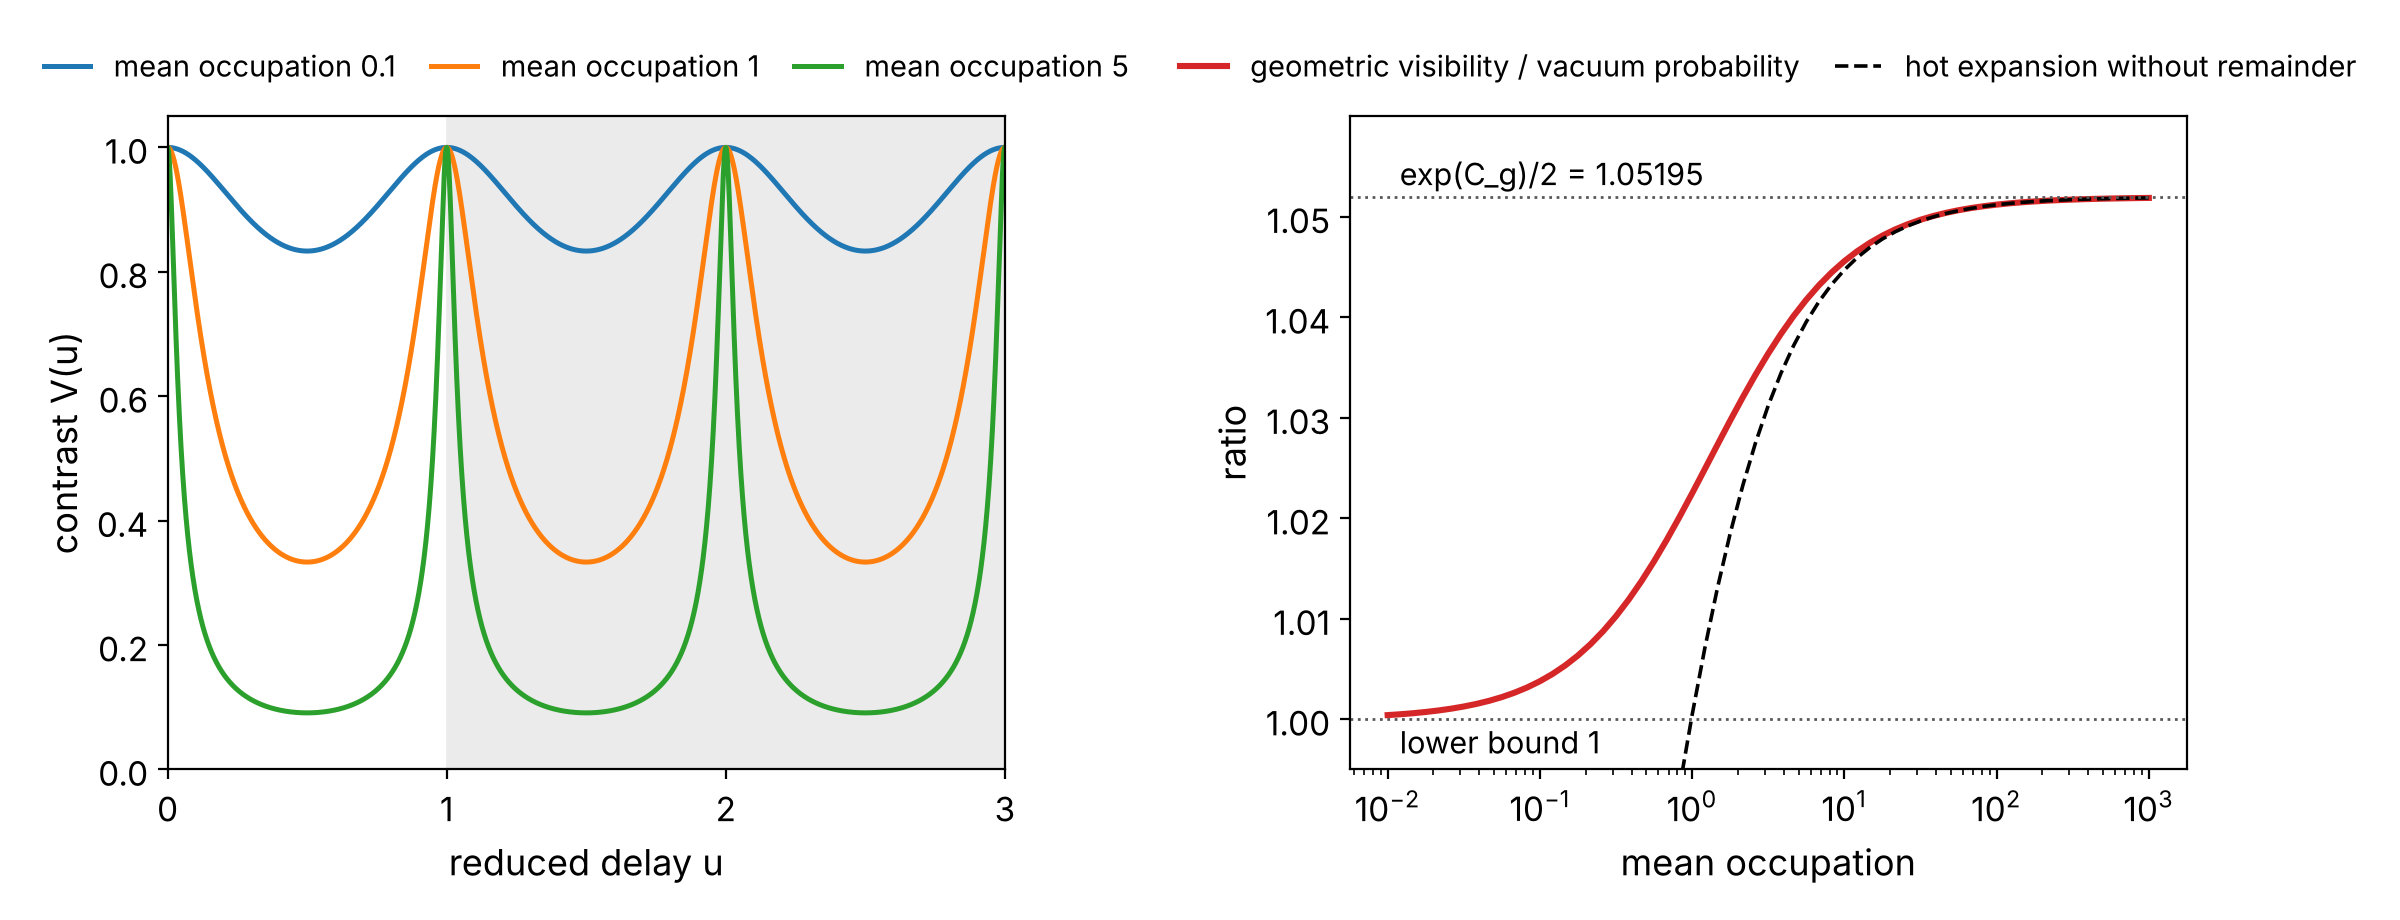
\includegraphics[width=\textwidth]{fig_bound.png}
\caption{Left: the contrast $V(u)$ of \CGeqref{eq:V} for $\bar n=0.1$, $1$ and $5$; the shaded region $u\ge1$ is the range of the geometric contrast \CGeqref{eq:Vs}. Right: the ratio $\mathcal V_1/p_0$ as a function of $\bar n$, between its sharp bounds $1$ and $\exp(C_g)/2$ of \CGeqref{eq:boundCg}, and the expansion \CGeqref{eq:hot} without its remainder.}\label{fig:bound}
\end{figure}

\begin{figure}[!htb]
\centering
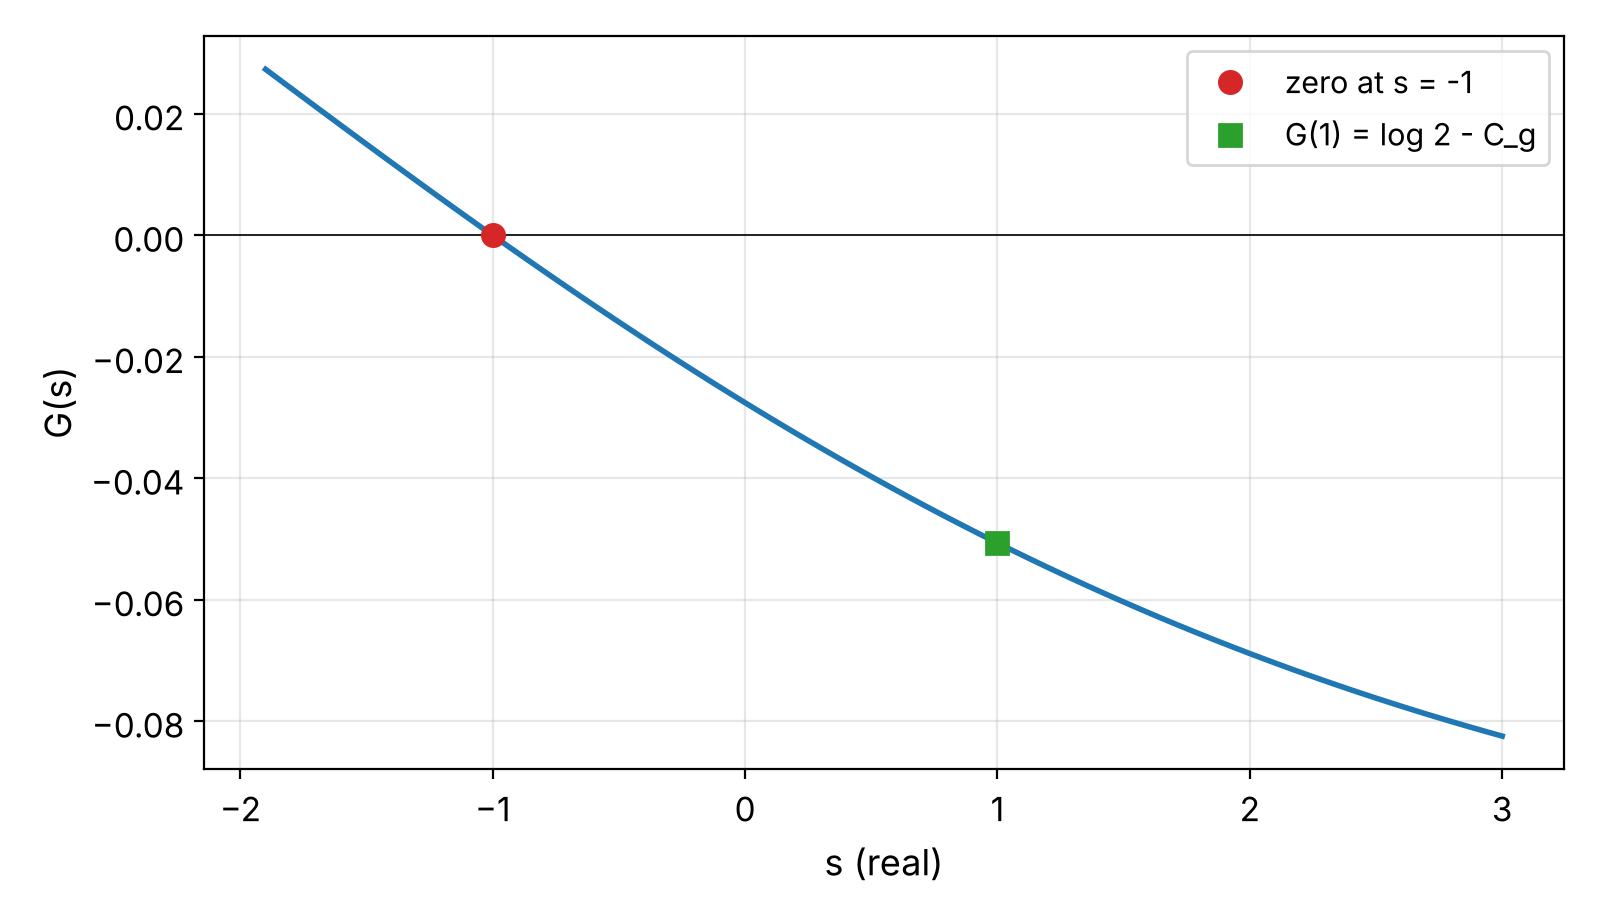
\includegraphics[width=.78\textwidth]{fig_G_real.png}
\caption{The function $G$ on the real axis. For $s>0$ the sharp constant of \CGeqref{eq:bound} is $e^{-sG(s)}$; the square marks $G(1)=\log2-C_g$.}\label{fig:Greal}
\end{figure}

At high temperature the ratio approaches its upper bound, and the approach can be made explicit.

\begin{theorem}\label{thm:hot}
Let $\bar n>0$ and $\tau=\log(1/q)=\log(1+1/\bar n)$. Then
\begin{equation}\label{eq:hot}
\log\mathcal V_1=\log p_0+C_g-\log2-\Big(\frac{\pi^2}{12}-\frac34\Big)\tau+R(\tau),\qquad R(\tau)>0,
\end{equation}
that is, $\mathcal V_1=\frac12\exp(C_g)\,p_0\,q^{\pi^2/12-3/4}\,e^{R(\tau)}$. For $0<\tau\le1$, that is, for $\bar n\ge1/(e-1)$,
\begin{equation}\label{eq:Rbound}
R(\tau)\le\frac{\tau^2}{\pi^2}\Big(\frac52+\frac12\log\frac1\tau\Big).
\end{equation}
\end{theorem}

\begin{proof}
Write $c_m=c_m(1)$ and $q^m=e^{-m\tau}$. By \CGeqref{eq:exact}, \CGeqref{eq:Cgseries} and \CGeqref{eq:sumcm},
\begin{equation}\label{eq:Rseries}
R(\tau)=\sum_{m\ge1}\frac{q^m}mc_m-\sum_{m\ge1}\frac{c_m}m+\tau\sum_{m\ge1}c_m=\sum_{m\ge1}\frac{c_m}m\big(m\tau-1+e^{-m\tau}\big) .
\end{equation}
For real $y>0$, $0<y-1+e^{-y}\le\min(y,\frac12y^2)$. Since $c_m>0$, this gives $R(\tau)>0$. With $c_m<1/(\pi^2m^2)$ from \CGeqref{eq:cmpos} it also gives
\begin{equation}\label{eq:Rmin}
R(\tau)\le\frac1{\pi^2}\sum_{m\ge1}\min\Big(\frac\tau{m^2},\frac{\tau^2}{2m}\Big).
\end{equation}
Let $0<\tau\le1$ and let $M=\lfloor1/\tau\rfloor\ge1$. Then $\sum_{m\le M}\frac1m\le1+\log M\le1+\log\frac1\tau$ and $\sum_{m>M}\frac1{m^2}<\frac1M\le2\tau$, because $\lfloor y\rfloor\ge\frac y2$ for $y\ge1$. Using the second entry of the minimum for $m\le M$ and the first for $m>M$, the sum in \CGeqref{eq:Rmin} is at most $\frac{\tau^2}2(1+\log\frac1\tau)+2\tau^2$.
\end{proof}

Table~\CGref{tab:values} gives the exact value of $\mathcal V_1$ from \CGeqref{eq:exact}, the ratio $\mathcal V_1/p_0$, the remainder $R(\tau)$ and its bound \CGeqref{eq:Rbound}. The bound \CGeqref{eq:Rbound} is not sharp: in the table the remainder is smaller than the bound by a factor between $2.9$ and $6$.

\begin{table}[!htb]
\caption{The geometric contrast $\mathcal V_1$ computed from \CGeqref{eq:exact}, its ratio to the vacuum probability $p_0$, the remainder $R(\tau)$ of \CGeqref{eq:hot} and the bound \CGeqref{eq:Rbound}, which applies when $\tau\le1$.}\label{tab:values}
\small
\begin{tabular}{rlllll}
\toprule
$\bar n$ & $p_0$ & $\mathcal V_1$ & $\mathcal V_1/p_0$ & $R(\tau)$ & bound \CGeqref{eq:Rbound}\\
\midrule
$0.01$ & $0.9900990$ & $0.9905007$ & $1.0004057$ & $2.84\times10^{-1}$ & \\
$0.1$ & $0.9090909$ & $0.9125237$ & $1.0037761$ & $1.27\times10^{-1}$ & \\
$1$ & $0.5000000$ & $0.5112376$ & $1.0224752$ & $2.18\times10^{-2}$ & $1.31\times10^{-1}$\\
$5$ & $0.1666667$ & $0.1734625$ & $1.0407747$ & $2.53\times10^{-3}$ & $1.13\times10^{-2}$\\
$20$ & $0.0476190$ & $0.0499291$ & $1.0485104$ & $2.58\times10^{-4}$ & $9.67\times10^{-4}$\\
$100$ & $0.0099010$ & $0.0104080$ & $1.0512094$ & $1.47\times10^{-5}$ & $4.82\times10^{-5}$\\
$1000$ & $0.0009990$ & $0.0010508$ & $1.0518762$ & $2.07\times10^{-7}$ & $6.03\times10^{-7}$\\
\bottomrule
\end{tabular}
\end{table}

A measured sequence of contrasts covers a finite range of delays. For real $U>1$ and $s>0$ let
\begin{equation}\label{eq:VsU}
\mathcal V_{s,U}=\exp\Big(\frac{s}{1-U^{-s}}\int_1^U\log V(u)\,u^{-s-1}\,du\Big),
\end{equation}
the geometric mean of the contrast over $1\le u\le U$ with the normalised weight.

\begin{proposition}\label{prop:trunc}
Let $\bar n>0$, $L=\log(2\bar n+1)$, $s>0$ and $U>1$. Then
\begin{equation}\label{eq:trunc}
\big|\log\mathcal V_{s,U}-\log\mathcal V_s\big|\le L\,U^{-s} .
\end{equation}
\end{proposition}

\begin{proof}
Put $X_1=s\int_1^U\log V(u)\,u^{-s-1}du$ and $X_2=s\int_U^\infty\log V(u)\,u^{-s-1}du$, so that $\log\mathcal V_s=X_1+X_2$ and $\log\mathcal V_{s,U}=X_1/(1-U^{-s})$. By Proposition~\CGref{prop:contrast}, $-L\le\log V(u)\le0$. Since $s\int_1^Uu^{-s-1}du=1-U^{-s}$ and $s\int_U^\infty u^{-s-1}du=U^{-s}$, we have $-L(1-U^{-s})\le X_1\le0$ and $-L\,U^{-s}\le X_2\le0$. The difference $\log\mathcal V_{s,U}-\log\mathcal V_s=X_1U^{-s}/(1-U^{-s})-X_2$ is thus the sum of a number in $[-L\,U^{-s},0]$ and a number in $[0,L\,U^{-s}]$.
\end{proof}

The bound \CGeqref{eq:trunc} uses only the range of $\log V$ and is not sharp: for $\bar n=20$, $s=1$ and $U=20$ it gives $0.186$, while the computed difference is $0.0025$.

\section{Damping, intrinsic dephasing and a nonlinear shift}\label{sec:real}

The returns of the contrast to $1$ rest on three idealisations: no damping of the mode, no intrinsic dephasing of the probe, and a shift exactly linear in the photon number. We bound the effect of the first and discuss the other two.

Let the mode be damped at the rate $\kappa>0$ by a bath with the same occupation $\bar n$, so that the thermal state of the mode is stationary. In the Lindblad description used for this problem \cite{Rigetti2012,ClerkUtami2007,Sears2012}, the state $\hat\rho$ of probe and mode obeys
\begin{equation}\label{eq:master}
\frac{d\hat\rho}{dt}=-i\big[\hat H,\hat\rho\big]+\kappa(\bar n+1)\,\mathcal L_{\hat a}\hat\rho+\kappa\bar n\,\mathcal L_{\hat a^\dagger}\hat\rho,\qquad \mathcal L_{\hat O}\hat\rho=\hat O\hat\rho\hat O^\dagger-\frac12\big(\hat O^\dagger\hat O\hat\rho+\hat\rho\hat O^\dagger\hat O\big),
\end{equation}
with $\hat H$ as in \CGeqref{eq:H}. Initially the probe is in $(\ket\uparrow+\ket\downarrow)/\sqrt2$, where $\hat\sigma_z\ket\uparrow=\ket\uparrow$ and $\hat\sigma_z\ket\downarrow=-\ket\downarrow$, and the mode is thermal. For $n\ge0$ let $\eta_n(t)$ be $2e^{i\omega_pt}$ times the diagonal element in the state with $n$ photons of the operator $\bra\uparrow\hat\rho(t)\ket\downarrow$ on the mode, so that $\eta_n(0)=p_n$. The coherence of the damped mode is $D_\kappa(t)=\sum_n\eta_n(t)$ and its contrast is $V_\kappa(t)=|D_\kappa(t)|$; without damping $D_\kappa(t)=D(\chi t/\pi)$. The operator $\bra\uparrow\hat\rho\ket\downarrow$ starts diagonal in the photon number, and the Hamiltonian part and both dissipators of \CGeqref{eq:master} map such operators to operators of the same kind. With $\eta_{-1}=0$ and
\begin{equation}\label{eq:rate}
\frac{d\eta_n}{dt}=-(2i\chi n+\Gamma_n)\,\eta_n+\kappa(\bar n+1)(n+1)\,\eta_{n+1}+\kappa\bar n\,n\,\eta_{n-1},\qquad \Gamma_n=\kappa\big[(\bar n+1)n+\bar n(n+1)\big],
\end{equation}
these are the rate equations of \cite{Sears2012} with the phase of each photon number added, the system solved in closed form in \cite{DykmanKrivoglaz1987,ClerkUtami2007}. The thermal distribution satisfies detailed balance: since $p_{n+1}=qp_n$ and $q(\bar n+1)=\bar n$,
\begin{equation}\label{eq:balance}
\kappa(\bar n+1)(n+1)\,p_{n+1}+\kappa\bar n\,n\,p_{n-1}=\Gamma_n\,p_n,\qquad n\ge0 .
\end{equation}

\begin{proposition}\label{prop:damp}
Let $(\eta_n)$ be the solution of \CGeqref{eq:rate} with $\eta_n(0)=p_n$ for which $\sum_n(n+1)|\eta_n(t)|$ is bounded on bounded intervals of $t$; this is the solution given by the density operator, whose mean energy is finite. Then, for every $t\ge0$,
\begin{equation}\label{eq:damp}
\big|D_\kappa(t)-D(\chi t/\pi)\big|\le2\sum_{n\ge0}p_n\big(1-e^{-\Gamma_nt}\big)\le\Lambda\,\kappa\,t,\qquad\Lambda=4\bar n(\bar n+1),
\end{equation}
and in particular $|V_\kappa(t)-V(u)|\le\pi\Lambda\,(\kappa/\chi)\,u$ with $u=\chi t/\pi$.
\end{proposition}

\begin{proof}
Step 1: $|\eta_n(t)|\le p_n$ for all $n$ and $t\ge0$. Let $\psi_n=|\eta_n|$ and $\Delta_n=\max(\psi_n-p_n,0)$. Since $\operatorname{Re}\big(\bar\eta_n\cdot(-2i\chi n)\eta_n\big)=0$, \CGeqref{eq:rate} gives, for $t_1<t_2$,
\begin{equation}\label{eq:psiineq}
\psi_n(t_2)-\psi_n(t_1)\le\int_{t_1}^{t_2}\Big(-\Gamma_n\psi_n+\kappa(\bar n+1)(n+1)\psi_{n+1}+\kappa\bar n\,n\,\psi_{n-1}\Big)dr .
\end{equation}
Subtracting \CGeqref{eq:balance} and using $\psi_k-p_k\le\Delta_k$, the same inequality holds for $\Delta_n$ on every interval on which $\psi_n>p_n$, with $\Delta$ in place of $\psi$. Since $\Delta_n$ is absolutely continuous, vanishes at $t=0$ and is constant on the intervals where it is $0$, this gives $\Delta_n(t)\le\int_0^t\big(-\Gamma_n\Delta_n+\kappa(\bar n+1)(n+1)\Delta_{n+1}+\kappa\bar n\,n\,\Delta_{n-1}\big)dr$. Sum over $n$. The sums converge, because $\Gamma_n\le\kappa(2\bar n+1)(n+1)$ and $\sum_n(n+1)(\psi_n+p_n)$ is bounded on $[0,t]$, and the gain terms add up to $\sum_k\big(\kappa(\bar n+1)k+\kappa\bar n(k+1)\big)\Delta_k=\sum_k\Gamma_k\Delta_k$. So $\sum_n\Delta_n(t)\le0$, and every $\Delta_n(t)$ is $0$.

Step 2. Put $F_n(r)=\kappa(\bar n+1)(n+1)\eta_{n+1}(r)+\kappa\bar n\,n\,\eta_{n-1}(r)$. Solving \CGeqref{eq:rate} as a linear equation for $\eta_n$,
\begin{equation}\label{eq:duhamel}
\eta_n(t)=p_n\,e^{-(2i\chi n+\Gamma_n)t}+\int_0^te^{-(2i\chi n+\Gamma_n)(t-r)}\,F_n(r)\,dr .
\end{equation}
By Step 1 and \CGeqref{eq:balance}, $|F_n(r)|\le\Gamma_np_n$. Hence
\begin{equation}\label{eq:etadiff}
\big|\eta_n(t)-p_n\,e^{-2i\chi nt}\big|\le p_n\big(1-e^{-\Gamma_nt}\big)+\int_0^te^{-\Gamma_n(t-r)}\,\Gamma_np_n\,dr=2p_n\big(1-e^{-\Gamma_nt}\big).
\end{equation}
Summing over $n$, with $D(\chi t/\pi)=\sum_np_ne^{-2i\chi nt}$, gives the first inequality of \CGeqref{eq:damp}. Since $1-e^{-y}\le y$ for $y\ge0$ and $\sum_nnp_n=\bar n$, the sum is at most $2t\sum_np_n\Gamma_n=2\kappa t\big((\bar n+1)\bar n+\bar n(\bar n+1)\big)=\Lambda\kappa t$. Finally $\big||a|-|b|\big|\le|a-b|$ and $t=\pi u/\chi$.
\end{proof}

For the geometric contrast of the damped mode over $1\le u\le U$, $\mathcal V^\kappa_{s,U}$, defined by \CGeqref{eq:VsU} with $V_\kappa(\pi u/\chi)$ in place of $V(u)$, the bound gives the following.

\begin{corollary}\label{cor:damp}
Let $s>0$, $U>1$, and suppose that $\epsilon=\pi\Lambda(2\bar n+1)(\kappa/\chi)\,U<1$. Then
\begin{equation}\label{eq:dampfun}
\big|\log\mathcal V^\kappa_{s,U}-\log\mathcal V_{s,U}\big|\le-\log(1-\epsilon),\qquad\Big|\log V_\kappa\Big(\frac\pi{2\chi}\Big)-\log V\Big(\frac12\Big)\Big|\le-\log\Big(1-\frac\epsilon{2U}\Big).
\end{equation}
\end{corollary}

\begin{proof}
For $0\le u\le U$, Proposition~\CGref{prop:damp} and $V(u)\ge1/(2\bar n+1)$ give $|V_\kappa(\pi u/\chi)-V(u)|\le\pi\Lambda(\kappa/\chi)U=\epsilon/(2\bar n+1)\le\epsilon V(u)$. So $1-\epsilon\le V_\kappa/V\le1+\epsilon$ and $|\log(V_\kappa/V)|\le-\log(1-\epsilon)$, because $\log(1+\epsilon)\le-\log(1-\epsilon)$. The weight in \CGeqref{eq:VsU} is a probability measure on $[1,U]$. At $u=\frac12$, Proposition~\CGref{prop:damp} gives $|V_\kappa(\frac\pi{2\chi})-V(\frac12)|\le\pi\Lambda(\kappa/\chi)/2=\epsilon/(2U(2\bar n+1))\le\frac\epsilon{2U}V(\frac12)$, and the logarithm is bounded as before with $\frac\epsilon{2U}$ in place of $\epsilon$.
\end{proof}

The condition $\epsilon<1$ asks for $\kappa/\chi<1/\big(\pi\Lambda(2\bar n+1)U\big)$, which decreases as $\bar n^{-3}$. With $U=20$ and $\epsilon=0.1$ it reads $\kappa/\chi<3.0\times10^{-3}$ for $\bar n=0.1$, $\kappa/\chi<6.6\times10^{-5}$ for $\bar n=1$ and $\kappa/\chi<2.3\times10^{-8}$ for $\bar n=20$. For $\chi/2\pi=1$~MHz these are $\kappa/2\pi<3.0$~kHz, $66$~Hz and $0.023$~Hz. Cavity linewidths $\kappa/2\pi$ between $6$ and $120$~kHz are reported in \cite{Sears2012}, and a single-photon lifetime of $25.6$~ms, that is $\kappa/2\pi=6.2$~Hz, in \cite{Milul2023}. The geometric contrast is therefore usable at low occupation in long-lived modes, and the statements of Section~\CGref{sec:main} at high occupation, such as the example $\bar n=20$ after Corollary~\CGref{cor:bracket}, are statements about the ideal model only. The half-period contrast is affected less, by the factor $1/(2U)$ in \CGeqref{eq:dampfun}, because its delay is short. The bound \CGeqref{eq:damp} is not sharp: for $\bar n$ in $\{0.05,1,5,20\}$, $\kappa/(2\chi)$ between $10^{-5}$ and $10^{-2}$ and $0<u\le6$, the difference $|V_\kappa-V|$ computed from the closed form of \cite{ClerkUtami2007} is at most $0.51$ times the bound.

Intrinsic dephasing of the probe. If, independently of the photons, the probe has a coherence factor $f(t)$ with $0<f(t)\le1$, the measured contrast without damping is $f(t)V(u)$. Since $V(k)=1$ at the returns, the contrast measured at $u=k$ is $f(\pi k/\chi)$: the returns measure the decay of the probe itself, which can then be divided out. Without that correction, a factor $f(t)=e^{-t/T}$ changes $\log\mathcal V_{1,U}$ by
\begin{equation}\label{eq:Tdeph}
\frac1{1-U^{-1}}\int_1^U\Big(-\frac{\pi u}{\chi T}\Big)u^{-2}\,du=-\frac{\pi}{\chi T}\cdot\frac{U\log U}{U-1} .
\end{equation}

Nonlinear shift. If the phase acquired by the component with $n$ photons is not exactly $2\chi nt$, for example $2\chi nt+\chi_2n(n-1)t$ with a real $\chi_2\ne0$, the contrast at the return $u=k$ becomes $\big|\sum_np_ne^{-i\pi k\chi_2n(n-1)/\chi}\big|$, which is below $1$ in general. With the decay of the probe divided out, a measured contrast below $1$ at the returns therefore signals damping or a nonlinear shift, and Proposition~\CGref{prop:damp} bounds the part due to damping. None of the results of Sections~\CGref{sec:main}, \CGref{sec:sum} and~\CGref{sec:GA} is claimed for a nonlinear shift.

\section{The sum rule and the harmonic delays}\label{sec:sum}

The first return divides the delays into the interval $0<u<1$ and the half-line $u\ge1$. Over all delays together the integral of the logarithm of the contrast is linear in the occupation.

\begin{proposition}\label{prop:sum}
For every $\bar n>0$,
\begin{equation}\label{eq:sumrule}
\int_0^\infty\log V(u)\,u^{-2}\,du=-\pi^2\,\bar n,\qquad \int_0^1\log V(u)\,u^{-2}\,du=-\pi^2\,\bar n-\log\mathcal V_1 .
\end{equation}
\end{proposition}

\begin{proof}
By \CGeqref{eq:logV} and $\log(1-q)=-\sum_mq^m/m$, $\log V(u)=\sum_{m\ge1}\frac{q^m}m\big(\cos(2\pi mu)-1\big)$, a series of terms that are all $\le0$, so by Tonelli's theorem it may be integrated term by term. Let $\lambda>0$ and $0<\delta<Y$. Integration by parts gives $\int_\delta^Y(1-\cos\lambda u)u^{-2}du=\frac{1-\cos\lambda\delta}{\delta}-\frac{1-\cos\lambda Y}{Y}+\lambda\int_\delta^Y\frac{\sin\lambda u}u\,du$. As $\delta\to0$ and $Y\to\infty$ the first two terms tend to $0$ and the last integral tends to $\frac\pi2$, by the classical Dirichlet integral \cite[(6.2.9), (6.2.14)]{DLMF}. Hence $\int_0^\infty(1-\cos\lambda u)u^{-2}du=\frac{\pi\lambda}2$. With $\lambda=2\pi m$,
\begin{equation}\label{eq:sumproof}
\int_0^\infty\log V(u)\,u^{-2}\,du=-\sum_{m\ge1}\frac{q^m}m\,\pi^2m=-\pi^2\,\frac q{1-q}=-\pi^2\,\bar n .
\end{equation}
The second identity of \CGeqref{eq:sumrule} follows from $\int_1^\infty\log V(u)u^{-2}du=\log\mathcal V_1$, which is \CGeqref{eq:Vs} with $s=1$.
\end{proof}

By \CGeqref{eq:boundCg} the part of the sum rule that lies after the first return, $\log\mathcal V_1$, differs from $\log p_0$ by less than $C_g-\log2=0.0506\ldots$ for every positive occupation. The part before the first return carries the linear term $-\pi^2\bar n$.

The logarithm of the geometric contrast is also the logarithmic rate of decay of a product. For an integer $N\ge2$ let
\begin{equation}\label{eq:PN}
\mathcal P(N)=\prod_{k=1}^{N-1}V\Big(\frac Nk\Big).
\end{equation}
This is the product of the contrasts measured at the harmonic delays $u_k=N/k$, that is, at the times $N\pi/(k\chi)$. It is also the contrast at the time $N\pi/\chi$ of a probe coupled to $N-1$ independent modes with dispersive couplings $\chi/k$, $1\le k\le N-1$, and equal occupation $\bar n$, because the coherences of independent modes multiply.

\begin{proposition}\label{prop:harm}
Let $\bar n>0$, $L=\log(2\bar n+1)$ and let $N\ge2$ be an integer. Then
\begin{equation}\label{eq:harm}
\Big|\frac1N\log\mathcal P(N)-\log\mathcal V_1\Big|\le L\,\Big(\frac{2\sqrt2}{\sqrt N}+\frac1N\Big).
\end{equation}
In particular $\mathcal P(N)^{1/N}\to\mathcal V_1$ as $N\to\infty$, and by \CGeqref{eq:boundCg} this limit lies strictly between $p_0$ and $\frac12\exp(C_g)p_0$.
\end{proposition}

\begin{proof}
By Proposition~\CGref{prop:contrast} the function $\log V$ has period $1$ and takes values in $[-L,0]$. On each interval $[j,j+\frac12]$ with integer $j$ it decreases from $0$ to $-L$, and on $[j+\frac12,j+1]$ it increases from $-L$ to $0$. Put $u_k=N/k$ for $1\le k\le N$, so that $u_N=1$ and $u_1=N$, and $I_k=[u_{k+1},u_k]$ for $1\le k\le N-1$. The intervals $I_k$ cover $[1,N]$ and overlap only at end points, and $\int_{I_k}u^{-2}du=\frac{k+1}N-\frac kN=\frac1N$. Therefore
\begin{equation}\label{eq:riemann}
\frac1N\log\mathcal P(N)-\int_1^N\log V(u)\,u^{-2}\,du=\sum_{k=1}^{N-1}\int_{I_k}\big(\log V(u_k)-\log V(u)\big)\,u^{-2}\,du .
\end{equation}
The $k$-th term has modulus at most $\frac1N$ times the oscillation of $\log V$ on $I_k$, which is at most $L$ and at most the total variation of $\log V$ on $I_k$. Let $k_0$ be an integer with $1\le k_0\le N-1$. The intervals $I_k$ with $k>k_0$ cover $[1,u_{k_0+1}]$ and overlap only at end points, so the sum of the total variations on them is the total variation on $[1,u_{k_0+1}]$. An interval $[1,x]$ with $x\ge1$ is covered by the intervals of monotonicity $[\frac j2,\frac{j+1}2]$ with $2\le j\le\lceil2x\rceil-1$, at most $2x-1$ in number, on each of which the variation is at most $L$. So the total variation of $\log V$ on $[1,x]$ is at most $2Lx$. The right side of \CGeqref{eq:riemann} is thus at most $\frac LN\big(k_0+\frac{2N}{k_0+1}\big)$ in modulus. Choose $k_0=\lceil\sqrt{2N}\rceil-1$. Since $N\ge2$, $2\le\sqrt{2N}\le N$, so $1\le k_0\le N-1$, and $k_0<\sqrt{2N}\le k_0+1$. Then $k_0+\frac{2N}{k_0+1}<2\sqrt{2N}$, which gives the first term of \CGeqref{eq:harm}. Finally $\big|\int_N^\infty\log V(u)u^{-2}du\big|\le\frac LN$, and $\int_1^\infty\log V(u)u^{-2}du=\log\mathcal V_1$.
\end{proof}

At zero temperature the factors of the same product, formed with $2|\sin(\pi N/k)|$ in place of the contrast, vanish whenever $k$ divides $N$. The thermal factors do not vanish: by Proposition~\CGref{prop:contrast} each of them is at least $1/(2\bar n+1)$, and a divisor $k$ of $N$ contributes the factor $1$.

\section{The transforms after and before the first return and their zeros}\label{sec:GA}

Theorem~\CGref{thm:main} uses $G$ on the positive real axis. At complex exponents the same function describes the hot limit of the contrast against weights that oscillate in the logarithm of the delay.

\begin{proposition}\label{prop:complex}
For $\sigma>0$,
\begin{equation}\label{eq:complexlimit}
\lim_{\bar n\to\infty}\int_1^\infty\log\frac{V(u)}{p_0}\,u^{-s-1}\,du=-G(s),
\end{equation}
uniformly for $s$ in compact subsets of the half-plane $\sigma>0$.
\end{proposition}

\begin{proof}
By \CGeqref{eq:logV} the integral is $-G_q(s)$. By \CGeqref{eq:Gseries}, $|G_q(s)-G(s)|\le\sum_{m\ge1}(1-q^m)|c_m(s)|/m$. By \CGeqref{eq:cmbound} the series $\sum_m|c_m(s)|/m$ converges uniformly on compact subsets of $\sigma>-2$, and each term of the bound tends to $0$ as $q\to1^-$, so the bound tends to $0$ uniformly there.
\end{proof}

For real $s>0$ the limit \CGeqref{eq:complexlimit} is positive and gives the sharp constants of Theorem~\CGref{thm:main}. For $s=\sigma+i\theta$ with $\theta\ne0$ the weight is $u^{-\sigma-1}e^{-i\theta\log u}$. At a zero of $G$ with $\sigma>0$ the limit vanishes: the excess $\log(V/p_0)$ of a hot mode has no component on that weight. Table~\CGref{tab:zeros} lists the zeros of $G$ computed in the rectangle $0<\sigma<2$, $0<\theta\le40$, and Figure~\CGref{fig:Gsurf} shows $|G|$ there.

\begin{figure}[!htb]
\centering
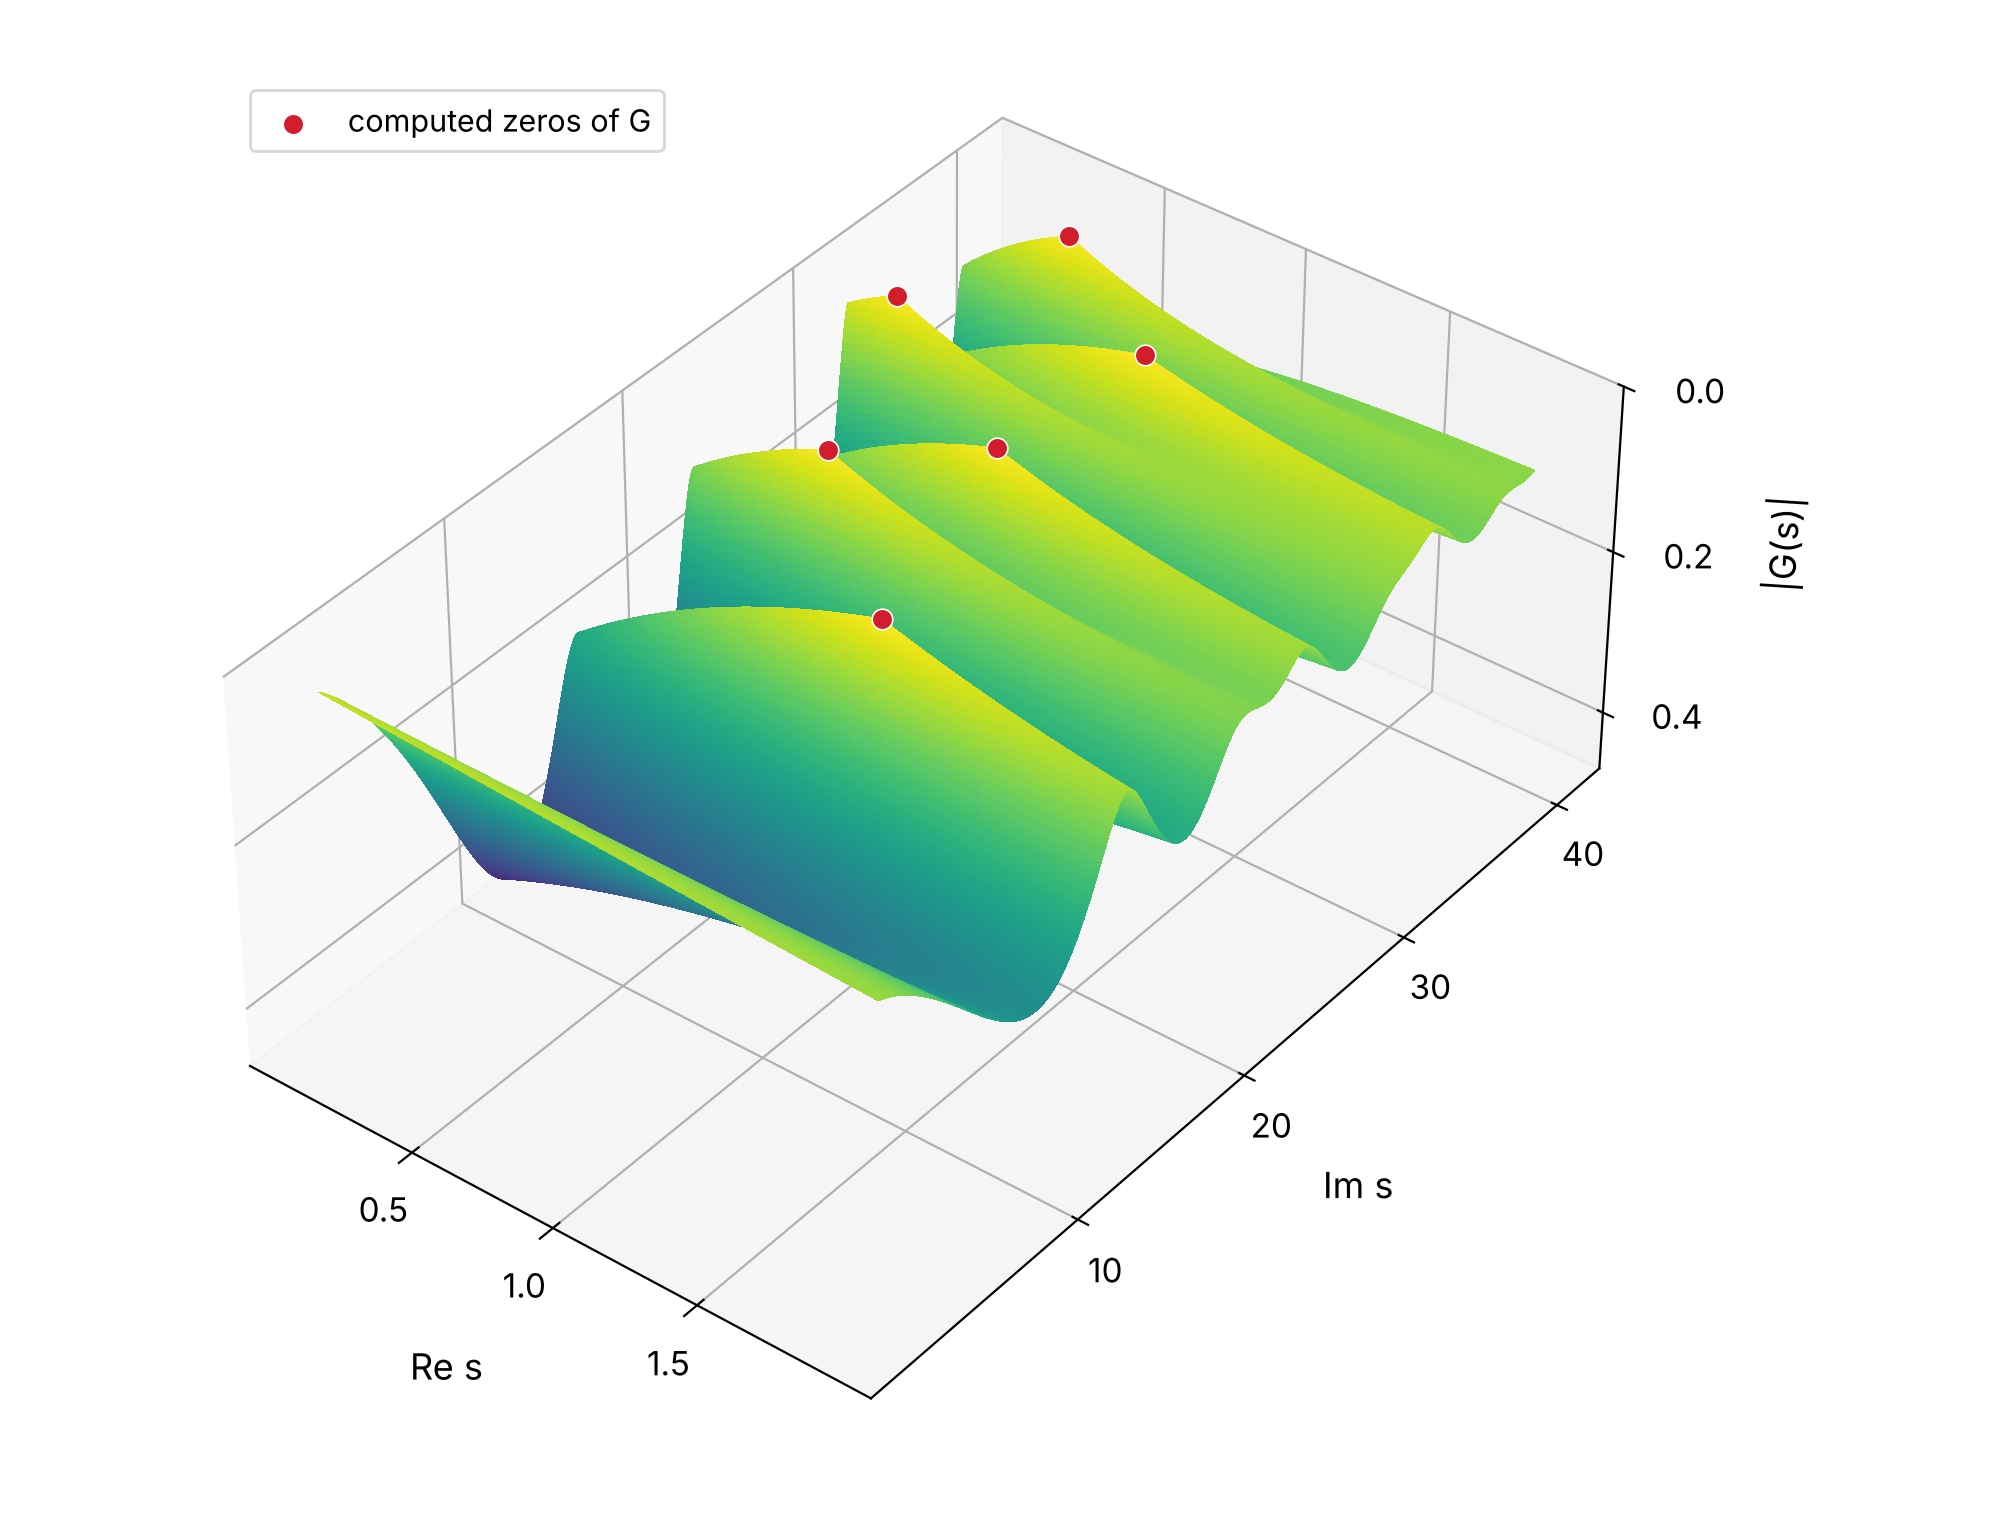
\includegraphics[width=.80\textwidth]{fig_G_surface.png}
\caption{$|G(s)|$ on the rectangle $0.05\le\operatorname{Re}s\le1.95$, $1\le\operatorname{Im}s\le40$, on a linear vertical axis that is inverted, so that a zero is a peak. The red markers are the six computed zeros of $G$ of Table~\CGref{tab:zeros}.}\label{fig:Gsurf}
\end{figure}

The delays before the first return enter through a second function. The weight $u^{-s-1}$ is not integrable at $u=0$ against $h$, which behaves there as $\log(2\pi u)$. Subtracting this short-time form gives, for $\sigma<2$ and $s\ne0$,
\begin{equation}\label{eq:A}
A(s)=\frac{\log(2\pi)}s+\frac1{s^2}-\int_0^1\log\frac{\sin(\pi u)}{\pi u}\,u^{-s-1}\,du .
\end{equation}
The integral converges absolutely for $\sigma<2$, because the logarithm is $O(u^2)$ as $u\to0$ and has an integrable singularity at $u=1$. Let $\zeta$ denote the Riemann zeta function, $\zeta(s)=\sum_{j\ge1}j^{-s}$ for $\sigma>1$, continued analytically to the complex plane with a simple pole at $s=1$.

\begin{proposition}\label{prop:A}
(a) For $\sigma<2$ and $s\ne0$,
\begin{equation}\label{eq:Aseries}
A(s)=\frac{\log(2\pi)}s+\frac1{s^2}+\sum_{k\ge1}\frac{\zeta(2k)}{k\,(2k-s)} .
\end{equation}
The series converges for every complex $s$ other than $2,4,6,\dots$ and continues $A$ to a meromorphic function on the complex plane.

(b) For $0<\sigma<2$,
\begin{equation}\label{eq:GAzeta}
G(s)-A(s)=\frac\pi s\cot\Big(\frac{\pi s}2\Big)\,\zeta(s),
\end{equation}
where the right side is continued analytically to $s=1$, with value $-\frac{\pi^2}2$.

(c) For non-real $s$ with $0<\sigma<2$, $G(s)=A(s)$ if and only if $\zeta(s)=0$.
\end{proposition}

\begin{proof}
(a) By the product for the sine \cite[(4.22.1)]{DLMF}, $\sin(\pi u)=\pi u\prod_{j\ge1}(1-u^2/j^2)$. For $0<u<1$ every factor lies in $(0,1)$ and
\begin{equation}\label{eq:logsinc}
\log\frac{\sin(\pi u)}{\pi u}=\sum_{j\ge1}\log\Big(1-\frac{u^2}{j^2}\Big)=-\sum_{j\ge1}\sum_{k\ge1}\frac{u^{2k}}{k\,j^{2k}}=-\sum_{k\ge1}\frac{\zeta(2k)}k\,u^{2k},
\end{equation}
a double series of terms of one sign. For $\sigma<2$, $\int_0^1u^{2k-s-1}du=\frac1{2k-s}$, and $\sum_k\frac{\zeta(2k)}{k(2k-\sigma)}<\infty$. Integrating \CGeqref{eq:logsinc} term by term in \CGeqref{eq:A} gives \CGeqref{eq:Aseries}. Since $\zeta(2k)\le\zeta(2)$, the terms are $O(k^{-2})$ uniformly on compact sets that avoid the points $2k$, which gives the continuation.

(b) For $\sigma>0$, $\int_1^\infty\log(2\pi u)\,u^{-s-1}du=\frac{\log(2\pi)}s+\frac1{s^2}$. For $0<u<1$, $h(u)-\log(2\pi u)=\log\frac{\sin(\pi u)}{\pi u}$. Hence, for $0<\sigma<2$,
\begin{equation}\label{eq:GAint}
G(s)-A(s)=\int_0^\infty\big(h(u)-\log(2\pi u)\big)\,u^{-s-1}\,du .
\end{equation}
By the product for the sine, $h(u)-\log(2\pi u)=\sum_{j\ge1}\log|1-u^2/j^2|$ for every $u>0$ that is not an integer. For $0<\sigma<2$ put
\begin{equation}\label{eq:Ksigma}
K_\sigma=\int_0^\infty\big|\log|1-v^2|\big|\,v^{-\sigma-1}\,dv<\infty .
\end{equation}
It is finite because the logarithm is $O(v^2)$ at $0$, has an integrable singularity at $1$ and is $O(\log v)$ at infinity. The substitution $u=jv$ gives $\int_0^\infty\big|\log|1-u^2/j^2|\big|u^{-\sigma-1}du=j^{-\sigma}K_\sigma$. Let $1<\sigma<2$. Then $\sum_jj^{-\sigma}K_\sigma<\infty$, the sum over $j$ may be exchanged with the integral in \CGeqref{eq:GAint}, and
\begin{equation}\label{eq:J}
G(s)-A(s)=\zeta(s)\,J(s),\qquad J(s)=\int_0^\infty\log|1-v^2|\,v^{-s-1}\,dv .
\end{equation}
We compute $J(s)$ for $0<\sigma<2$. On $(0,1)$, $\log(1-v^2)=-\sum_{k\ge1}v^{2k}/k$ with terms of one sign, so $\int_0^1\log(1-v^2)\,v^{-s-1}dv=-\sum_k\frac1{k(2k-s)}$. On $(1,\infty)$ substitute $v=1/w$: $\int_1^\infty\log(v^2-1)\,v^{-s-1}dv=\int_0^1\big(\log(1-w^2)-2\log w\big)w^{s-1}dw=-\sum_k\frac1{k(2k+s)}+\frac2{s^2}$. Adding the two parts,
\begin{equation}\label{eq:Jsum}
J(s)=\frac2{s^2}-\sum_{k\ge1}\frac1k\Big(\frac1{2k-s}+\frac1{2k+s}\Big)=\frac2{s^2}-\sum_{k\ge1}\frac1{k^2-s^2/4} .
\end{equation}
The partial fractions of the cotangent \cite[(4.22.3)]{DLMF}, at the point $\frac{\pi s}2$, which is not a multiple of $\pi$, read $\cot\frac{\pi s}2=\frac2{\pi s}-\frac s\pi\sum_{k\ge1}\frac1{k^2-s^2/4}$. Multiplying by $\frac\pi s$ and comparing with \CGeqref{eq:Jsum} gives $J(s)=\frac\pi s\cot\frac{\pi s}2$. This proves \CGeqref{eq:GAzeta} for $1<\sigma<2$. Both sides are analytic in the strip $0<\sigma<2$: $G$ by Lemma~\CGref{lem:G}, $A$ by \CGeqref{eq:A}, and the right side because the simple pole of $\zeta$ at $s=1$ is cancelled by the zero of the cotangent. So \CGeqref{eq:GAzeta} holds in the strip. Near $s=1$, $\cot\frac{\pi s}2=-\frac\pi2(s-1)+O((s-1)^3)$ and $\zeta(s)=\frac1{s-1}+O(1)$, which gives the value $-\frac{\pi^2}2$.

(c) For non-real $s$ the number $\frac{\pi s}2$ is not real, so $\cot\frac{\pi s}2$ is finite and different from $0$, and $\frac\pi s\ne0$. By \CGeqref{eq:GAzeta}, $G(s)-A(s)$ is the product of $\zeta(s)$ and a finite non-zero number, so each of $G(s)=A(s)$ and $\zeta(s)=0$ implies the other.
\end{proof}

By \CGeqref{eq:GAint} the difference $G-A$ is the transform over all delays of $h$ relative to its short-time form, and by \CGeqref{eq:GAzeta} it is the Riemann zeta function up to an elementary factor. The function $G$ carries the delays after the first return and $A$ the delays before it. By Proposition~\CGref{prop:A}(c) the two coincide at a non-real exponent of the strip exactly at the zeros of $\zeta$. This equivalence is a consequence of the explicit factor in \CGeqref{eq:GAzeta} and gives no information on the location of those zeros. Mellin representations of $\zeta$ over a half-line are classical; the simplest, $\zeta(s)=\frac s{s-1}-s\int_1^\infty(u-\lfloor u\rfloor)u^{-s-1}du$ for $\sigma>0$, follows for $\sigma>1$ from $\zeta(s)=s\int_1^\infty\lfloor u\rfloor u^{-s-1}du$ and extends to $\sigma>0$ because the integral is analytic there. The identity \CGeqref{eq:GAzeta} is of the same type.

Figures~\CGref{fig:Asurf} and~\CGref{fig:Areal} show $|A|$. On the grid of Figure~\CGref{fig:Asurf} the computed values of $|A|$ lie between $0.0721$ and $2.1831$, and no zero of $A$ is found there. Near the real axis the continuation \CGeqref{eq:Aseries} has the poles $0,2,4,\dots$ and real zeros, of which Table~\CGref{tab:zeros} lists those in $-3.5<s<9.5$. Figure~\CGref{fig:map} shows, in the rectangle of Figure~\CGref{fig:Gsurf}, the six computed zeros of $G$ and the six points with $G=A$. The latter are the points $\frac12+i\theta$ with $\theta=14.1347$, $21.0220$, $25.0109$, $30.4249$, $32.9351$, $37.5862$, the first six zeros of $\zeta$ in the upper half-plane.

\begin{table}[!htb]
\caption{Computed zeros of $G$ in the rectangle $0<\operatorname{Re}s<2$, $0<\operatorname{Im}s\le40$, and computed real zeros of the continuation \CGeqref{eq:Aseries} of $A$ in $-3.5<s<9.5$.}\label{tab:zeros}
\small
\begin{tabular}{ll}
\toprule
zeros of $G$ & real zeros of $A$\\
\midrule
$1.127313+15.001263\,i$ & $-2.0000$\\
$0.533572+21.763255\,i$ & $-1.0000$\\
$0.894731+25.624837\,i$ & $3.0428$\\
$0.227688+30.975963\,i$ & $5.0981$\\
$0.950507+33.599088\,i$ & $7.1478$\\
$0.430900+38.054886\,i$ & $9.1892$\\
\bottomrule
\end{tabular}
\end{table}

\begin{figure}[!p]
\centering
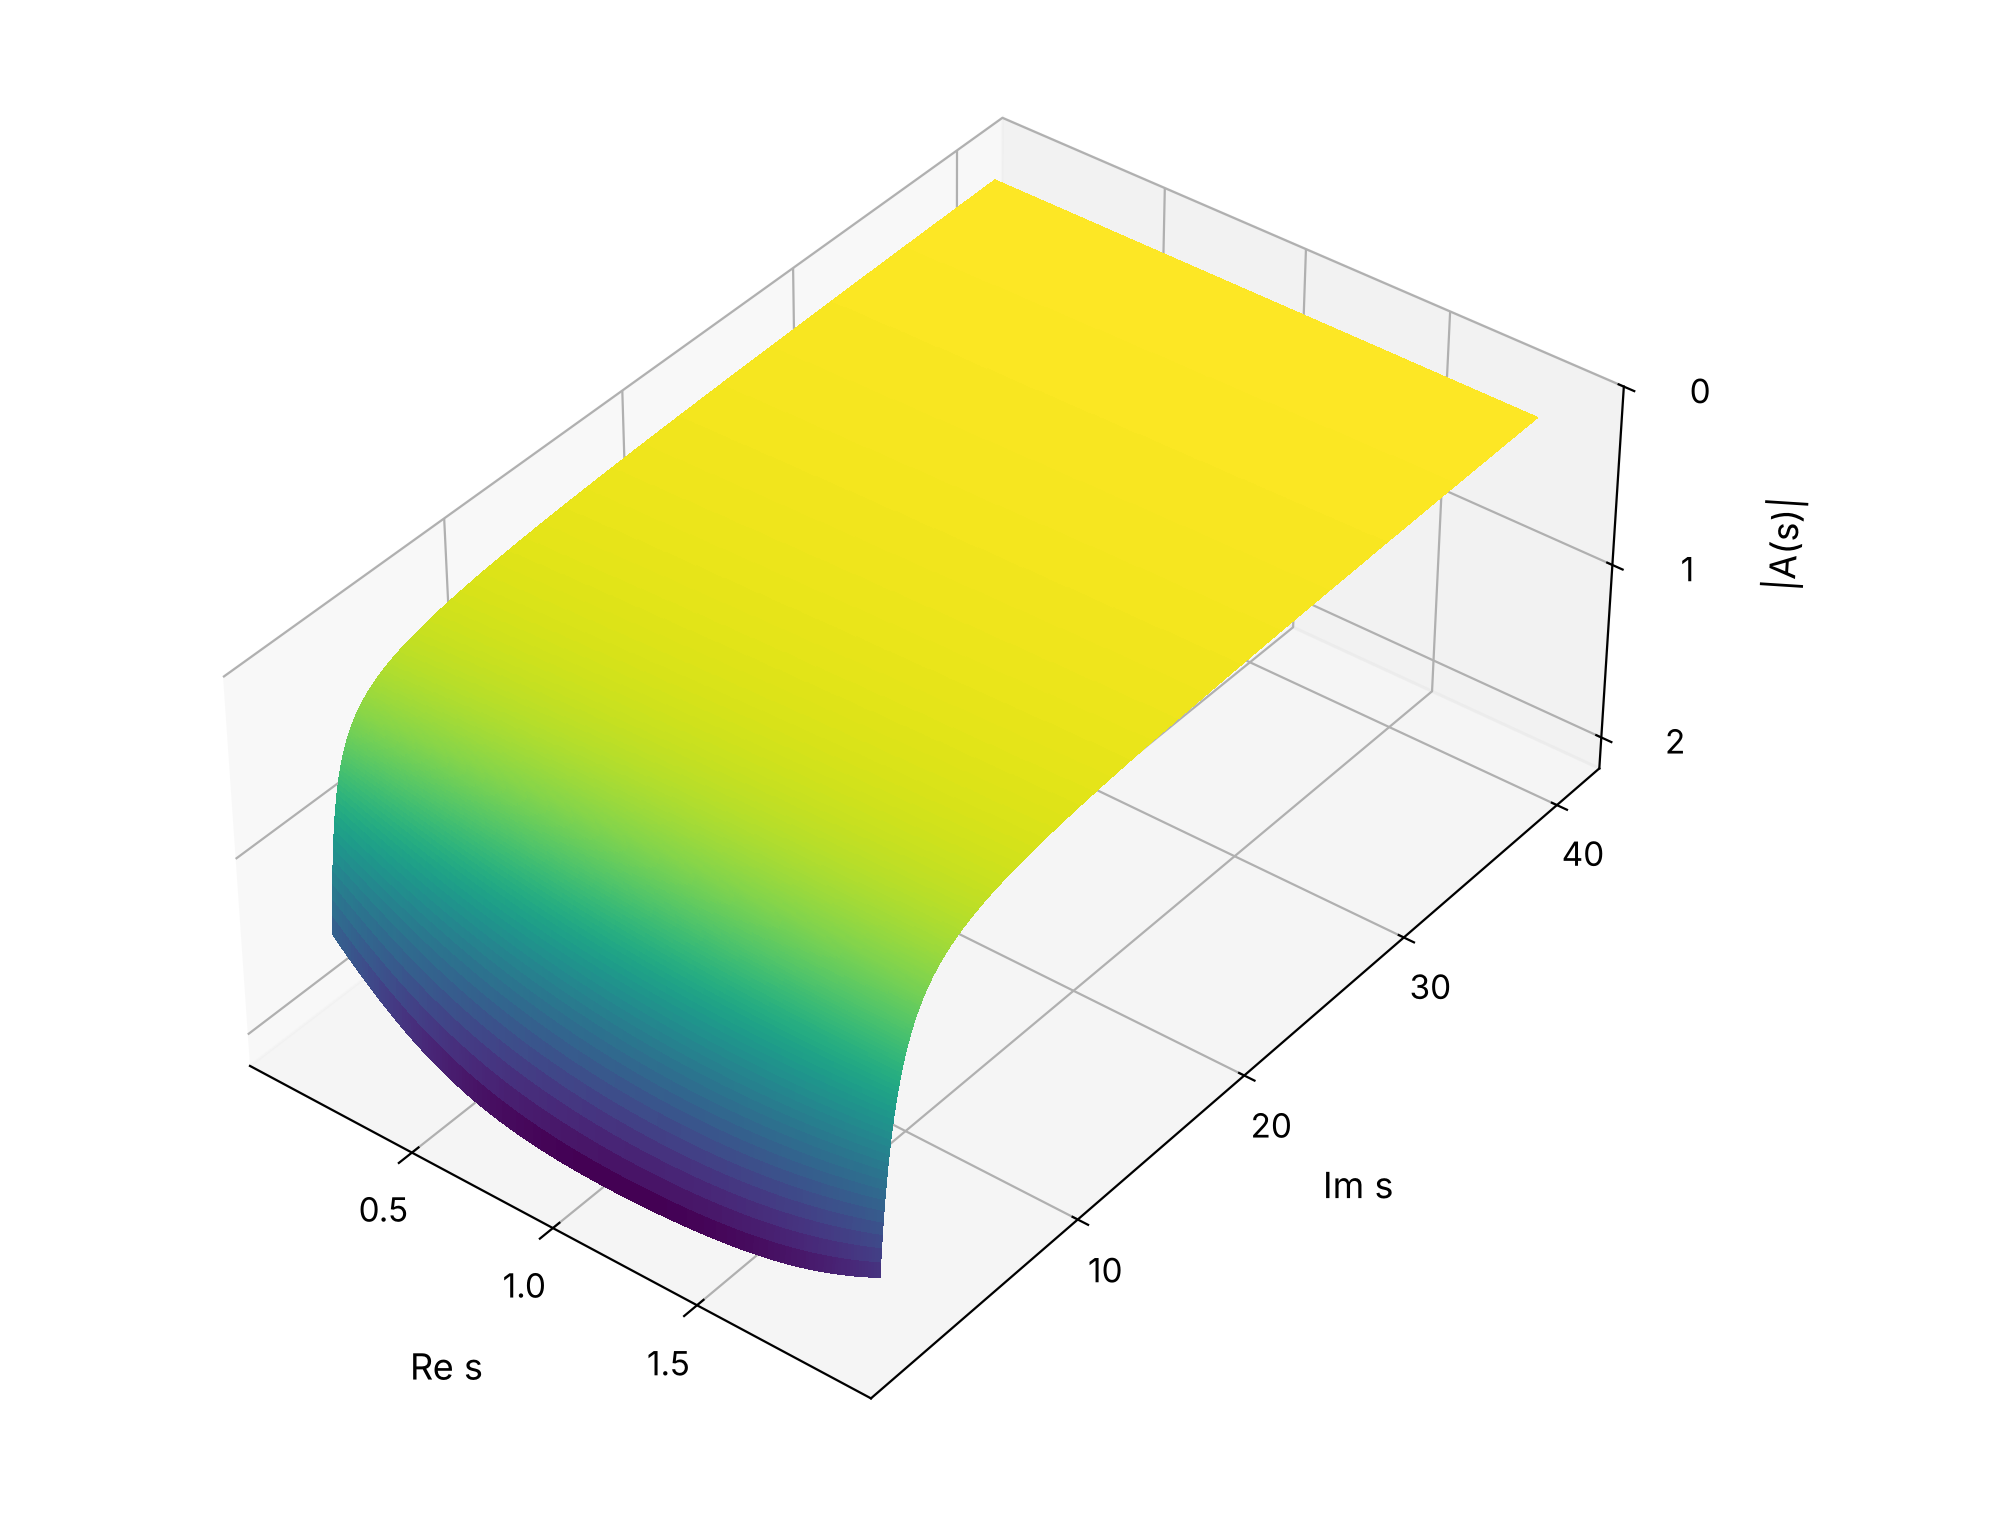
\includegraphics[width=.72\textwidth]{fig_A_surface.png}
\caption{$|A(s)|$ on the rectangle of Figure~\CGref{fig:Gsurf}, with the vertical axis inverted.}\label{fig:Asurf}

\bigskip
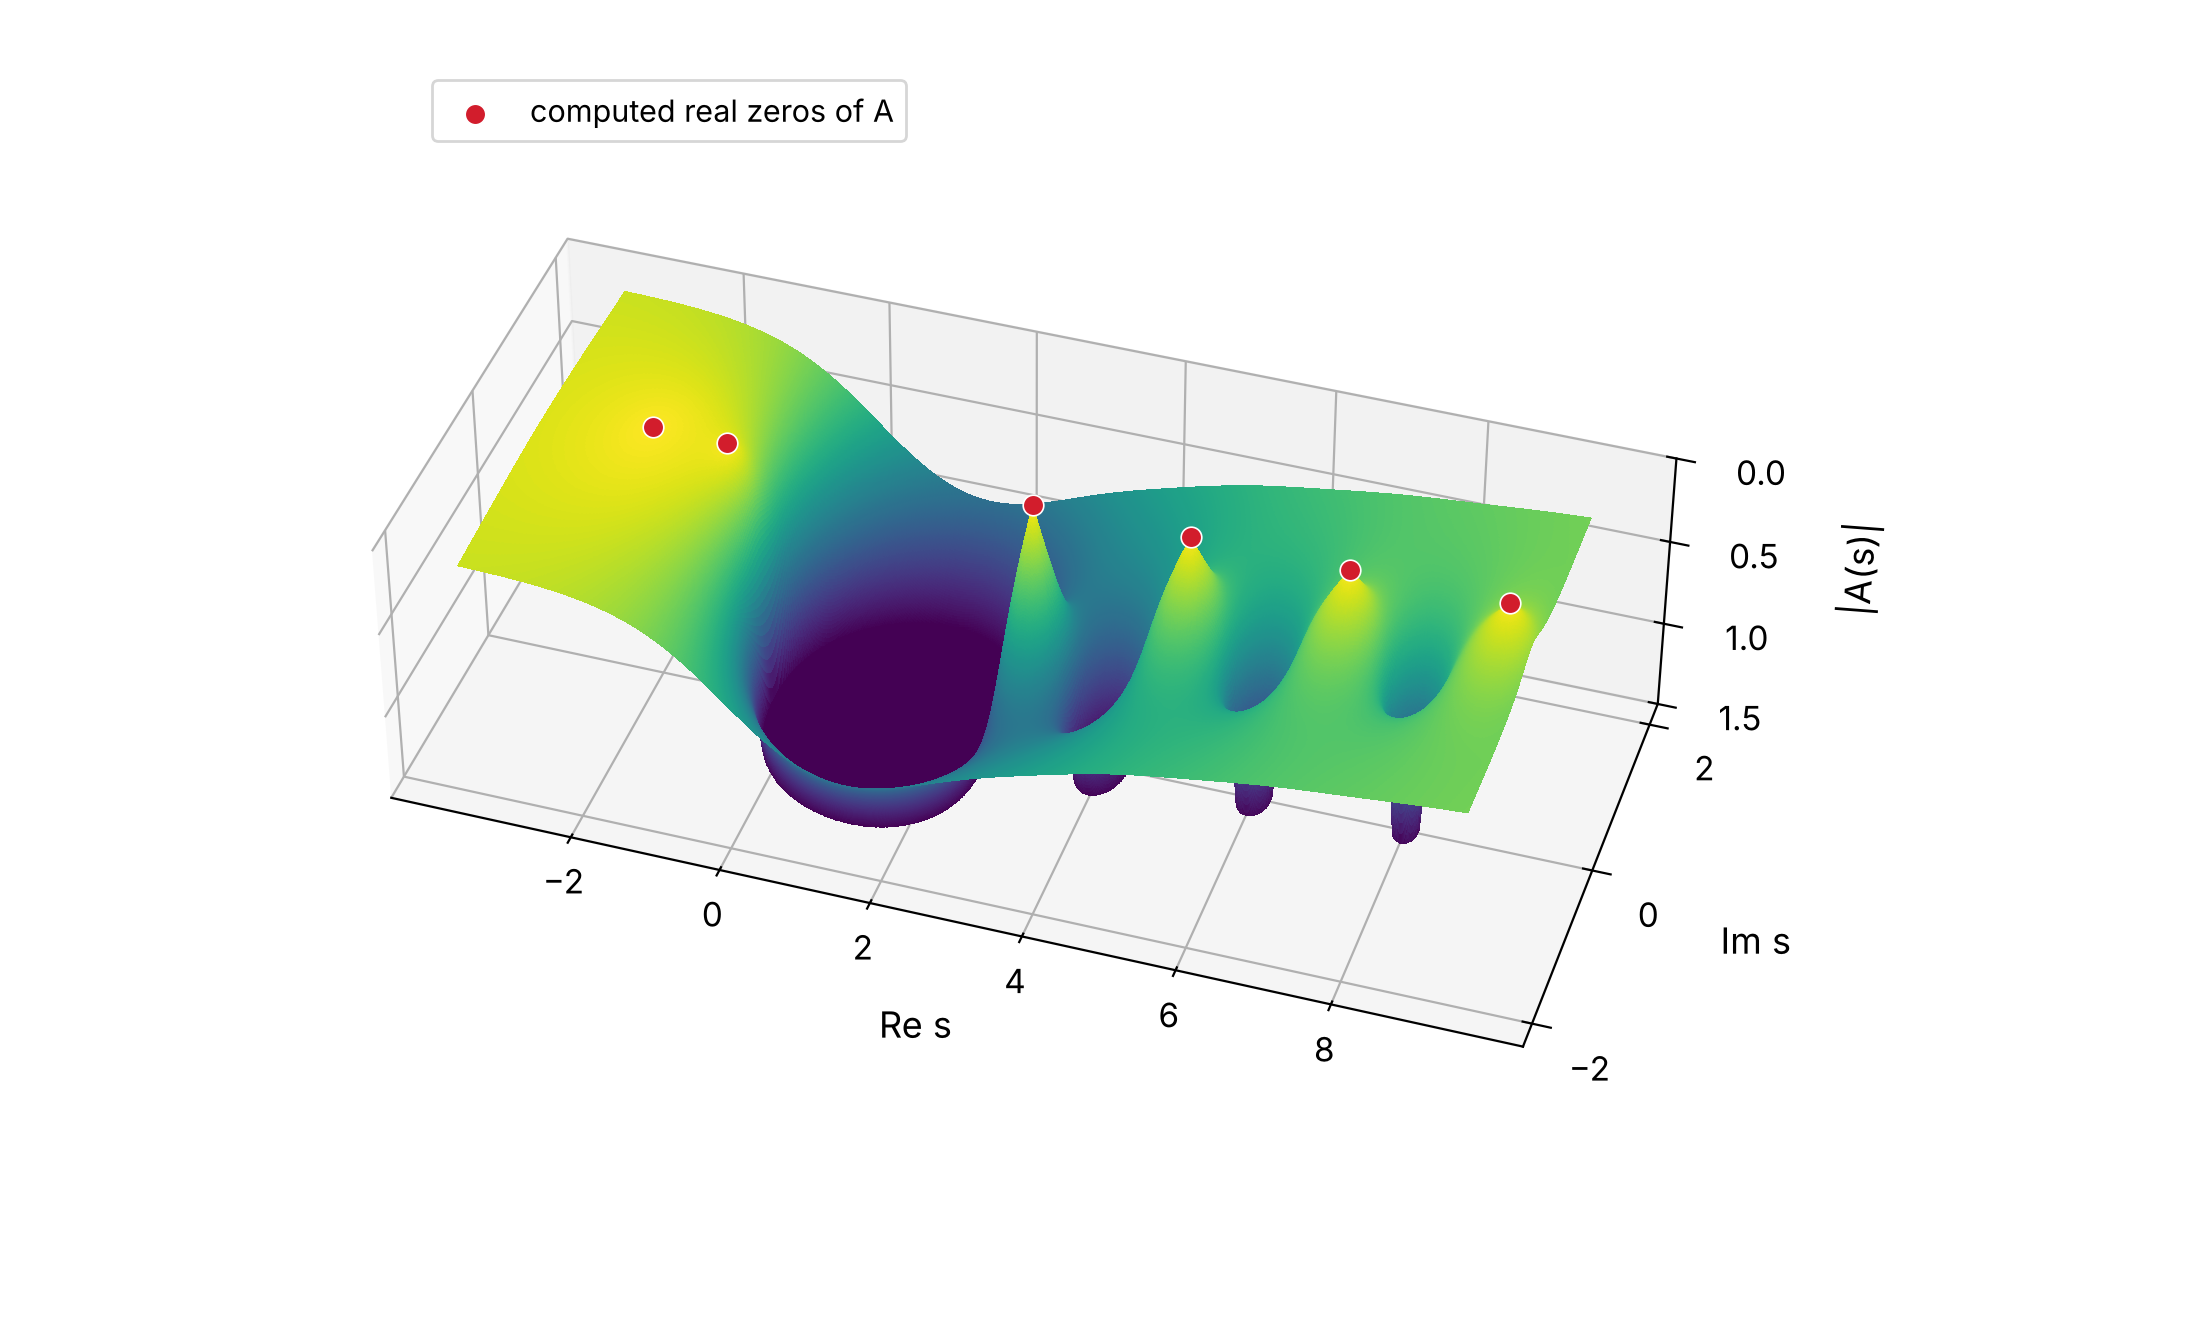
\includegraphics[width=.88\textwidth]{fig_A_real_surface.png}
\caption{$|A(s)|$ near the real axis, computed from \CGeqref{eq:Aseries} and clipped above $1.5$, with the vertical axis inverted. The red markers are the computed real zeros of $A$ of Table~\CGref{tab:zeros}; the wells are the poles $0,2,4,6,8$.}\label{fig:Areal}
\end{figure}

\begin{figure}[!htb]
\centering
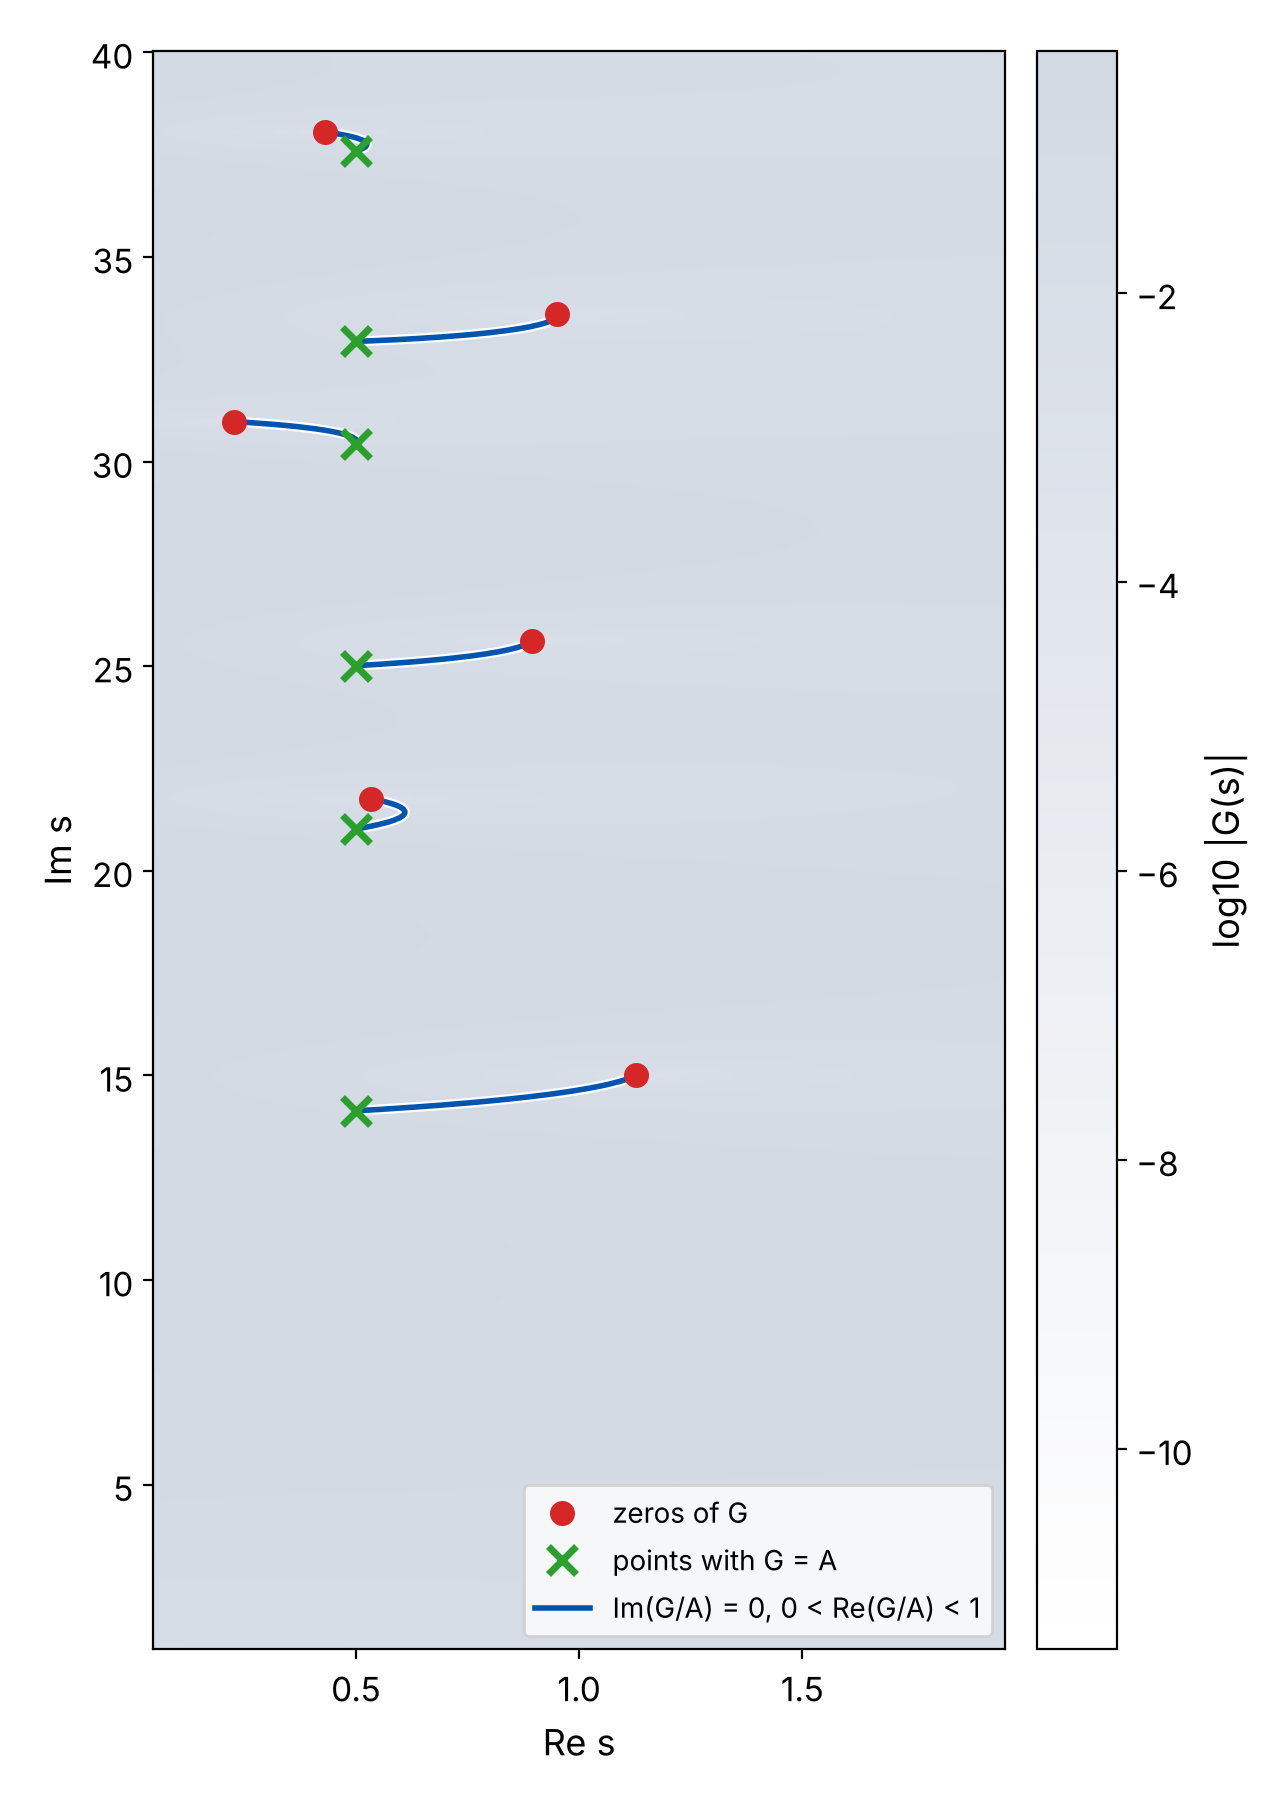
\includegraphics[width=.5\textwidth]{fig_zero_map.png}
\caption{Computed zeros of $G$ (dots), points with $G=A$ (crosses), and arcs of $\operatorname{Im}(G/A)=0$ with $0<\operatorname{Re}(G/A)<1$. Each arc joins a zero of $G$ to a point with $G=A$; this pairing is an observation on the computed data.}\label{fig:map}
\end{figure}

\clearpage
\section{Conclusions}\label{sec:concl}

The main conclusion is the bound \CGeqref{eq:boundCg}. For a two-level probe coupled dispersively to a thermal mode, the geometric mean of the Ramsey contrast after the first return, taken with the weight $u^{-2}$, satisfies $p_0<\mathcal V_1<\frac12\exp(C_g)\,p_0$ for every positive occupation, where $p_0$ is the probability that the mode is empty and $C_g=0.743794\ldots$ is the log-sine constant \CGeqref{eq:Cg}. The two constants $1$ and $\frac12\exp(C_g)=1.05195\ldots$ cannot be improved. The log-sine constant is thus the sharp constant of a functional of the ideal contrast that can in principle be estimated from a sequence of Ramsey measurements: no thermal state gives a ratio $\mathcal V_1/p_0$ above $\frac12\exp(C_g)$, and every smaller constant is exceeded at a sufficiently high occupation.

The second conclusion states what this functional measures that the half-period contrast does not. For every photon statistics of compound Poisson type, including thermal, Poisson and displaced thermal statistics, $p_0<\mathcal V_1\le p_0^{\,1-c_1(1)}$ with $c_1(1)=0.0409\ldots$, so that the geometric contrast determines $\log p_0$ within $4.1$ per cent without a hypothesis on the statistics; the half-period contrast is the modulus of the mean parity and, for a given $p_0$, can take any value between $p_0^2$ and $1$ (Proposition~\CGref{prop:cp}). Within the thermal model the half-period contrast gives $\bar n$ exactly and more simply.

The third conclusion concerns damping. In the rate equations of the damped mode the coherence differs from the ideal one by at most $4\bar n(\bar n+1)\kappa t$ (Proposition~\CGref{prop:damp}). For the geometric contrast over $1\le u\le U$ this requires $\kappa/\chi$ well below $1/\big(4\pi\bar n(\bar n+1)(2\bar n+1)U\big)$, a condition met at low occupation in long-lived modes and not at high occupation, and the half-period contrast is less affected (Corollary~\CGref{cor:damp}). The returns of the contrast measure the intrinsic decay of the probe and test the linearity of the shift.

Further conclusions follow from the same analysis. The bound holds for every power weight $u^{-s-1}$ with $s>0$, with the sharp constant $e^{-sG(s)}$, so that the function $G$ on the positive real axis is the logarithm of the sharp constant divided by $-s$ (Theorem~\CGref{thm:main}). For thermal states the occupation is bracketed by the geometric contrast alone, $1/\mathcal V_1-1<\bar n<\exp(C_g)/(2\mathcal V_1)-1$ (Corollary~\CGref{cor:bracket}), and the geometric and half-period contrasts satisfy the relation \CGeqref{eq:half}, which contains no parameter and which coherent states of mean photon number at least $0.3$ violate (Corollary~\CGref{cor:half}). At high occupation $\mathcal V_1=\frac12\exp(C_g)p_0\,q^{\pi^2/12-3/4}e^{R}$ with $0<R\le\frac{\tau^2}{\pi^2}(\frac52+\frac12\log\frac1\tau)$ (Theorem~\CGref{thm:hot}). A finite range of delays $1\le u\le U$ changes $\log\mathcal V_s$ by at most $U^{-s}\log(2\bar n+1)$ (Proposition~\CGref{prop:trunc}). The integral of the logarithm of the contrast over all delays with the weight $u^{-2}$ is exactly $-\pi^2\bar n$, and the first return separates it into a part within $C_g-\log2$ of $\log p_0$ and a part that carries the linear term (Proposition~\CGref{prop:sum}). The product $\mathcal P(N)$ of the contrasts at the harmonic delays $N/k$ satisfies $\mathcal P(N)^{1/N}\to\mathcal V_1$, with the explicit bound \CGeqref{eq:harm} for its logarithmic rate (Proposition~\CGref{prop:harm}).

At complex exponents $G$ is the hot limit of the transform of $\log(V/p_0)$ after the first return, and its zeros are the weights on which that excess has no component (Proposition~\CGref{prop:complex}). Together with the transform $A$ of the delays before the first return it satisfies $G-A=\frac\pi s\cot(\frac{\pi s}2)\zeta$, so that in the strip $0<\operatorname{Re}s<2$ the two transforms coincide at a non-real exponent exactly at the zeros of the Riemann zeta function (Proposition~\CGref{prop:A}). This is a consequence of an explicit factorisation and gives no information on the location of those zeros.

\begin{thebibliography}{99}

\bibitem{Blais2021}
A.~Blais, A.~L.~Grimsmo, S.~M.~Girvin and A.~Wallraff, Circuit quantum electrodynamics, \emph{Rev. Mod. Phys.} \textbf{93} (2021), 025005.
\href{https://doi.org/10.1103/RevModPhys.93.025005}{doi:10.1103/RevModPhys.93.025005};
\href{https://arxiv.org/abs/2005.12667}{arXiv:2005.12667}.

\bibitem{BorweinStraub2012}
J.~M.~Borwein and A.~Straub, Log-sine evaluations of Mahler measures, \emph{J. Aust. Math. Soc.} \textbf{92} (2012), 15--36.
\href{https://doi.org/10.1017/S1446788712000067}{doi:10.1017/S1446788712000067};
\href{https://arxiv.org/abs/1103.3893}{arXiv:1103.3893}.

\bibitem{Brune1990}
M.~Brune, S.~Haroche, V.~Lefevre, J.~M.~Raimond and N.~Zagury, Quantum nondemolition measurement of small photon numbers by Rydberg-atom phase-sensitive detection, \emph{Phys. Rev. Lett.} \textbf{65} (1990), 976--979.
\href{https://doi.org/10.1103/PhysRevLett.65.976}{doi:10.1103/PhysRevLett.65.976}.

\bibitem{ClerkUtami2007}
A.~A.~Clerk and D.~W.~Utami, Using a qubit to measure photon-number statistics of a driven thermal oscillator, \emph{Phys. Rev. A} \textbf{75} (2007), 042302.
\href{https://doi.org/10.1103/PhysRevA.75.042302}{doi:10.1103/PhysRevA.75.042302};
\href{https://arxiv.org/abs/cond-mat/0611759}{arXiv:cond-mat/0611759}.

\bibitem{DLMF}
\emph{NIST Digital Library of Mathematical Functions}, edited by F.~W.~J.~Olver, A.~B.~Olde Daalhuis, D.~W.~Lozier, B.~I.~Schneider, R.~F.~Boisvert, C.~W.~Clark, B.~R.~Miller, B.~V.~Saunders, H.~S.~Cohl and M.~A.~McClain,
\href{https://dlmf.nist.gov/}{https://dlmf.nist.gov/}, consulted on 12 November 2026. No DOI.

\bibitem{DykmanKrivoglaz1987}
M.~I.~Dykman and M.~A.~Krivoglaz, Zero-phonon lineshape of impurity centers interacting with local or quasilocal vibrations, \emph{Fiz. Tverd. Tela} \textbf{29} (1987), 368--376; English translation in \emph{Sov. Phys. Solid State} \textbf{29} (1987), 210. No DOI;
\href{https://www.mathnet.ru/eng/ftt900}{https://www.mathnet.ru/eng/ftt900}.

\bibitem{Glauber1963}
R.~J.~Glauber, Coherent and incoherent states of the radiation field, \emph{Phys. Rev.} \textbf{131} (1963), 2766--2788.
\href{https://doi.org/10.1103/PhysRev.131.2766}{doi:10.1103/PhysRev.131.2766}.

\bibitem{Gambetta2006}
J.~Gambetta, A.~Blais, D.~I.~Schuster, A.~Wallraff, L.~Frunzio, J.~Majer, M.~H.~Devoret, S.~M.~Girvin and R.~J.~Schoelkopf, Qubit-photon interactions in a cavity: measurement-induced dephasing and number splitting, \emph{Phys. Rev. A} \textbf{74} (2006), 042318.
\href{https://doi.org/10.1103/PhysRevA.74.042318}{doi:10.1103/PhysRevA.74.042318};
\href{https://arxiv.org/abs/cond-mat/0602322}{arXiv:cond-mat/0602322}.

\bibitem{Johnson2010}
B.~R.~Johnson, M.~D.~Reed, A.~A.~Houck, D.~I.~Schuster, L.~S.~Bishop, E.~Ginossar, J.~M.~Gambetta, L.~DiCarlo, L.~Frunzio, S.~M.~Girvin and R.~J.~Schoelkopf, Quantum non-demolition detection of single microwave photons in a circuit, \emph{Nature Phys.} \textbf{6} (2010), 663--667.
\href{https://doi.org/10.1038/nphys1710}{doi:10.1038/nphys1710};
\href{https://arxiv.org/abs/1003.2734}{arXiv:1003.2734}.

\bibitem{Milul2023}
O.~Milul, B.~Guttel, U.~Goldblatt, S.~Hazanov, L.~M.~Joshi, D.~Chausovsky, N.~Kahn, E.~\c{C}ifty\"urek, F.~Lafont and S.~Rosenblum, Superconducting cavity qubit with tens of milliseconds single-photon coherence time, \emph{PRX Quantum} \textbf{4} (2023), 030336.
\href{https://doi.org/10.1103/PRXQuantum.4.030336}{doi:10.1103/PRXQuantum.4.030336};
\href{https://arxiv.org/abs/2302.06442}{arXiv:2302.06442}.

\bibitem{Peng2015}
X.~Peng, H.~Zhou, B.-B.~Wei, J.~Cui, J.~Du and R.-B.~Liu, Experimental observation of Lee--Yang zeros, \emph{Phys. Rev. Lett.} \textbf{114} (2015), 010601.
\href{https://doi.org/10.1103/PhysRevLett.114.010601}{doi:10.1103/PhysRevLett.114.010601};
\href{https://arxiv.org/abs/1403.5383}{arXiv:1403.5383}.

\bibitem{Rigetti2012}
C.~Rigetti, J.~M.~Gambetta, S.~Poletto, B.~L.~T.~Plourde, J.~M.~Chow, A.~D.~C\'orcoles, J.~A.~Smolin, S.~T.~Merkel, J.~R.~Rozen, G.~A.~Keefe, M.~B.~Rothwell, M.~B.~Ketchen and M.~Steffen, Superconducting qubit in a waveguide cavity with a coherence time approaching 0.1 ms, \emph{Phys. Rev. B} \textbf{86} (2012), 100506(R).
\href{https://doi.org/10.1103/PhysRevB.86.100506}{doi:10.1103/PhysRevB.86.100506};
\href{https://arxiv.org/abs/1202.5533}{arXiv:1202.5533}.

\bibitem{Schuster2007}
D.~I.~Schuster, A.~A.~Houck, J.~A.~Schreier, A.~Wallraff, J.~M.~Gambetta, A.~Blais, L.~Frunzio, J.~Majer, B.~Johnson, M.~H.~Devoret, S.~M.~Girvin and R.~J.~Schoelkopf, Resolving photon number states in a superconducting circuit, \emph{Nature} \textbf{445} (2007), 515--518.
\href{https://doi.org/10.1038/nature05461}{doi:10.1038/nature05461};
\href{https://arxiv.org/abs/cond-mat/0608693}{arXiv:cond-mat/0608693}.

\bibitem{Scigliuzzo2020}
M.~Scigliuzzo, A.~Bengtsson, J.-C.~Besse, A.~Wallraff, P.~Delsing and S.~Gasparinetti, Primary thermometry of propagating microwaves in the quantum regime, \emph{Phys. Rev. X} \textbf{10} (2020), 041054.
\href{https://doi.org/10.1103/PhysRevX.10.041054}{doi:10.1103/PhysRevX.10.041054};
\href{https://arxiv.org/abs/2003.13522}{arXiv:2003.13522}.

\bibitem{Sears2012}
A.~P.~Sears, A.~Petrenko, G.~Catelani, L.~Sun, H.~Paik, G.~Kirchmair, L.~Frunzio, L.~I.~Glazman, S.~M.~Girvin and R.~J.~Schoelkopf, Photon shot noise dephasing in the strong-dispersive limit of circuit QED, \emph{Phys. Rev. B} \textbf{86} (2012), 180504(R).
\href{https://doi.org/10.1103/PhysRevB.86.180504}{doi:10.1103/PhysRevB.86.180504};
\href{https://arxiv.org/abs/1206.1265}{arXiv:1206.1265}.

\bibitem{Sun2014}
L.~Sun, A.~Petrenko, Z.~Leghtas, B.~Vlastakis, G.~Kirchmair, K.~M.~Sliwa, A.~Narla, M.~Hatridge, S.~Shankar, J.~Blumoff, L.~Frunzio, M.~Mirrahimi, M.~H.~Devoret and R.~J.~Schoelkopf, Tracking photon jumps with repeated quantum non-demolition parity measurements, \emph{Nature} \textbf{511} (2014), 444--448.
\href{https://doi.org/10.1038/nature13436}{doi:10.1038/nature13436};
\href{https://arxiv.org/abs/1311.2534}{arXiv:1311.2534}.


\bibitem{WeiLiu2012}
B.-B.~Wei and R.-B.~Liu, Lee--Yang zeros and critical times in decoherence of a probe spin coupled to a bath, \emph{Phys. Rev. Lett.} \textbf{109} (2012), 185701.
\href{https://doi.org/10.1103/PhysRevLett.109.185701}{doi:10.1103/PhysRevLett.109.185701};
\href{https://arxiv.org/abs/1206.2077}{arXiv:1206.2077}.

\bibitem{Yan2018}
F.~Yan, D.~Campbell, P.~Krantz, M.~Kjaergaard, D.~Kim, J.~L.~Yoder, D.~Hover, A.~Sears, A.~J.~Kerman, T.~P.~Orlando, S.~Gustavsson and W.~D.~Oliver, Distinguishing coherent and thermal photon noise in a circuit quantum electrodynamical system, \emph{Phys. Rev. Lett.} \textbf{120} (2018), 260504.
\href{https://doi.org/10.1103/PhysRevLett.120.260504}{doi:10.1103/PhysRevLett.120.260504}.

\end{thebibliography}

\end{document}

# BEGIN CORRECTVCG  (CorrectVCG checker, ignored by LaTeX; extract with the sed line at the top)
#!/usr/bin/env python3
r"""CorrectVCG checker (version 10) for Doktor's manuscripts and for Theorems and Proofs (TP).

Every .tex delivered to him carries a copy of this script after \end{document} (LaTeX never reads it).
Extract it with:   sed -n '/^# BEGIN CORRECTVCG/,/^# END CORRECTVCG/p' FILE.tex > correctvcg_check.py
Read every rule first:   python3 correctvcg_check.py --rules
Main uses:
    python3 correctvcg_check.py --paper FILE.tex                      format + mathematical checks of a manuscript
    python3 correctvcg_check.py CHAPTER.tex --chapter N --previous OLD  TP chapter
    python3 correctvcg_check.py --paper NEW.tex --diff OLD.tex --allowed labels.txt   no unrequested change
    python3 correctvcg_check.py FILE.tex --mark OUT.tex               review marks \VCGreviewed{n}
    python3 correctvcg_check.py FILE.tex --mark OUT.tex --reviewer codex     Codex marks \VCGreviewedCodex{n}
    python3 correctvcg_check.py FILE.tex --mark OUT.tex --reviewer chatgpt   ChatGPT marks \VCGreviewedChatGPT{n}
    python3 correctvcg_check.py FILE.tex --mark OUT.tex --reviewer copilot   Copilot marks \VCGreviewedCopilot{n}
    python3 correctvcg_check.py FILE.tex --embed OUT.tex              put this checker into a .tex
Exit code 0 only if there are no ERROR lines.  WARN lines must be read and fixed or justified one by one.
"""
import re
import sys
import argparse
import os
from collections import Counter

RULES = r'''
CorrectVCG RULES (v5). Every correction Doktor (Victor Casana-Giner) has had to make, mathematical and formal.
They apply to ALL his papers, notes, reviews and to every chapter of the book Theorems and Proofs (TP), not to one paper.
Read all of them before touching any of his .tex files. The past cases behind each rule are listed (in Spanish) in the
project docs claude/CorrectVCG-errores-matematicos-v4.md, claude/CorrectVCG-formato-v2.md, claude/CorrectVCG-listado-correcciones-v1.md.
This block and the checker below travel inside every .tex after \end{document}. NEVER remove them automatically:
they are removed only when Doktor himself asks for it (final versions).

RULE ZERO. Every error in what I deliver is mine, wherever it came from (source, other author, other AI, one of his drafts).
"It came from the source" is never an excuse.

THE NINE PATTERNS I REPEAT (check each one, in writing, before delivering anything):
 1. Marking a point as corrected without looking at the final output.
 2. Not running through the boundary cases: 0, negative values, 1, the first value of every index, empty ranges, degenerate parameters, the sign when dividing.
 3. Leaving symbols undefined, without domain, used before being defined, with two meanings, or renamed in only part of the text.
 4. Writing "equivalent", "suffices", "necessary", "unconditional" without both directions or the quantitative form.
 5. Leaving hard steps as "the same argument", "applies verbatim", "similarly", "as in [ref]".
 6. Marking a statement as verified without redoing the computations.
 7. Ignoring corrections he already gave: before delivering, run through all the accumulated rules.
 8. Fixing only the first occurrence of an error (first paragraph or section) and not the others.
 9. Importing results and errors from his papers and drafts without re-proving them, or citing him in the bibliography.
 And the one that annoys him most: in a revision, changing things that were right and breaking them. Only what he asks, or a proven error, changes; everything else stays letter by letter (checker: --diff OLD --allowed labels.txt).

ONE COMPLETE REVIEW SHOULD SUFFICE. Every review is complete, as if it were the only one: every statement, the whole checklist
below on each, every occurrence of every error, checker with 0 ERROR. In practice there will be several; none relaxes anything.
Every reviewed statement carries the reviewer's own mark in the LaTeX (n = number of reviews of that statement by that reviewer;
checker --mark --reviewer R): Claude \VCGreviewed{n}, Codex \VCGreviewedCodex{n}, ChatGPT \VCGreviewedChatGPT{n},
Copilot \VCGreviewedCopilot{n}.
Each reviewer touches only its own marks; the marks, counters and preamble block of the other reviewers stay letter by letter
(checker --diff gives ERROR otherwise). Review marks are not text changes and are ignored by every content check and by the
unrequested-change check. The embedded checker is never replaced by an older version (--embed refuses), and never removed unless
Doktor asks.

A. WHAT IS ASKED, AND APPLYING A CORRECTION REPORT
 A1. Deliver exactly the object asked (a chapter of TP is a chapter of TP, not a new version of its source paper; "only that part" means nothing else). A new version of a paper or of TP only when he asks.
 A2. If object or scope is unclear, ask ONCE before generating. Never regenerate "just in case".
 A3. For every report: point -> cause (mathematics / generator / text) -> where it is fixed -> LITERAL QUOTE of the corrected text in the FINAL OUTPUT. A point without that quote is not corrected.
 A4. Every correction in all its occurrences: grep the error and its variants (same symbol, formula, phrase, copies in settings, tooltips, abstract, introduction, other sections, other chapters, the checker, the skill); count before, 0 after. A general correction becomes a global convention, and every place that depended on it is revisited.
 A5. Never mark corrections as applied in block; each one is checked in the output.
 A6. Regression: in every new version re-check ALL points of ALL previous rounds.
 A7. If a report flags some cases of a pattern, search the pattern everywhere: there are usually more.
 A8. Mathematical errors are serious, never "minor". Referees' style recommendations are not applied. References cite the version actually checked (arXiv stays arXiv).

B. MATHEMATICAL CHECKLIST (each statement and proof, in writing; verified only after redoing every equality and boundary case)
 B1. Domains: every parameter, variable and index has its domain (N, Z, R, >=1, coprime, prime...) declared before use, in the statement or its setting.
 B2. First value of every index: substitute it into every sum, product, recurrence and induction; denominators, arithmetic functions and logarithms must be defined there (arguments >=1, nothing divided by 0, log of positive numbers). Counting from 0 or from 1 changes counts by one.
 B3. Division by zero: no denominator that can vanish for an allowed value of a parameter; the excluded value is treated separately.
 B4. Sign when dividing or multiplying an inequality by an expression whose sign depends on a parameter: each sign case separately. Excluded terms and the O(1) boundary values stated exactly.
 B5. Exact versus asymptotic: every "=" is exact; asymptotic steps carry their +o()/+O(); every intermediate equality redone.
 B6. Numerator and denominator: 1/min = max of reciprocals and conversely; a ratio defined as a/b never reappears as b/a; min/max read literally.
 B7. Exponents: braces (x^{-1}, never x^-1); x^{1/2+eps} not x^{1/2}+eps; the exponent of the statement equals the one at the end of the proof; the line with the total exponent written.
 B8. Floors and ceilings, ranges of blocks and windows; constants with all their dependencies; no loose bound passed off as sharp.
 B9. Symbols: every symbol and named object (norms, operators, transforms and their normalisation, coefficients, hypotheses with names) defined, with domain, before its first use; every new term defined or removed; quantifiers explicit. A letter that occurs once, in a formula of a proof, and nowhere else in the result, its proof or its Setting is undefined (usually a leftover of a renaming: o(log K) after K was renamed Y).
 B10. Collisions: one symbol, one meaning in the whole text (a fixed parameter is never also a summation index; a letter is never two different constants).
 B11. Renaming: a renamed symbol is renamed everywhere; never mix epsilon/varepsilon, phi/varphi, rho/varrho, theta/vartheta for one object, nor the same named hypothesis with different parameter letters.
 B12. Scope: "equivalent", "iff", "necessary", "suffices", "unconditional", "the theorem holds": both directions, the exact quantitative form used, the exact parameter range proved; a property of a sum is not a property of each summand; write the precise conclusion, not "the theorem holds".
 B13. Logical status: conditional on a named conjecture / classical unconditional / unconditional only through an external reference (say if it is an unrefereed preprint) / conditional on named hypotheses; every result in the right class; say what depends on which reference. A title that says "unconditional" may not hide a dependence on a cited result (proved only in a reference, e.g. an unrefereed preprint): the title says "unconditional through Theorem N" or the result goes to the conditional class.
 B14. An example satisfying a numerical inequality does not satisfy the structural hypotheses (multiplicativity, independence, ...) of the theorem it is compared with.
 B15. Nothing delegated: no "the same argument", "applies verbatim", "similarly", "as in [ref]", "standard" without statement and page at a load-bearing step. Write the intermediate lemma with every substitution, factor, congruence, Fourier inversion, the check that the hypotheses still hold, and every combinatorial fact used.
 B16. His own work: never cited as bibliography (no bibitem or \cite of Casana-Giner, Casanya, LawCasanya, Rotkiv Aynasac); his name appears only as author of the document itself. Nothing rests on his papers, drafts or compendium: whatever is taken from them is re-proved from scratch (drafts may be wrong; a draft is no authority).
 B17. Literature checked in LIBRARY TOTAL (GitHub repository vcasana1/LIBRARY-TOTAL-28oct2026, always accessible: git clone --filter=blob:none --no-checkout, then check out only INDEX.md and the PDFs needed; never say it is not reachable) (statement, hypotheses, page) ONCE: recorded at once in the registry claude/<paper>-fuentes-verificadas.md and never reopened (checker --verified). After compiling, look at the bibliography pages as PNG (checker --bib-pdf): DOI or arXiv in each entry, "(Cited on p. ...)", no [?] or ??.
 B18. When a statement passed B1-B17 with nothing found, go through B1-B4 and B12 again: the errors that escaped were there.

C. FORMAT OF EVERY .tex (canonical preamble of excursion_area_section_v39, in memory topics/latex-pdf-config)
 C1. Every displayed equation numbered on the right with \label (equation/align/gather/multline); never \[ \], $$ or starred environments for mathematics; \numberwithin{equation}{section}; amsart with reqno.
 C2. Links: v39 configuration (colorlinks=false, boxes: internal red, citations blue, URL/DOI teal; never hidelinks). All references with \CGref/\CGeqref, never \ref/\eqref; each \label with its CGTip tooltip inline in the preamble (no separate tips file). TOC. Every section with \label.
 C3. Bibliography: manual thebibliography, AuthorYear keys, DOI in every entry unless none exists (arXiv when appropriate), back-references "(Cited on p./pp. ...)".
 C4. Author: \author{Rotkiv Ayn\"asac} (never "Rotkin Aynasac"), no affiliation, e-mail rotkivanyasac@gmail.com below; or Victor Casana-Giner. Both are valid.
 C5. Prose: no itemize/enumerate in a paper; more full stops than semicolons; long paragraphs split. No "Questions"/"Open problems" sections; no heuristics (prove it or leave it out); no paper history (versions, retractions, referees); no "Provenance" paragraphs; no non-standard tags ([N], [C], [LIT]); explicit AMS status.
 C6. Words and symbols: clock, ordinate(s), envelope forbidden (also in labels, keys, captions); mu only Moebius; pi the prime-counting function and pi_RvM his; tau^c_k; no symbol with two meanings.
 C7. Appendices: \clearpage before \appendix and before each appendix.
 C8. Figures: PNG (never PDF images), never lower resolution; zip with figures at the root, Python code and its output.
 C9. Compile with pdflatex several passes: 0 errors, 0 undefined references, 0 multiply defined; a missing package is installed, never removed; the preamble is never changed to compile.
 C10. His papers: change only what he asks (words, commas, format untouched); propose exact lines and wait for his order; work on a copy and deliver the diff. A new version only when he asks.
 C11. Deliveries: .tex + .txt (literal copy) + .pdf as loose files and a zip that compiles; new integer version number in every file name; LaTeX and code in English; code in Python with its .txt.

D. THE BOOK THEOREMS AND PROOFS (TP)
 D1. Single edition: no edition, date, version or "supplement" marks.
 D2. Hyperlinks to everything. Literature in blue with [Literature]; background chapter of literature theorems.
 D3. Every entry has SettingBlock or SettingAsIn with the paragraphs defining its symbols and the displays it references (every \ref, \eqref, \CGref, \CGeqref, \autoref, \cref variant); copies identical to the original; settings never truncated.
 D4. Equation references never resolved to the id of the entry containing them; no self references; equation numbers = real chapter number, no gaps, every quoted number displayed.
 D5. No generator placeholder ("PROOF NOT LOCATED..."); a cited result carries "cited result" status with its reference. No corrupted text; umlauts as TeX accents.
 D6. Permanent ids (bookbuild/id_registry.json): never changed or reused; new = max+1.
 D7. Release with bookbuild/release.sh: VERSION, README version table, AI_GUIDE (where the database is; automatic publication of every version); old atlas/INDEX/SQLite deleted; id_registry.json and reviews/ kept. Say which version and commit were published. "sube git" means everything pending. Process improvements (checker, rules, docs) always go to correctpool at once, with no order needed; papers and drafts are never put on GitHub without his order; TP is released when he asks for a new version.

E. HONESTY IN THE ANSWER
 E1. Classical results are called classical from the first sentence, with their author; never disguised as new.
 E2. Work inside his programme and his own theorems; literature from LIBRARY TOTAL, not the web.
 E3. Never "corrected" without having seen it in the output. Report in each answer: the table of A3, the number of changed blocks (--diff) and that all were authorised, the number of reviewed statements and their review number, and what is still pending.
 E4. Chat in Spanish, formulas in LaTeX display, no "Provenance" or meta paragraphs at the end.
'''

KINDS = r'(?:Teorema|Lema|Proposici\\?\'?[oó]n|Corolario|Conjetura|Observaci\\?\'?[oó]n|Definici\\?\'?[oó]n|Theorem|Lemma|Proposition|Corollary|Conjecture|Remark|Definition|Hypothesis|Example|Condition|Assumption|Step|Part|Claim)'
FORBIDDEN_WORDS = [r'\bclock', r'\bordinates?\b', r'\benvelope']
OWN_NAMES = [r'Casa(?:\\~n|ñ|n|ny)a', r'Ayn(?:\\"a|ä|a)sac', r'Rotkiv']
LEFTOVERS = [
    (r'PROOF NOT LOCATED', 'generator placeholder left in the book'),
    (r'applies verbatim|verbatim the same|carries over verbatim|the same expansion leads to', 'proof step delegated instead of written out'),
    (r'H\s{2,}lder|H\?lder|H\ufffdlder', 'corrupted Hölder'),
    (r'\ufffd', 'mojibake character U+FFFD'),
    (r'[äöüÄÖÜ]', 'raw umlaut: use TeX accents (\\"o) in TP sources'),
]
EDITION_MARKS = [r'\bSupplement\b', r'\bsupplement(?:ary)? (?:to|of) (?:the )?(?:book|edition)',
                 r'\b(?:new|previous|this|second|first) edition\b', r'\bin version v?\d', r'(?<![./\w])v\d+\b(?![.](?:tex|n\d))']


def _braced(depth):
    """Regex for text with balanced braces nested up to depth levels (titles may contain \\ref{...}, \\textnormal{[\\ResolvedLink{..}{..}]})."""
    p = r'[^{}]*'
    for _ in range(depth):
        p = r'(?:[^{}]|\{' + p + r'\})*'
    return p


BRACED = _braced(6)


def entries(text):
    """Split into (uid, title, body) blocks by \\ResultHeading."""
    parts = re.split(r'(?=\\ResultHeading\{)', text)
    out = []
    for p in parts:
        m = re.match(r'\\ResultHeading\{(U\d{5})\}\{(' + BRACED + r')\}', p)
        if m:
            out.append((m.group(1), m.group(2), p))
    return out


def setting_spans(text):
    """Character spans of the arguments of \\SettingBlock{...} (balanced braces)."""
    spans = []
    for m in re.finditer(r'\\SettingBlock\{', text):
        depth, i = 1, m.end()
        while i < len(text) and depth:
            c = text[i]
            if c == '\\':
                i += 2
                continue
            depth += (c == '{') - (c == '}')
            i += 1
        spans.append((m.end(), i))
    return spans


PROOF_MARK = r'\\ProofHeading|\\begin\{proof\}'


def tp_statement(b, sp):
    """Statement of a TP entry: after its Setting (or after its heading notes) and before its proof.
    The note "PROOF INCLUDED" sits in the heading, so it never marks where the proof starts."""
    if sp:
        st = b[sp[-1][1]:]
    else:
        m = re.search(r'\\SourceNote\{[^{}]*(?:\{[^{}]*\}[^{}]*)*\}', b)
        st = b[m.end():] if m else b
    return re.split(PROOF_MARK, st, maxsplit=1)[0]


def setting_context(uid, byid, seen=None):
    """Everything a TP entry may rely on: its own Setting and, through SettingAsIn, the whole chain of earlier entries."""
    seen = set() if seen is None else seen
    if uid in seen or uid not in byid:
        return ''
    seen.add(uid)
    b = byid[uid]
    out = ''.join(b[x:y] for x, y in setting_spans(b))
    for r in re.findall(r'\\SettingAsIn\{(?:result:)?(U\d{5})\}', b):
        out += byid.get(r, '') + setting_context(r, byid, seen)
    return out


def balance(s):
    """Return a list of problems with braces and environments in s."""
    probs = []
    s2 = re.sub(r'\\[{}]', '', s)
    s2 = re.sub(r'(?<!\\)%.*', '', s2)
    depth = 0
    for ch in s2:
        if ch == '{':
            depth += 1
        elif ch == '}':
            depth -= 1
            if depth < 0:
                probs.append('closing brace without opening brace')
                depth = 0
    if depth:
        probs.append('%d unclosed brace(s)' % depth)
    stack = []
    for m in re.finditer(r'\\(begin|end)\{([^}]+)\}', s2):
        if m.group(1) == 'begin':
            stack.append(m.group(2))
        elif not stack or stack[-1] != m.group(2):
            probs.append('\\end{%s} does not match %s' % (m.group(2), stack[-1] if stack else 'nothing'))
        else:
            stack.pop()
    if stack:
        probs.append('unclosed environment(s): ' + ', '.join(stack))
    return probs


def check_paper(text, errors, warns):
    """Format rules for Doktor's manuscripts (LatexRules + excursion_area_section_v39 configuration)."""
    body = text.split('\\begin{document}', 1)[-1]
    pre = text.split('\\begin{document}', 1)[0]
    ctx = lambda m, t=body: t[max(0, m.start() - 50):m.end() + 50].replace('\n', ' ')
    # Every display numbered on the right and labelled.
    for m in re.finditer(r'(?<!\\)\\\[|\$\$', body):
        errors.append('unnumbered display (\\[ or $$): every display must be a numbered, labelled environment: %s' % ctx(m))
    for m in re.finditer(r'\\begin\{(equation|align|gather|multline|eqnarray)\*\}', body):
        errors.append('starred (unnumbered) display %s*: %s' % (m.group(1), ctx(m)))
    for m in re.finditer(r'\\begin\{(equation|align|gather|multline)\}(.*?)\\end\{\1\}', body, re.S):
        if '\\label' not in m.group(2):
            warns.append('numbered display without \\label: %s' % ctx(m))
    if 'reqno' not in pre and 'amsart' in pre:
        warns.append('amsart without reqno: equation numbers must be on the right')
    if not re.search(r'\\numberwithin\{equation\}\{section\}', pre):
        warns.append('missing \\numberwithin{equation}{section}')
    # Links with border + hover previews + back-references.
    if re.search(r'hidelinks|colorlinks\s*=\s*true', pre):
        errors.append('hidelinks/colorlinks=true: use the v39 configuration (colorlinks=false, boxed links)')
    for need, why in [('pagebackref', 'back-references (Cited on p. ...)'), ('pdfcomment', 'hover tooltips'),
                      (r'\\CGref', '\\CGref/\\CGeqref macros'), ('pdfborder', 'boxed links'), (r'\\backrefalt', 'Cited on p./pp. format')]:
        if not re.search(need, pre):
            errors.append('preamble lacks %s (%s)' % (need.replace('\\\\', '\\'), why))
    for m in re.finditer(r'(?<![A-Za-z@])\\(eq)?ref\{', body):
        errors.append('raw \\%sref: use \\CG%sref (hover preview): %s' % (m.group(1) or '', m.group(1) or '', ctx(m)))
    tips = set(re.findall(r'\\csname CGTip@([^\\]+)\\endcsname', pre))
    for lb in re.findall(r'\\label\{([^}]+)\}', body):
        if lb not in tips:
            warns.append('label %s has no CGTip tooltip in the preamble' % lb)
    for m in re.finditer(r'\\(section|subsection)\*?\{[^}]*\}(?!\s*\\label)', body):
        warns.append('%s without \\label: %s' % (m.group(1), ctx(m)))
    if '\\tableofcontents' not in body:
        warns.append('no \\tableofcontents')
    # Author.
    au = re.search(r'\\author(?:\[[^\]]*\])?\{([^}]*)\}', text)
    rotkiv = au and re.search(r'Rotkiv Ayn(?:\\"a|\\"\{a\}|ä)sac', au.group(1))
    civil = au and re.search(r'Casa(?:\\~n|\\~\{n\}|ñ)a-Giner', au.group(1))
    if not (rotkiv or civil):
        errors.append('author must be Rotkiv Ayn\\"asac or V\\\'ictor Casa\\~na-Giner (found: %s)' % (au.group(1) if au else 'no \\author'))
    if rotkiv and 'rotkivanyasac@gmail.com' not in text:
        warns.append('author e-mail rotkivanyasac@gmail.com missing')
    # Bibliography: thebibliography, DOI or arXiv in every item.
    for m in re.finditer(r'\\bibitem(?:\[[^\]]*\])?\{([^}]*)\}(.*?)(?=\\bibitem|\\end\{thebibliography\})', body, re.S):
        if not re.search(r'doi|arxiv', m.group(2), re.I):
            warns.append('reference %s without DOI or arXiv link' % m.group(1))
    # Prose, not AI-style lists; no Questions/Open problems; no heuristics; no version history.
    for m in re.finditer(r'\\begin\{(itemize|enumerate|description)\}', body):
        errors.append('%s list in the paper body: write prose: %s' % (m.group(1), ctx(m)))
    for m in re.finditer(r'\\section\*?\{[^}]*(Question|Open problem|Open Problem|Problems)[^}]*\}', body):
        errors.append('section of questions/open problems: %s' % ctx(m))
    for m in re.finditer(r'\\begin\{heuristic\}|[Hh]euristic(?:ally)?\b', body):
        warns.append('heuristic material: either prove it or remove it: %s' % ctx(m))
    for m in re.finditer(r'previous version|earlier version|this version|in version|(?<![A-Za-z\\])v\d+\b|retract|withdrawn claim|\breferee', body, re.I):
        errors.append('version-history / referee mention inside the paper: %s' % ctx(m))
    for m in re.finditer(r'[Pp]rocedencia|[Pp]rovenance', body):
        errors.append('provenance paragraph: %s' % ctx(m))
    for m in re.finditer(r'Platt|3\s*\\cdot\s*10\^\{?12', body):
        warns.append('result depending on numerical zero verification (Platt / 3e12): %s' % ctx(m))
    # Appendices start on a new page.
    for m in re.finditer(r'\\appendix', body):
        if not re.search(r'\\clearpage\s*$', body[:m.start()]):
            errors.append('\\appendix not preceded by \\clearpage')
        tail = body[m.end():]
        for s in re.finditer(r'\\section\{', tail):
            if not re.search(r'\\clearpage\s*$', tail[:s.start()]):
                errors.append('appendix section without \\clearpage before it: %s' % tail[s.start():s.start() + 60].replace('\n', ' '))


STANDARD_OPS = {'Re', 'Im', 'mod', 'div', 'li', 'Li', 'd', 'e', 'i', 'tr', 'rank', 'supp', 'sgn', 'lcm', 'gcd', 'card', 'meas', 'dist', 'diam', 'ord', 'deg', 'id', 'T'}


def lambda_convention(text):
    """A global convention fixing the domain of the arithmetic functions (terms with argument <= 0 dropped) covers affine arguments."""
    return re.search(r'defined only for (?:positive )?(?:integers )?\$?[a-z]\s*(?:\\ge|\\geq)\s*1|every sum[^.]{0,60}restricted to arguments|terms? (?:with|whose) (?:an )?argument[^.]{0,60}(?:omitted|excluded|dropped)', text)


MATH_ENVS = r'(?:theorem|lemma|proposition|corollary|conjecture|definition|remark|hypothesis|example)'


def math_units(text, paper):
    """Units for the mathematical pass: TP entries, or statement+proof blocks of a manuscript."""
    if not paper:
        return [(u, t, b) for u, t, b in entries(text)]
    out = []
    for m in re.finditer(r'\\begin\{(' + MATH_ENVS + r')\}(.*?)\\end\{\1\}(\s*\\begin\{proof\}.*?\\end\{proof\})?', text, re.S):
        lab = re.search(r'\\label\{([^}]+)\}', m.group(2))
        out.append((lab.group(1) if lab else 'line %d' % (text[:m.start()].count('\n') + 1), m.group(1), m.group(0)))
    return out


def _math_spans(t):
    """Text of every inline or displayed formula of t."""
    t = re.sub(r'(?<!\\)%.*', '', t)
    out = re.findall(r'\$([^$]+)\$', t)
    out += re.findall(r'\\begin\{(?:equation|align|gather|multline)\*?\}(.*?)\\end\{(?:equation|align|gather|multline)\*?\}', t, re.S)
    return out


def check_orphan_letters(units, errors):
    # TP: the unit is the entry with its Setting chain (ERROR); papers: the result, its proof and the preceding text (WARN)
    """B9: a single letter that occurs in a formula of a proof and nowhere else in the unit (statement, Setting, proof)
    is undefined; usually it is a leftover of a renaming (e.g. o(log K) after K was renamed Y)."""
    for uid, setting, stmt, proof in units:
        if not proof:
            continue
        everything = setting + ' ' + stmt + ' ' + proof
        seen = set()
        for f in _math_spans(proof):
            # a symbol introduced by a reference in the same sentence ("By Lemma 8.4 ... over $(A_X,B_X]$") is defined there
            i = proof.find(f)
            sentence = re.split(r'\.\s', proof[max(0, i - 300):i])[-1] if i >= 0 else ''
            if re.search(r'\\(?:ref|CGref|CGeqref|eqref|cite)\{|\\ResolvedLink\{', sentence):
                continue
            g = re.sub(r'\\(?:label|tag|ref|eqref|CGref|CGeqref|cite|ResolvedLink|UniqueTarget)\s*(?:\[[^\]]*\])?\{[^{}]*\}(?:\{[^{}]*\})?', ' ', f)
            g = re.sub(r'\\(?:mathrm|text|operatorname|mathbb|mathbf|mathcal|mathscr|mathfrak|textnormal)\s*(?:\{[^{}]*\}|\w)', ' ', g)
            g = re.sub(r'(?<![A-Za-z\\])[Oo]\s*(?:_\s*(?:\{[^{}]*\}|\w))?\s*(?:\\[Bb]igg?[lr]?|\\left)?\s*[(\[]', ' (', g)
            for v in sorted(set(re.findall(r'(?<![\\A-Za-z])([A-Za-z])(?![A-Za-z])', g)) - set('deio')):
                n = len(re.findall(r'(?<![\\A-Za-z])%s(?![A-Za-z])' % v, ' '.join(_math_spans(everything))))
                if n == 1 and v not in seen:
                    seen.add(v)
                    errors.append('MATH %s: the letter %s occurs once, in a formula of the proof, and is defined nowhere in the unit (leftover of a renaming?): %s' % (uid, v, re.sub(r'\s+', ' ', f)[:90]))


QUALIFIED = r'through|relative to|via|assuming|given|(?<!un)conditional|modulo|on Theorem|on Conjecture|of the cited'


def check_unconditional_titles(text, paper, errors, warns):
    """B13: a result whose title says "unconditional" may not depend on a cited result (proved only in a reference,
    e.g. an unrefereed preprint) unless the title says so ("unconditional through Theorem 7.1")."""
    if not paper:
        ents = entries(text)
        cited = {u for u, t, b in ents if re.search(r'\\StateNote\{CITED RESULT', b)}
        items = [(u, t, set(re.findall(r'result:(U\d{5})', b)) & cited - {u}) for u, t, b in ents]
    else:
        body = text.split('\\begin{document}', 1)[-1]
        envs = list(re.finditer(r'\\begin\{(' + REVIEW_ENVS + r')\}(?:\[((?:[^\[\]]|\[[^\]]*\])*)\])?(.*?)\\end\{\1\}', body, re.S))
        lab = lambda m: (re.search(r'\\label\{([^}]+)\}', m.group(3)) or [None, None])[1]
        cited = {lab(m) for m in envs if lab(m) and not re.search(r'\\begin\{proof\}', body[m.end():m.end() + 300])
                 and (re.search(r'\\cite', m.group(2) or '') or re.search(r'unrefereed|preprint', m.group(3)))}
        items = []
        for m in envs:
            # the environment and its proof, up to the next environment
            pm = re.match(r'\s*\\begin\{proof\}.*?\\end\{proof\}', body[m.end():], re.S)
            seg = m.group(3) + (pm.group(0) if pm else '')
            refs = set(re.findall(r'\\CG(?:eq)?ref\{([^}]+)\}', seg)) & cited - {lab(m)}
            items.append((lab(m) or m.group(1), m.group(2) or '', refs))
    for u, title, refs in items:
        if not refs or not re.search(r'unconditional', title, re.I) or re.search(QUALIFIED, title, re.I):
            continue
        strong = re.search(r'(?:^|[:,(]\s*)unconditional\b|unconditional\)?\s*$', re.sub(r'\\\w+\{[^{}]*\}|[{}]', '', title), re.I)
        msg = 'MATH %s: the title says "unconditional" but the result uses the cited result(s) %s, proved only in a reference: say "through ..." in the title or move it to the conditional class' % (u, ', '.join(sorted(refs)))
        (errors if strong else warns).append(msg + ('' if strong else ' (check the wording)'))


def check_math(text, paper, warns, errors):
    """Patterns of the mathematical errors that Doktor had to correct (see RULES, section B).
    These are candidates: every MATH line is checked by hand against RULES section B."""
    defs = {}
    # a global convention fixing the domain of lambda/mu (and dropping terms with argument <= 0) covers affine arguments
    convention = lambda_convention(text)
    # a letter used as a parameter of a named hypothesis, e.g. LU_k(A,K), and also assigned a value elsewhere
    params = set(re.findall(r'\\mathrm\{[A-Z]+\}_\{?\w*\}?\(\s*([A-Z])\s*,', text))
    for v in sorted(params):
        for m in re.finditer(r'(?<![A-Za-z\\_{])%s\s*(?::=|=)\s*(e\^|\\exp|[0-9])' % v, text):
            warns.append('MATH symbol %s is a parameter of a named hypothesis and is also assigned a value: %s' % (v, text[max(0, m.start() - 60):m.end() + 30].replace('\n', ' ')))
            break
    for uid, kind, b in math_units(text, paper):
        flat = re.sub(r'\s+', ' ', b)
        c = lambda m: flat[max(0, m.start() - 60):m.end() + 40]
        # 3a. division by a parameter whose stated range contains 0
        for m in re.finditer(r'(?:/\(|/|\\frac\{[^{}]*\}\{)\s*([a-z]?)\s*([a-zA-Z])\s*(?:\)|\})', flat):
            v = m.group(2)
            if v in 'nkpqmdNXYTHxzw':
                continue
            near = flat[max(0, m.start() - 120):m.end() + 120]
            if re.search(r'\\mathbf\s*1_\{?%s\s*>\s*0|%s\s*>\s*0|%s\s*\\ne(?:q)?\s*0|%s\s*(?:\\ge|\\geq|>)\s*1' % (v, v, v, v), near):
                continue
            if re.search(r'(?<![A-Za-z\\_{])%s\s*(?:\\ge|\\geq|\\geqslant)\s*0|(?<![A-Za-z\\_{])%s\s*\\in\s*\\mathbb\s*\{?[RZ]' % (v, v), flat):
                warns.append('MATH %s: division by %s while %s=0 is allowed -- treat %s=0 separately: %s' % (uid, v, v, v, c(m)))
        # 3a. an arithmetic function at an affine argument with no positivity condition in the unit
        for m in re.finditer(r'\\(lambda|mu|Lambda|Omega|omega|tau|sigma|varphi)\(\s*([^()]*?[a-zA-Z]\s*[a-zA-Z]?\s*[+-]\s*[^()]*?)\)', flat):
            if not convention and not re.search(r'\\ge\s*1|\\geq\s*1|\\ge 1|>\s*0|\\geq 1|\\mathbb\s*\{?N|positive', flat):
                warns.append('MATH %s: \\%s(%s) at an affine argument, no condition making it >=1 in this unit' % (uid, m.group(1), m.group(2)[:30]))
                break
        # 3a. inequality divided by a factor whose sign depends on a parameter allowed to be negative
        negs = set(re.findall(r'(?<![A-Za-z\\_{])([a-zA-Z])\s*<\s*0|(?<![A-Za-z\\_{])([a-zA-Z])\s*\\in\s*\\mathbb\s*\{?[RZ]', flat))
        negs = {x or y for x, y in negs}
        if negs and re.search(r'[Dd]ivid|[Mm]ultipl\w* (?:both sides|the inequality|by)', flat):
            warns.append('MATH %s: an inequality is divided or multiplied while %s may be negative -- treat each sign separately' % (uid, ', '.join(sorted(negs))))
        # 3d. scope claims that need both directions / the quantitative form
        for m in re.finditer(r'equivalent to|if and only if|\\iff|\\Longleftrightarrow|necessary and sufficient|(?<!in)\bsufficient\b(?!ly)|it suffices|is necessary|is now (?:a theorem|unconditional|\\cite)|holds unconditionally|unconditionally', flat):
            warns.append('MATH %s: scope claim "%s" -- prove both directions, quantitative form, exact parameter range: %s' % (uid, m.group(0), c(m)))
        # 3e. unrefereed input used as unconditional
        if re.search(r'unconditional', flat) and re.search(r'\\cite', flat) and not re.search(r'preprint|unrefereed', flat):
            warns.append('MATH %s: "unconditional" next to a citation without saying whether it is a refereed result' % uid)
        # 3f. delegated steps
        for m in re.finditer(r'[Ss]imilarly|[Aa]nalogously|the same argument|the same expansion|the same proof|as in the proof of|as in the two-point case|mutatis mutandis|one checks|it is easy to see|easily seen|standard argument|by a standard|adaptation of|adapting|we omit|left to the reader|details are omitted', flat, re.I):   # also at the start of a sentence
            if re.match(r'[^.]{0,20}(?:written out|proved|carried out) in (?:Lemma|Proposition|Theorem|\\S|Section|\\CGref|~)', flat[m.end():m.end() + 60]):
                continue
            warns.append('MATH %s: delegated step "%s" -- write the step out: %s' % (uid, m.group(0), c(m)))
        # 3c. symbol given two different definitions
        for m in re.finditer(r'(?<![A-Za-z\\_^{])([A-Z])\s*(?::=|=)\s*(e\^\{[^}]*\}|\\[a-z]+\{?[^,;$]{0,15}|[0-9][^,;$]{0,10})', flat):
            defs.setdefault(m.group(1), {}).setdefault(re.sub(r'\s', '', m.group(2))[:20], uid)
    for v, d in defs.items():
        if len(d) > 1:
            warns.append('MATH symbol %s defined with %d different values (%s) -- one symbol, one meaning' % (v, len(d), '; '.join('%s in %s' % (k, u) for k, u in list(d.items())[:4])))
    # 3c. TP: \mathrm/\mathcal names in a statement that its Setting never defines
    if not paper:
        byid = {u: b for u, _, b in entries(text)}
        for uid, title, b in entries(text):
            sp = setting_spans(b)
            setting = setting_context(uid, byid)
            stmt = tp_statement(b, sp)
            for name in sorted(set(re.findall(r'\\mathrm\{([A-Z][A-Za-z]{1,4})\}', stmt))):
                if name not in setting and not re.search(r'(?:say|define|denote|let|write)[^.]{0,80}\\mathrm\{%s\}' % name, stmt, re.I):
                    warns.append('MATH %s: \\mathrm{%s} used in the statement but not defined in its Setting' % (uid, name))


# ---------------------------------------------------------------------------
# Deeper mathematical checks (first index values, reciprocals, domains,
# definitions before use) and bibliography (registry of verified sources,
# rendering of the bibliography pages of the PDF).

import random

def _to_py(expr):
    """Very small LaTeX -> Python arithmetic converter (no sympy needed)."""
    e = expr
    e = re.sub(r'\\left|\\right|\\,|\;|\\!|\\big|\\Big|\\bigl|\\bigr|\\Bigl|\\Bigr', '', e)
    e = re.sub(r'\\frac\s*\{([^{}]*)\}\s*\{([^{}]*)\}', r'((\1)/(\2))', e)
    e = re.sub(r'\\frac\s*(\w)\s*(\w)', r'((\1)/(\2))', e)
    e = re.sub(r'\\cdot|\\times', '*', e)
    e = re.sub(r'\\(log|exp|sqrt)\b', r'\1', e)
    e = e.replace('{', '(').replace('}', ')').replace('^', '**')
    e = re.sub(r'_\(?\w+\)?', '', e)                      # drop subscripts: a_1 -> a
    if re.search(r'\\[A-Za-z]', e):
        return None
    e = re.sub(r'(?<=[0-9A-Za-z)])\s*(?=[A-Za-z(])', '*', e)   # implicit products
    e = re.sub(r'\b(log|exp|sqrt)\*\(', r'\1(', e)
    return e


def _is_zero(expr, var, value):
    """True if expr vanishes identically (for random values of the other letters) when var=value."""
    py = _to_py(expr)
    if not py:
        return False
    import math
    vals = []
    for seed in (1, 2):
        rnd = random.Random(seed)
        env = {k: rnd.uniform(1.3, 3.7) for k in sorted(set(re.findall(r'[A-Za-z]', py))) if k not in ('log', 'exp', 'sqrt')}
        env.update(log=math.log, exp=math.exp, sqrt=math.sqrt)
        env[var] = value
        try:
            vals.append(eval(re.sub(r'\b%s\b' % var, '(%r)' % value, py), {'__builtins__': {}}, env))
        except ZeroDivisionError:
            return True
        except Exception:
            return False
    return all(abs(v) < 1e-12 for v in vals)


def _lower_limit(sub):
    """(variable, first value) of a summation/product subscript, if it can be read."""
    for pat, shift in [(r'^\s*([a-zA-Z])\s*=\s*(-?\d+)', 0), (r'(-?\d+)\s*\\le(?:q|qslant)?\s*([a-zA-Z])(?![A-Za-z])', 0),
                       (r'([a-zA-Z])\s*\\ge(?:q|qslant)?\s*(-?\d+)', 0), (r'(-?\d+)\s*<\s*([a-zA-Z])(?![A-Za-z])', 1),
                       (r'([a-zA-Z])\s*>\s*(-?\d+)', 1)]:
        m = re.search(pat, sub)
        if m:
            a, b = m.group(1), m.group(2)
            var, start = (b, int(a)) if a.lstrip('-').isdigit() else (a, int(b))
            return var, start + shift
    return None


def check_deep(text, paper, warns, errors):
    for uid, kind, b in math_units(text, paper):
        flat = re.sub(r'\s+', ' ', b)
        # First value of every summation/product index: denominators and arithmetic arguments.
        for m in re.finditer(r'\\(sum|prod)\s*_\s*\{((?:[^{}]|\{[^{}]*\})*)\}(\s*\^\s*(?:\{[^{}]*\}|\S))?', flat):
            sub = re.sub(r'\\substack\{|\\\\', ' ', m.group(2))
            ll = _lower_limit(sub)
            if not ll:
                continue
            var, start = ll
            summand = flat[m.end():m.end() + 160]
            summand = re.split(r'\\end\{|\\label|\\quad|\\qquad|\.\s|,\s+(?:where|and|so)|\\tag', summand)[0]
            dens = re.findall(r'\\frac\s*\{[^{}]*\}\s*\{([^{}]*)\}', summand) + re.findall(r'\\frac\s*\w\s*(\w)', summand) \
                + re.findall(r'/\s*\(([^()]*)\)', summand) + re.findall(r'/\s*([A-Za-z0-9_]+)', summand)
            for d in dens:
                if re.search(r'(?<![A-Za-z\\])%s(?![A-Za-z])' % var, d) and _is_zero(d, var, start):
                    errors.append('MATH %s: first value %s=%d makes the denominator %s zero in \\%s_{%s}' % (uid, var, start, d.strip(), m.group(1), m.group(2)[:40]))
            for f, arg in re.findall(r'\\(lambda|mu|Lambda|Omega|omega|tau|sigma|varphi|log)\s*\(([^()]*)\)', summand):
                if re.search(r'(?<![A-Za-z\\])%s(?![A-Za-z])' % var, arg):
                    py = _to_py(arg)
                    if py and not re.search(r'[A-Za-z]', re.sub(r'\b%s\b' % var, '', py)):
                        try:
                            val = eval(re.sub(r'\b%s\b' % var, '(%d)' % start, py), {'__builtins__': {}}, {})
                        except Exception:
                            continue
                        if (f != 'log' and val < 1) or (f == 'log' and val <= 0):
                            errors.append('MATH %s: first value %s=%d gives \\%s(%s) with argument %s' % (uid, var, start, f, arg.strip(), val))
                    elif f != 'log' and not lambda_convention(text):
                        warns.append('MATH %s: first value %s=%d in \\%s(%s): check the argument is >=1' % (uid, var, start, f, arg.strip()[:30]))
        # Numerator/denominator: reciprocal of a min/max, and a ratio defined one way and used the other.
        for m in re.finditer(r'\\(min|max)[^$]{0,60}?\\\}\s*\^\s*\{?-1|\\(min|max)[^$]{0,60}?\)\s*\^\s*\{?-1|(?:\\frac\s*\{?1\}?\s*\{|1/)\s*\\(min|max)', flat):
            warns.append('MATH %s: reciprocal of a min/max (1/min = max of reciprocals) -- check numerator and denominator: %s' % (uid, flat[max(0, m.start() - 40):m.end() + 40]))
    ratios = {}
    for m in re.finditer(r'(\\?[A-Za-z]+(?:_\{?\w+\}?)?)\s*:=\s*\\frac\s*\{([^{}]+)\}\s*\{([^{}]+)\}', text):
        ratios[m.group(1)] = (re.sub(r'\s', '', m.group(2)), re.sub(r'\s', '', m.group(3)))
    for name, (num, den) in ratios.items():
        for m in re.finditer(re.escape(name) + r'\s*=\s*\\frac\s*\{([^{}]+)\}\s*\{([^{}]+)\}', text):
            if (re.sub(r'\s', '', m.group(1)), re.sub(r'\s', '', m.group(2))) == (den, num):
                errors.append('MATH %s is defined as %s/%s but later written as %s/%s (numerator and denominator swapped)' % (name, num, den, den, num))

    # Domains declared and symbols defined before use.
    DOMAIN = r'(?:\\in|\\ge|\\geq|\\le|\\leq|>|<|\\ne|\\neq|:=|\\to|\\mid|\\subseteq|\\subset)'
    if not paper:
        byid = {u: b for u, _, b in entries(text)}
        for uid, title, b in entries(text):
            sp = setting_spans(b)
            ctxt = setting_context(uid, byid)
            stmt = tp_statement(b, sp)
            known = ctxt + stmt
            math = ' '.join(re.findall(r'\$([^$]+)\$', stmt))
            math = re.sub(r'\\(?:mathrm|text|operatorname|label|ref|tag|mathbb|mathbf|mathcal|mathscr|mathfrak)\s*(?:\{[^{}]*\}|\w)', ' ', math)
            math = re.sub(r'(?<![A-Za-z\\])[Oo]\s*(?:_\s*(?:\{[^{}]*\}|\w))?\s*\(', ' (', math)   # O(...), O_{p,q}(...)
            math = re.sub(r'U\^\s*(?:\{[^{}]*\}|\w)', ' ', math)                               # Gowers norms U^k
            bound = set(re.findall(r'\\(?:sum|prod|max|min|sup|inf|lim|int)\s*_\s*\{?\\?(?:substack\{)?\s*([a-zA-Z])', math))
            letters = set(re.findall(r'(?<![\\A-Za-z])([A-Za-z])(?![A-Za-z])', math)) - bound - set('edio')
            missing = []
            for v in sorted(letters):
                # a letter may be declared with a subscript (a_1,a_2\in\mathbb N, g_{\mathcal C}) and arguments (C_X(u):=)
                SUB = r'(?:\s*[_^]\s*(?:\{(?:[^{}]|\{[^{}]*\})*\}|\\?\w+|\*)){0,3}(?:\s*\([^()]*\))?'
                lst = r'(?<![A-Za-z\\])%s(?![A-Za-z])' % v + SUB + r'\s*(?:,\s*[A-Za-z]' + SUB + r'\s*)*'
                v_ = r'(?<![A-Za-z\\])%s(?![A-Za-z])' % v + SUB
                defined = (
                    # symbol set equal to something after write/put/let/set/define/denote/the value/there is, or at the start of a display line
                    # ($q=1$ after "when" or "if" is a condition, not a definition)
                    re.search(r'(?:\\q?quad|&|\\\\|\\begin\{[a-z*]+\}|(?:[Ww]rit(?:e|ing)|[Pp]ut|[Ll]et|[Ss]et|[Dd]efine|[Dd]enote|value|[Tt]here (?:is|are))\s+\$)\s*' + v_ + r'\s*=', known)
                    # inside a leading tuple set equal to a tuple: $(A_1,B_1,Q)=(1,0,1)$ (not $(p,q)=1$, a gcd condition)
                    or re.search(r'\$\s*\((?:[^()$]*[,(]\s*)?' + v_ + r'\s*[,)][^()$]*\)?\s*=\s*\(', known)
                    # let/define ... be, maps g:A\to B
                    or re.search(r'(?:[Ll]et|[Dd]efine|[Ww]rite|[Dd]enote)\s+\$\s*' + v_ + r'\s*(?::|\$\s*(?:be|denote|for))', known)
                    or re.search(v_ + r'\s*:\s*(?:\\mathbb|\\\{|[A-Z])', known)
                    # defined by reference: $G_y$ of Definition 9.3, the twists $b_i$ of [2]
                    or re.search(v_ + r'\s*\$\s*(?:of|as in|from|in)\s+(?:Definition|Lemma|Theorem|Proposition|Hypothesis|Subsection|Section|\\CG|\\ref|\\cite|\{?\\textnormal)', known)
                    or re.search(r'(?:sets?|intervals?|functions?|maps?|twists?|cutoffs?|coefficients?|sequences?|vectors?|famil(?:y|ies)|class(?:es)?|residues?|norms?)\s+\$\s*' + v_, known))
                if not defined and not re.search(lst + DOMAIN, known) and not re.search(r'(?:[A-Za-z]' + SUB + r'\s*,\s*)+%s' % v + SUB + r'\s*' + DOMAIN, known) \
                        and not re.search(r'(?:integers?|reals?|real numbers?|primes?|numbers?|parameters?|fixed|every|each|all|any|constants?)\s*\$?\s*(?:[A-Za-z](?:_\{?\w+\}?)?\s*,\s*)*%s(?![A-Za-z])' % v, known):
                    missing.append(v)
            if missing:
                warns.append('MATH %s: no domain/definition for %s in the statement or its Setting' % (uid, ', '.join(missing)))
    else:
        body = text.split('\\begin{document}', 1)[-1]
        names = set(re.findall(r'\\math(?:rm|cal|scr|frak)\s*\{([A-Za-z]{1,6})\}', body)) - STANDARD_OPS
        for nm in sorted(names):
            pat = r'\\math(?:rm|cal|scr|frak)\s*\{%s\}' % nm
            uses = [m.start() for m in re.finditer(pat, body)]
            dm = re.search(r'(?:[Dd]efine|[Dd]enote|[Ll]et|[Ww]rite|[Ss]ay that|[Cc]all)[^.]{0,120}' + pat + r'|' + pat + r'[^$.]{0,40}?(?::=|\\coloneqq)|\\begin\{(?:hypothesis|definition|conjecture)\}\[[^\]]*' + pat, body)
            if dm and uses and uses[0] < dm.start() - 200:
                warns.append('MATH \\mathrm{%s} is used (offset %d) before it is defined (offset %d): %s' % (nm, uses[0], dm.start(), body[uses[0]:uses[0] + 80].replace('\n', ' ')))
            if not dm and len(uses) > 1:
                warns.append('MATH \\mathrm{%s} is used %d times and never defined' % (nm, len(uses)))


def check_bib_registry(text, registry, warns):
    """References already verified in the original are listed in the registry (e.g. claude/<paper>-fuentes-verificadas.md);
    they are not re-checked.  The others must be checked once and added to the registry at once."""
    reg = open(registry, encoding='utf-8', errors='replace').read()
    keys = re.findall(r'\\bibitem(?:\[[^\]]*\])?\{([^}]*)\}', text)
    todo = [k for k in keys if k not in reg]
    print('BIB registry %s: %d of %d references already verified (do not re-check them)' % (registry, len(keys) - len(todo), len(keys)))
    for k in todo:
        warns.append('BIB %s not in the registry of verified sources: check it once in LIBRARY TOTAL and record it' % k)


def render_bib(pdf, outdir, errors, warns):
    """Render the bibliography pages of the compiled PDF as PNG (to be looked at) and check their text."""
    import subprocess, os
    os.makedirs(outdir, exist_ok=True)
    n = int(re.search(r'Pages:\s*(\d+)', subprocess.run(['pdfinfo', pdf], capture_output=True, text=True).stdout).group(1))
    full = subprocess.run(['pdftotext', '-layout', pdf, '-'], capture_output=True, text=True).stdout
    pages = full.split('\f')
    for m in re.finditer(r'\?\?|\[\?\]', full):
        errors.append('PDF: undefined reference or citation "%s": %s' % (m.group(0), full[max(0, m.start() - 60):m.end() + 20].replace('\n', ' ')))
    start = None
    for i in range(len(pages) - 1, -1, -1):
        if re.search(r'^\s*(References|Bibliography|REFERENCES|BIBLIOGRAPHY)\s*$', pages[i], re.M):
            start = i + 1
            break
    if not start:
        warns.append('PDF: no References/Bibliography page found')
        return
    subprocess.run(['pdftoppm', '-png', '-r', '110', '-f', str(start), '-l', str(n), pdf, os.path.join(outdir, 'bib')], check=True)
    bibtext = '\n'.join(pages[start - 1:])
    bibtext = bibtext.split(re.search(r'(References|Bibliography|REFERENCES|BIBLIOGRAPHY)', bibtext).group(0), 1)[-1]
    items = [x for x in re.split(r'\n\s*(?=\[\w[^\]]{0,30}\]\s)', bibtext) if x.strip()]
    for it in items:
        head = ' '.join(it.split())[:70]
        if not re.search(r'doi|arXiv|arxiv', it):
            warns.append('PDF bibliography: entry without DOI/arXiv as printed: %s' % head)
        if not re.search(r'Cited on', it):
            warns.append('PDF bibliography: entry without "(Cited on p. ...)": %s' % head)
    for f in sorted(os.listdir(outdir)):
        if f.startswith('bib') and f.endswith('.png'):
            print('BIB PNG to look at:', os.path.join(outdir, f))



def check_names_exponents(text, paper, warns, errors):
    """Variable collisions, renamings between parts of the text, and exponent errors."""
    body = text.split('\\begin{document}', 1)[-1] if paper else text
    # Renaming: variant letters for the same role used side by side.
    for a, b in [(r'\\epsilon\b', r'\\varepsilon\b'), (r'\\phi\b', r'\\varphi\b'), (r'\\rho\b', r'\\varrho\b'),
                 (r'\\theta\b', r'\\vartheta\b'), (r'\\kappa\b', r'\\varkappa\b')]:
        na, nb = len(re.findall(a, body)), len(re.findall(b, body))
        if na and nb:
            warns.append('MATH both %s (%d times) and %s (%d times) are used: same object renamed, or two objects too alike' % (a.strip('\\b').replace('\\\\', '\\'), na, b.strip('\\b').replace('\\\\', '\\'), nb))
    # Renaming: a named hypothesis or object written with different parameter letters in different places.
    sig = {}
    for m in re.finditer(r'\\mathrm\{([A-Z][A-Za-z]{0,5})\}\s*_\s*\{?([A-Za-z0-9\']{1,4})\}?\s*\(([^()]{1,30})\)', body):
        args = tuple(x.strip() for x in m.group(3).split(','))
        if all(re.fullmatch(r'\\?[A-Za-z]+', x) for x in args):
            sig.setdefault(m.group(1), {}).setdefault(args, body[:m.start()].count('\n') + 1)
    for nm, d in sig.items():
        if len(d) > 1:
            warns.append('MATH \\mathrm{%s} appears with different parameter letters: %s -- renamed in part of the text?' % (nm, '; '.join('(%s) line %d' % (', '.join(k), v) for k, v in d.items())))
    for uid, kind, b in math_units(text, paper):
        if not paper:      # in TP the Setting is context, not part of the statement or proof of the entry
            sp = setting_spans(b)
            b = ''.join(b[i] for i in range(len(b)) if not any(x <= i < y for x, y in sp)) if sp else b
        flat = re.sub(r'\s+', ' ', b)
        # Collision: a letter fixed as a parameter and also used as a summation/product index in the same unit.
        # "for every k" is a universal quantifier, not a fixed parameter: only Let / Fix / fixed fix a letter
        fixed = set(re.findall(r'(?:[Ll]et|[Ff]ix|fixed)\s*\$\s*([A-Za-z])\s*(?:\\ge|\\geq|\\in|>|,|\$)', flat))
        bound = set(re.findall(r'\\(?:sum|prod)\s*_\s*\{\s*(?:\\substack\{)?\s*(?:-?\d+\s*\\le(?:q)?\s*)?([A-Za-z])(?![A-Za-z])', flat))
        for v in sorted(fixed & bound):
            warns.append('MATH %s: %s is fixed as a parameter and also used as a summation index -- variable collision' % (uid, v))
        # Collision: one letter declared in two different sets in the same unit.
        doms = {}
        for m in re.finditer(r'(?<![A-Za-z\\_])([A-Za-z])\s*\\in\s*(\\mathbb\s*\{?[NZQRC]\}?)', flat):   # a subscript (q_i) is not the letter declared
            doms.setdefault(m.group(1), set()).add(re.sub(r'[\s{}]', '', m.group(2)))
        for v, d in doms.items():
            if len(d) > 1:
                warns.append('MATH %s: %s is declared in different sets (%s) in the same unit' % (uid, v, ', '.join(sorted(d))))
        # Exponents: braces, ambiguous 1/2+epsilon, statement vs end of proof.
        for m in re.finditer(r'\^\s*-\s*[0-9A-Za-z]', flat):
            errors.append('MATH %s: exponent without braces (renders only the sign): %s' % (uid, flat[max(0, m.start() - 20):m.end() + 10]))
        for m in re.finditer(r'\^\s*\{?\s*1/2\s*\}\s*\+\s*\\varepsilon|\^\s*\\frac12\s*\+\s*\\varepsilon|\^\s*\\tfrac12\s*\+\s*\\varepsilon', flat):
            errors.append('MATH %s: "+\\varepsilon" outside the exponent (x^{1/2}+eps instead of x^{1/2+eps}): %s' % (uid, flat[max(0, m.start() - 20):m.end() + 10]))
        for m in re.finditer(r'\}\s*\^\s*\{[^{}]*\}\s*\^\s*[{\w]', flat):
            warns.append('MATH %s: double superscript / nested exponent, check grouping: %s' % (uid, flat[max(0, m.start() - 20):m.end() + 10]))
        if re.search(PROOF_MARK, flat):
            stmt, proof = re.split(PROOF_MARK, flat, maxsplit=1)
            def exps(t):
                return set(re.sub(r'\s', '', x) for x in re.findall(r'(?:O\s*\(|\\ll|\\le|o\s*\()\s*[^$]{0,25}?(?<![A-Za-z])([XxNTBHY])\s*\^\s*\{([^{}]{1,25})\}', t) for x in [x[0] + '^' + x[1]])
            es, ep = exps(stmt), exps(proof[-1500:])
            for e in es:
                base = e.split('^')[0]
                ends = [x for x in ep if x.startswith(base + '^')]
                if ends and e not in ends:
                    warns.append('MATH %s: statement has %s but the end of the proof has %s -- check the exponent' % (uid, e, ', '.join(sorted(ends))))



# ---------------------------------------------------------------------------
# Unrequested changes, and review marks in LaTeX.

REVIEWERS = {
    # name: (macro, counter, colour name, rgb, label printed in the margin)
    'claude': ('VCGreviewed', 'VCGreviewcount', 'VCGgreen', '0,0.45,0.15', 'Claude'),
    'codex': ('VCGreviewedCodex', 'VCGreviewcountCodex', 'VCGblue', '0,0.25,0.7', 'Codex'),
    'chatgpt': ('VCGreviewedChatGPT', 'VCGreviewcountChatGPT', 'VCGorange', '0.75,0.35,0', 'ChatGPT'),
    'copilot': ('VCGreviewedCopilot', 'VCGreviewcountCopilot', 'VCGpurple', '0.45,0.1,0.55', 'Copilot'),
}


def review_preamble(reviewer='claude'):
    """Preamble block defining one reviewer's mark; each reviewer has its own macro, counter, colour and final total.
    The Claude block is exactly the one of checker v7, so files marked before stay recognised."""
    mac, cnt, col, rgb, who = REVIEWERS[reviewer]
    return (PREAMBLE_TEMPLATE.replace('@WHO@', who).replace('@MAC@', mac).replace('@CNT@', cnt)
            .replace('@COL@', col).replace('@RGB@', rgb))


PREAMBLE_TEMPLATE = r"""
% CorrectVCG review marks: every statement reviewed by @WHO@ carries \@MAC@{n},
% n = how many times that statement has been reviewed.  \VCGshowreviewsfalse hides the marks.
\makeatletter
\@ifundefined{@MAC@}{%
\newcounter{@CNT@}
\newif\ifVCGshowreviews \VCGshowreviewstrue
\definecolor{@COL@}{rgb}{@RGB@}
\newcommand{\@MAC@}[1]{\stepcounter{@CNT@}\ifVCGshowreviews\marginpar{\raggedright\tiny\textcolor{@COL@}{Reviewed by @WHO@\\ (review~#1)}}\fi}
\AtEndDocument{\ifVCGshowreviews\par\medskip\noindent{\small\textcolor{@COL@}{Statements reviewed by @WHO@: \arabic{@CNT@}.}}\fi}
}{}
\makeatother
"""


REVIEW_PREAMBLE = review_preamble('claude')
MARK_ANY = r'\\VCGreviewed(?:Codex|ChatGPT|Copilot)?\{\d+\}'


def mark_re(reviewer):
    return r'\\' + REVIEWERS[reviewer][0] + r'\{(\d+)\}'


def strip_review_marks(text):
    """Review marks and their preamble blocks are not text changes."""
    for r in REVIEWERS:
        text = text.replace(review_preamble(r) + '\n', '').replace(review_preamble(r), '')
    return re.sub(MARK_ANY, '', text)


def marks_by_unit(text, reviewer):
    """(unit, n) for every mark of one reviewer."""
    return sorted((unit_of(text, m.start()), int(m.group(1))) for m in re.finditer(mark_re(reviewer), text))

REVIEW_ENVS = r'(?:theorem|lemma|proposition|corollary|conjecture|definition|remark|hypothesis|example)'


def unit_of(text, pos):
    """Label of the statement (or TP entry) that contains position pos."""
    tp = [m for m in re.finditer(r'\\ResultHeading\{(U\d{5})\}', text[:pos])]
    if tp:
        return tp[-1].group(1)
    lab = [m for m in re.finditer(r'\\label\{([^}]+)\}', text[:pos])]
    return lab[-1].group(1) if lab else 'preamble'


def check_diff(old_path, text, allowed_path, errors, warns, reviewer='claude'):
    """Every change between the previous version and this one must be a requested correction.
    allowed_path lists, one per line, the labels / TP ids whose text may change."""
    import difflib
    old_text = strip_embedded(open(old_path, encoding='utf-8', errors='replace').read())
    for r in sorted(REVIEWERS):
        if r != reviewer and marks_by_unit(old_text, r) != marks_by_unit(text, r):
            errors.append('REVIEW marks of %s changed by %s: %s -> %s (only %s may touch them)' % (
                r, reviewer, marks_by_unit(old_text, r), marks_by_unit(text, r), r))
        if r != reviewer and (review_preamble(r) in old_text) != (review_preamble(r) in text):
            errors.append('REVIEW preamble block of %s added or removed by %s' % (r, reviewer))
    old = strip_review_marks(old_text).rstrip('\n').splitlines()
    text = strip_review_marks(text)
    new = text.rstrip('\n').splitlines()
    allowed = set()
    if allowed_path:
        allowed = {x.strip() for x in open(allowed_path, encoding='utf-8').read().split() if x.strip()}
    offsets, acc = [], 0
    for ln in new:
        offsets.append(acc)
        acc += len(ln) + 1
    n = 0
    for tag, i1, i2, j1, j2 in difflib.SequenceMatcher(None, old, new, autojunk=False).get_opcodes():
        if tag == 'equal':
            continue
        n += 1
        where = unit_of(text, offsets[min(j1, len(new) - 1)] if new else 0)
        snippet = (' '.join(old[i1:i2])[:90] + '  -->  ' + ' '.join(new[j1:j2])[:90]).replace('\t', ' ')
        if allowed and where not in allowed:
            errors.append('UNREQUESTED change in %s (lines %d-%d), not in the list of requested corrections: %s' % (where, j1 + 1, j2, snippet))
        elif not allowed:
            warns.append('CHANGE %d in %s (lines %d-%d): justify it with a requested correction or undo it: %s' % (n, where, j1 + 1, j2, snippet))
    print('DIFF against %s: %d changed blocks' % (old_path, n))


def mark_reviewed(path, out, which, reviewer='claude'):
    """Write a copy of path in which every reviewed statement carries the reviewer's mark (n incremented on each review).
    Only that reviewer's marks are added or incremented; every other reviewer's mark stays as it is."""
    mac = REVIEWERS[reviewer][0]
    full = open(path, encoding='utf-8').read()
    t = strip_embedded(full)
    tail = full[len(t):] if full.startswith(t) else ''
    if '\\newcommand{\\%s}' % mac not in t:
        t = t.replace('\\begin{document}', review_preamble(reviewer) + '\n\\begin{document}', 1)
    sel = None if which == 'all' else {x.strip() for x in open(which, encoding='utf-8').read().split() if x.strip()}
    count = [0]

    def bump(block, key):
        if sel is not None and key not in sel:
            return block
        count[0] += 1
        m = re.search(mark_re(reviewer), block)
        if m:
            return block[:m.start()] + '\\%s{%d}' % (mac, int(m.group(1)) + 1) + block[m.end():]
        return None

    def env(m):
        lab = re.search(r'\\label\{([^}]+)\}', m.group(0))
        key = lab.group(1) if lab else None
        b = bump(m.group(0), key)
        if b is not None:
            return b
        head = re.match(r'\\begin\{' + REVIEW_ENVS + r'\}(?:\[(?:[^\[\]]|\[[^\]]*\])*\])?(?:\s*\\label\{[^}]+\})?', m.group(0))
        rest = m.group(0)[head.end():]
        own = re.match(r'(?:' + MARK_ANY + r')*', rest).end()   # after the marks already there
        return m.group(0)[:head.end()] + rest[:own] + '\\%s{1}' % mac + rest[own:]
    if '\\ResultHeading{' in t:
        def entry(m):
            b = bump(m.group(0), m.group(1))
            if b is not None:
                return b
            i = m.start(2) - m.start(0) + len(m.group(2))
            own = re.match(r'(?:' + MARK_ANY + r')*', m.group(0)[i:]).end()
            return m.group(0)[:i + own] + '\\%s{1}' % mac + m.group(0)[i + own:]
        t = re.sub(r'\\ResultHeading\{(U\d{5})\}(\{' + BRACED + r'\})(?:(?!\\ResultHeading\{).)*', entry, t, flags=re.S)
    else:
        t = re.sub(r'\\begin\{(' + REVIEW_ENVS + r')\}.*?\\end\{\1\}', env, t, flags=re.S)
    head = EMBED_HEADER if full.startswith(EMBED_HEADER) else ''
    i = full.find('\n' + EMBED_BEGIN)
    open(out, 'w', encoding='utf-8').write(head + t + (full[i + 1:] if i >= 0 else ''))
    print('MARKED %d statements reviewed by %s in %s' % (count[0], REVIEWERS[reviewer][4], out))


def check_review_marks(text, paper, errors, reviewer='claude'):
    """After a review, every statement must carry this reviewer's mark."""
    own = '\\%s{' % REVIEWERS[reviewer][0]
    if '\\ResultHeading{' in text:
        for u, title, b in entries(text):
            if own not in b:
                errors.append('REVIEW mark of %s missing in %s (%s)' % (REVIEWERS[reviewer][4], u, title[:50]))
    else:
        for m in re.finditer(r'\\begin\{(' + REVIEW_ENVS + r')\}(.*?)\\end\{\1\}', text, re.S):
            if own not in m.group(2):
                lab = re.search(r'\\label\{([^}]+)\}', m.group(2))
                errors.append('REVIEW mark of %s missing in %s %s' % (REVIEWERS[reviewer][4], m.group(1), lab.group(1) if lab else 'line %d' % (text[:m.start()].count('\n') + 1)))


EMBED_BEGIN = '# BEGIN CORRECTVCG'
EMBED_END = '# END CORRECTVCG'
EMBED_HEADER = ('% CorrectVCG: after \\end{document} this file carries every correction rule and the checker (LaTeX ignores them).\n'
                '% Never remove that block unless Doktor asks. Before any change run:\n'
                "% sed -n '/^# BEGIN CORRECTVCG/,/^# END CORRECTVCG/p' THIS.tex > correctvcg_check.py && python3 correctvcg_check.py --rules && python3 correctvcg_check.py --paper THIS.tex\n")


def strip_embedded(text):
    """The checker never checks its own embedded copy (nor the header comment that announces it)."""
    i = text.find('\n' + EMBED_BEGIN)
    if i >= 0:
        text = text[:i + 1]
    return text.replace(EMBED_HEADER, '')


def embed(path, out):
    """Write a copy of path that carries this checker after \\end{document} and a header comment saying how to use it."""
    full = open(path, encoding='utf-8').read()
    i = full.find('\n' + EMBED_BEGIN)
    old = re.search(r'CorrectVCG checker \(version (\d+)\)', full[i:]) if i >= 0 else None
    mine = int(re.search(r'CorrectVCG checker \(version (\d+)\)', __doc__).group(1))
    if old and int(old.group(1)) > mine:
        raise SystemExit('%s already carries checker version %s, newer than this one (%d): extract and use that one' % (path, old.group(1), mine))
    t = strip_embedded(full)
    t = t.rstrip('\n') + '\n'
    if '\\end{document}' not in t:
        raise SystemExit('no \\end{document} in %s' % path)
    me = open(os.path.abspath(__file__), encoding='utf-8').read()
    # when run from a copy extracted with sed, drop its own BEGIN/END marker lines
    me = '\n'.join(l for l in me.splitlines() if not (l.startswith(EMBED_BEGIN) or l.startswith(EMBED_END))) + '\n'
    t = EMBED_HEADER + t + '\n' + EMBED_BEGIN + '  (CorrectVCG checker, ignored by LaTeX; extract with the sed line at the top)\n' + me.rstrip('\n') + '\n' + EMBED_END + '\n'
    open(out, 'w', encoding='utf-8').write(t)
    print('EMBEDDED checker (%d lines) in %s' % (me.count('\n') + 1, out))


def main():
    ap = argparse.ArgumentParser()
    ap.add_argument('file', nargs='?')
    ap.add_argument('--previous', help='previous version of the same chapter, to check that ids are stable')
    ap.add_argument('--verified', help='registry of verified sources (markdown); listed references are not re-checked')
    ap.add_argument('--bib-pdf', help='compiled PDF: render its bibliography pages as PNG and check them')
    ap.add_argument('--diff', help='previous version: every changed block must be a requested correction')
    ap.add_argument('--allowed', help='with --diff: labels / TP ids whose text may change (one per line)')
    ap.add_argument('--mark', help='write a copy with the review marks of --reviewer (Claude \\VCGreviewed{n}, Codex \\VCGreviewedCodex{n}, ChatGPT \\VCGreviewedChatGPT{n}, Copilot \\VCGreviewedCopilot{n}) to this path (then stop)')
    ap.add_argument('--mark-which', default='all', help='with --mark: "all" or a file of labels / TP ids reviewed')
    ap.add_argument('--require-review', action='store_true', help='ERROR for every statement without the review mark of --reviewer')
    ap.add_argument('--reviewer', default='claude', choices=sorted(REVIEWERS), help='who reviews: claude (default), codex, chatgpt or copilot; each has its own marks and never touches the others')
    ap.add_argument('--rules', action='store_true', help='print every correction Doktor has made (read before working)')
    ap.add_argument('--embed', help='write a copy of the .tex that carries this checker after \\end{document} (then stop)')
    ap.add_argument('--paper', action='store_true', help='check one of his manuscripts (format rules) instead of a TP chapter')
    ap.add_argument('--chapter', help='chapter number, e.g. 36 (inferred from tags if omitted)')
    a = ap.parse_args()
    if a.rules:
        print(RULES)
        return
    if a.embed:
        embed(a.file, a.embed)
        return
    if a.mark:
        mark_reviewed(a.file, a.mark, a.mark_which, a.reviewer)
        return
    marked = strip_embedded(open(a.file, encoding='utf-8', errors='replace').read())
    # review marks (of any reviewer) are invisible to every content check, so the result never depends on who reviewed
    text = re.sub(MARK_ANY, '', marked)
    errors, warns = [], []

    tags = re.findall(r'\\tag\{([^}]*)\}', text)
    ch = a.chapter or (Counter(t.split('.')[0] for t in tags).most_common(1)[0][0] if tags else None)
    targets = set(re.findall(r'\\UniqueTarget\{([^}]+)\}', text)) | set(re.findall(r'\\label\{([^}]+)\}', text)) \
        | set(re.findall(r'\\hypertarget\{([^}]+)\}', text)) | set(re.findall(r'\\NumberedFormula\{[^}]*\}\{([^}]+)\}', text))
    ids = [u for u, _, _ in entries(text)]
    idset = set(ids)

    # 1. Equation tags: no duplicates, no gaps inside this chapter.
    # Displays copied into Setting blocks repeat their tag; they must be identical to the original.
    settings = setting_spans(text)
    inside = lambda pos: any(a <= pos < b for a, b in settings)
    disp = {}
    for m in re.finditer(r'\\begin\{(equation\*?|align\*?|gather\*?|multline\*?)\}(.*?)\\end\{\1\}', text, re.S):
        for t in re.findall(r'\\tag\{([^}]*)\}', m.group(2)):
            body_eq = re.sub(r'\s+', '', m.group(2))
            disp.setdefault(t, []).append((inside(m.start()), body_eq))
    for t, lst in disp.items():
        originals = [b for ins, b in lst if not ins]
        if len(originals) > 1:
            errors.append('equation tag (%s) is displayed %d times outside Setting blocks' % (t, len(originals)))
        # A display that lives in source prose (not in an entry) appears in TP only inside Settings: allowed.
        ref = originals[0] if originals else lst[0][1]
        if any(b != ref for ins, b in lst if ins):
            errors.append('Setting copy of (%s) differs from the original display' % t)
    if ch and not a.paper:
        nums = sorted(int(t.split('.')[1]) for t in tags if re.fullmatch(r'%s\.\d+' % re.escape(ch), t))
        if nums:
            missing = sorted(set(range(nums[0], nums[-1] + 1)) - set(nums))
            if missing:
                errors.append('equation numbers missing in chapter %s: %s' % (ch, ', '.join('(%s.%d)' % (ch, k) for k in missing)))
        # every equation number quoted in the text must be displayed somewhere
        quoted = set(re.findall(r'\((%s\.\d+)\)' % re.escape(ch), re.sub(r'\\tag\{[^}]*\}', '', text)))
        for q in sorted(quoted - set(tags), key=lambda x: int(x.split('.')[1])):
            errors.append('(%s) is quoted but never displayed in the chapter' % q)

    # 2. Links must resolve.
    for lb in sorted(set(re.findall(r'\\ResolvedLink\{([^}]+)\}', text))):
        if lb not in targets:
            errors.append('ResolvedLink to missing target %s' % lb)
    for lb in sorted(set(re.findall(r'\\ref\{result:(U\d{5})\}', text))):
        if lb not in idset:
            warns.append('reference to entry %s outside this file (check it exists in the book)' % lb)
    for lb in sorted(set(re.findall(r'\\(?:CG)?(?:eq)?ref\{((?!result:)[^}]+)\}', text))):
        if lb not in targets:
            errors.append('raw \\ref/\\eqref/\\CGref to unknown label %s (generator did not resolve it)' % lb)

    # 3. Entry-level checks.
    for uid, title, body in entries(text):
        # an equation statement must not be replaced by the id of the theorem that contains it
        # The symptom: an entry id printed bare, without "Theorem~", "Lemma~", ... in front,
        # where the source referred to an equation inside that entry.
        for m in re.finditer(r'(\S{0,25}?)~?\\ref\{result:(U\d{5})\}', body):
            before = body[max(0, m.start() - 160):m.start() + len(m.group(1))]
            ok_single = re.search(KINDS + r's?(?:~|\s)*$', before)
            ok_list = re.search(KINDS + r's(?:~|\s)*(?:\\ref\{result:U\d{5}\}\s*(?:,|and|or|--)\s*)+(?:~|\s)*$', before)
            if not (ok_single or ok_list):
                errors.append('%s: bare entry id %s -- probably an equation reference resolved to the id of its theorem: %s'
                              % (uid, m.group(2), body[max(0, m.start() - 50):m.end() + 30].replace('\n', ' ')))
        sp = setting_spans(body)
        no_setting = ''.join(body[i] for i in range(len(body)) if not any(x <= i < y for x, y in sp)) if sp else body
        if re.search(r'\\ref\{result:%s\}' % uid, no_setting):
            errors.append('%s: entry refers to itself (circular reference)' % uid)
        for p in balance(re.sub(r'\\(?:begin|end)\{LitEntry\}', '', body)):
            errors.append('%s (%s): %s' % (uid, title[:50], p))
        sb = re.search(r'\\Setting(?:Block|AsIn)\{', body)
        if 'PROOF INCLUDED' in body and not sb and not title.lower().startswith(('remark', 'definition')):
            warns.append('%s (%s): no Setting block -- check that every symbol of the statement is defined' % (uid, title[:50]))

    # 4. Duplicate ids, id stability.
    for u, n in Counter(ids).items():
        if n > 1:
            errors.append('entry id %s used %d times' % (u, n))
    if a.previous:
        old = {t: u for u, t, _ in entries(strip_embedded(open(a.previous, encoding='utf-8', errors='replace').read()))}
        new = {t: u for u, t, _ in entries(text)}
        for t, u in new.items():
            if t in old and old[t] != u:
                errors.append('id changed for "%s": %s -> %s' % (t[:60], old[t], u))
        new_ids = set(new.values())
        for t in sorted(set(old) - set(new)):
            if old[t] not in new_ids:      # same id with a new heading (e.g. a number added) has not disappeared
                warns.append('entry disappeared since previous version: %s "%s"' % (old[t], t[:60]))

    # 5. Forbidden content.
    if a.paper:
        check_paper(text, errors, warns)
    else:
        # rule C1 holds for every .tex: a TP display is numbered (equation* with \tag) or it is an error
        for m in re.finditer(r'(?<!\\)\\\[|\$\$', text):
            where = unit_of(text, m.start())
            errors.append('unnumbered display (\\[ or $$) in %s: every display must be numbered: %s' % (where, text[m.start():m.start() + 70].replace('\n', ' ')))
    check_math(text, a.paper, warns, errors)
    check_unconditional_titles(text, a.paper, errors, warns)
    if not a.paper:
        byid = {u: b for u, _, b in entries(text)}
        units = []
        for u, _, b in entries(text):
            sp = setting_spans(b)
            parts = re.split(PROOF_MARK, b, maxsplit=1)
            units.append((u, setting_context(u, byid), tp_statement(b, sp), parts[1] if len(parts) > 1 else ''))
    else:
        body = text.split('\\begin{document}', 1)[-1]
        units = []
        for m in re.finditer(r'\\begin\{(' + REVIEW_ENVS + r')\}(.*?)\\end\{\1\}\s*(\\begin\{proof\}.*?\\end\{proof\})?', body, re.S):
            lab = re.search(r'\\label\{([^}]+)\}', m.group(2))
            units.append((lab.group(1) if lab else m.group(1), body[max(0, m.start() - 2500):m.start()], m.group(2), m.group(3) or ''))
    check_orphan_letters(units, errors if not a.paper else warns)
    check_deep(text, a.paper, warns, errors)
    check_names_exponents(text, a.paper, warns, errors)
    if a.diff:
        check_diff(a.diff, marked, a.allowed, errors, warns, a.reviewer)
    if a.require_review:
        check_review_marks(marked, a.paper, errors, a.reviewer)
    if a.verified:
        check_bib_registry(text, a.verified, warns)
    if a.bib_pdf:
        render_bib(a.bib_pdf, os.path.splitext(a.bib_pdf)[0] + '_bib_png', errors, warns)
    for pat in FORBIDDEN_WORDS:
        for m in re.finditer(pat, text, re.I):
            errors.append('forbidden word "%s" near: %s' % (m.group(0), text[max(0, m.start() - 40):m.end() + 40].replace('\n', ' ')))
    # His own work is never cited and never imported: his drafts may contain errors.  In a manuscript
    # his name is allowed only as author of the document itself, so only the bibliography and the citations are scanned.
    own_scope = text
    if a.paper:
        own_scope = '\n'.join(re.findall(r'\\begin\{thebibliography\}.*?\\end\{thebibliography\}', text, re.S)) \
            + '\n' + ' '.join(re.findall(r'\\cite[pt]?\*?(?:\[[^\]]*\])?\{([^}]*)\}', text))
    for pat in OWN_NAMES:
        for m in re.finditer(pat, own_scope):
            errors.append("his own work cited or imported (never cite Casana-Giner; his drafts may contain errors): %s"
                          % own_scope[max(0, m.start() - 60):m.end() + 40].replace('\n', ' '))
    body_txt = text.split('\\begin{document}', 1)[-1]
    for m in re.finditer(r'(?:our|my) (?:previous|earlier|forthcoming) (?:work|paper|note)|in preparation|forthcoming|\bdraft\b|compendium', body_txt, re.I):
        warns.append('material that may come from one of his drafts: re-prove it from scratch, a draft is no authority: %s'
                     % body_txt[max(0, m.start() - 60):m.end() + 40].replace('\n', ' '))
    for pat, why in LEFTOVERS:
        for m in re.finditer(pat, text):
            errors.append('%s: %s' % (why, text[max(0, m.start() - 40):m.end() + 40].replace('\n', ' ')))
    body_only = re.sub(r'\\SourceNote\{[^}]*\}', '', text)
    for pat in EDITION_MARKS:
        for m in re.finditer(pat, body_only):
            warns.append('possible edition/version mark: %s' % body_only[max(0, m.start() - 40):m.end() + 40].replace('\n', ' '))

    for e in errors:
        print('ERROR', e)
    for w in warns:
        print('WARN ', w)
    print('SUMMARY: %d entries, %d equation tags, %d errors, %d warnings' % (len(ids), len(tags), len(errors), len(warns)))
    sys.exit(1 if errors else 0)


if __name__ == '__main__':
    main()
# END CORRECTVCG
